
\documentclass[12pt,a4paper, xetex, hyperref]{book}

\usepackage{fontspec}
\setmainfont{Geneva} %% Geneva, Helvetica, Helvetica Neue
\usepackage{xunicode}
\usepackage{polyglossia}
\setmainlanguage{french}
\setotherlanguage{english}
\setotherlanguage[variant=ancient]{greek}
\setotherlanguage{latin}
\setotherlanguage{german}
\setotherlanguage{chinese}
\renewenvironment{latin}{\begin{hyphenrules}{latin}}%%
  {\end{hyphenrules}}


\usepackage{dtk-logos}
%% \usepackage{draftwatermark}
\usepackage{pdfpages} % pour inclure des docs pdf
%\usepackage{appendix}

\usepackage{fancybox}
%%%%%%%%%%%%%%%%%%%%%%%%%%%%%%%%%%%%%%%%%%%%%%%%%%%%%
% remove uppercase in headers
\usepackage{fancyhdr}
\renewcommand{\chaptermark}[1]{\markboth{#1}{}}
\renewcommand{\sectionmark}[1]{\markright{#1}}
\pagestyle{fancy}
\fancyhf{}
\fancyhead[LE,RO]{\thepage}
\fancyhead[LO]{\itshape\nouppercase{\rightmark}}
\fancyhead[RE]{\itshape\nouppercase{\leftmark}}
\renewcommand{\headrulewidth}{0pt}
%%%%%%%%%%%%%%%%%%%%%%%%%%%%%%%%%%%%%%%%%%%%%%%%%%%%%

\usepackage{xspace}

\usepackage{tikz}
\usepackage{tikzpagenodes}

% Paquets indispensables pour bclogo
\usepackage{graphicx}
\usepackage[tikz]{mdframed} % pour la coupure des boîtes
% \usepackage{xkeyval}
% \usepackage{ifthen}
% \usepackage{ifpdf}
% \usepackage{etoolbox}

% \usepackage[tikz]{bclogo}

\usepackage[%
            maxlevel=3,%
            autostyle=true,%
            french=guillemets*,%
            english=american,%
            autopunct=true%
            ]{csquotes}

\usepackage{quotchap}            
\usepackage{epigraph}
\usepackage{epipart}            

\usepackage{verbatim}

\usepackage{frcursive}
\usepackage{pifont}
\renewcommand{\footnoterule}{%%
\vspace*{0.2cm}%%
\ding{47}\hfill \centering Notes\hfill \ding{45}\vspace*{.2cm}\hrule\vspace*{.2cm}}

\usepackage{shorttoc}
\usepackage[french]{minitoc}

\usepackage{subfloat}

\usepackage{xcolor}

%%%%%%%%%%%%%%%%%%%%%%%%%%%%%%%%%%%%%%%%%%%%%%%%%%%%%%%%%%%%%%%%%%%%%%%%%%%
%%%% ENGLISH 
%%%%%%%%%%%%%%%%%
% Phrases en anglais
\newcommand{\exEN}[1]{%
  \textcolor{blue}{\textenglish{#1}}%
}

\newcommand{\uks}[1]{% uk sound
  \href{#1}{
\includegraphics[width=0.5cm, height=0.3cm]{../img/union-jack-mini}}%
}

\newcommand{\uss}[1]{% us sound
  \href{#1}{
\includegraphics[width=0.5cm, height=0.3cm]{../img/us-flag-mini}}%
}

\newcommand{\aus}[1]{% australian sound
  \href{#1}{
\includegraphics[width=0.5cm, height=0.3cm]{../img/aussie-flag-mini}}%
}

% Liens vers les bonnes prononciations phonétiques
\newcommand{\properukus}[2]{%
  \begin{center}
    (\uks{#1}\quad \uss{#2})
  \end{center}
}

% Liens pour les drapeaux cliquables à droite au dessus du titre
% de la section
% RCLF: Right Corner Linked Flags
% #1: sound 1, #2: link 1, #3: sound 2, #4: link 2
\newcommand{\RCLF}[4]{%
  \begin{tikzpicture}[remember picture,overlay]
    \node[anchor=east,inner sep=0pt] at (current page text
    area.east|-0,3cm) {#1$\Rightarrow$ \uks{#2}\quad #3$\Rightarrow$ \uss{#4}};
  \end{tikzpicture}
}


% Insertion des liens YouGlish
\newcommand{\youglish}[1]{%
\exEN{For more examples with the word ``#1'' click on the \href{https://youtu.be/sYmJLFEowaY}{flags} below:}%
  \begin{center}%
    (\uks{https://youglish.com/search/#1/uk}\quad\uss{https://youglish.com/search/#1/us}\quad\aus{https://youglish.com/search/#1/aus})%
  \end{center}%
}

% Liens vers mon blog www.doyouspeakenglish.fr
\newcommand{\dyse}[1]{%
  \footnote{Consultez mon
    article complet sur ce son en cliquant sur \url{http://doyouspeakenglish.fr/#1}}%
}

% Liens vers les sons de l'alphabet
% #1 : lettre, #2 : lien interne, #3 : phonétique
\newcommand{\letr}[3]{%
  \oxford{#1} \hyperlink{#2}{\wordref{#1}{#3}}
}


% Liens vers le livre How The Ell Brain Learns
\newcommand{\HTEBL}{%
    ~\href{https://amzn.to/2pSEAsm}{\exEN{How The Ell Brain Learns}}\xspace%
}

% Liens vers le livre a critical introduction to phonetics
\newcommand{\lodge}{%
  \href{https://amzn.to/2K45eHn}{\exEN{A Critical Introduction to Phonetics}}\xspace
}

% Liens vers le livre a manual of english phonetics and phonology
\newcommand{\bs}{%
  \href{https://amzn.to/2HV8BzG}{\exEN{A Manual of English Phonetics and
    Phonology}}\xspace %de \textsc{Paul Burleigh} et \textsc{Peter Skandera}
}

% Liens vers le livre Collins Practical Phonology and Phonetics
\newcommand{\cpp}{%
  \href{https://amzn.to/2HsmuUR}{\exEN{Pratical Phonetics and
      Phonology}}\xspace
  %de \textsc{Beverley S. Collins}
}

% Liens vers le livre Ogden Phonetics
\newcommand{\ogden}{%
  \href{https://amzn.to/2Kc0NKE}{\exEN{An Introduction to English Phonetics}}\xspace
  %de \textsc{Richard Ogden}
}

% Epigraphes maison
\newcommand\juxtaposed[2]%
  {\par\noindent
   \parbox[t]{3cm}{\raggedright#1}%
   \hfill
   \parbox[t]{2cm}{\raggedleft#2}%
   \bigskip\par
  }

%%%%%%%%%%%%%%%%%%%%%%%%%%%%%%%%%%%%%%%%%%%%%%%%%%%%%%%%%%%%%%%%%%%%%%%%%%%%
%%% FRANÇAIS
%%%%%%%%%%%%%%%%%%%%%%%%%%
% Traductions en français
\newcommand{\exFR}[1]{%
  \textcolor{orange}{\textcursive{#1}}%
}

% Liens vers le livre Français Lycée
\newcommand{\FL}{%
  ~\href{https://amzn.to/2vWXuUu}{\exFR{français lycée}}\xspace%
  %de Pierre Brunel\xspace%
}

% Liens vers le livre Grévisse de l'Enseignant
\newcommand{\GE}{%
  ~\href{https://amzn.to/2I0vT9J}{\exFR{Grévisse de l'enseignant}}\xspace%
}

% Liens vers le livre Honni soit qui mal y pense
\newcommand{\HSQMYP}{%
  ~\href{https://amzn.to/2Fp3KUq}{\exFR{Honni soit qui mal y pense}}%
}

% Liens vers le livre Anglais débutant
\newcommand{\ad}{%
  ~\href{https://amzn.to/2F5OhZa}{\exFR{Anglais débutant 1 leçon par
      jour pendant 3 mois}}\xspace%
}

% Liens vers le livre Bescherelle l'anglais pour tous
\newcommand{\besch}{%
  ~\href{https://amzn.to/2HiDBfI}{\exFR{Bescherelle l'anglais pour tous}}\xspace%
}


% \newcommand{\blocFR}[2]{%
%   \begin{bclogo}[couleur=blue!30, arrond=0.1, logo=\bcdfrance]{#1}
%     \exFR{#2}
%   \end{bclogo}
% }

%%%   BLOCS
\newmdenv[linecolor=red, frametitle=Exemple]{exemple}
\newmdenv[linecolor=red, frametitle=Citation]{citations}

% \newmdenv[%
%           linecolor=red,%
%           roundcorner=5pt,%
%           backgroundcolor=green!20,%
%           frametitle=Traduction,%
%           frametitlerule=true,%
%           frametitlebackgroundcolor=blue!20,%
%           ]{traduction}

\global\mdfdefinestyle{tradstyle}{%
  backgroundcolor=blue!20,%
  linecolor=red,%
  middlelinewidth=2pt,%
  frametitlerule=true,%
  apptotikzsetting={%
    \tikzset{mdfframetitlebackground/.append style={%
        shade,left color=blue!20, right color=blue}%
    }%
  },%
  frametitlerulecolor=green!60,%
  frametitlerulewidth=1pt,%
  innertopmargin=\topskip,%
}


\newcommand{\tradbloc}[4]{%
  {\flushleft
    \begin{mdframed}[%
      style=tradstyle,%
      frametitle={%
        \exFR{%
          \href{#1}{#2},%
          #3%
        }%
      }%
      ]
      \exFR{<<~#4~>>} 
    \end{mdframed}%
  }
}
              
\global\mdfdefinestyle{citestyle}{%
  backgroundcolor=orange!20,%
  linecolor=red,%
  middlelinewidth=2pt,%
  frametitlerule=true,%
  apptotikzsetting={%
    \tikzset{mdfframetitlebackground/.append style={%
        shade,left color=orange, right color=orange!20}%
    }%
  },%
  frametitlerulecolor=green!60,%
  frametitlerulewidth=1pt,%
  innertopmargin=\topskip,%
}

\newcommand{\citebloc}[4]{%
  {\flushleft
    \begin{mdframed}[%
      style=citestyle,%
      frametitle={%
        \exEN{%
          \href{#1}{#2},%
          #3%
        }%
      }%
      ]
      \exEN{``#4''} 
    \end{mdframed}%
  }
}

\mdfsetup{%
  middlelinecolor=red,%
  middlelinewidth=2pt,%
  backgroundcolor=green!20,%
  roundcorner=10pt%
}


% Longues citations : #1 largeur #2 source #3 punct 
% \newenvironment{\bigquote}[1]
%  {\begin{center}%
%     \shadowbox{%
%       \begin{minipage}{#1\textwidth}\end{minipage}}%
%  }%
%  {\end{center}}
    


%%%%%%%%%%%%%%%%%%%%%%%%%%%%%%%%%%%%%%%%%%%%%%%%%%%%%%%%%%%%%
% Phonétique
%%%%%%%%%%%%%%%%%%%%%%%%%%%%%%%%%%%%%%%%%%%%%%%%%%%%%%%%%%%%%
% Mots écrits en transcription phonétiques (donc PHONèMes)
\newcommand{\phonm}[1]{%
  \textcolor{teal}{/#1/}
}

% Liens vers wordreference
\newcommand{\wordref}[2]{%
  \href{http://www.wordreference.com/enfr/#1}{\phonm{#2}}
}

% Liens vers oxforddictionnaries
\newcommand{\oxford}[1]{%
  \href{https://en.oxforddictionaries.com/definition/#1}{\exEN{#1}}
}

% Liens vers cambridge
\newcommand{\cambridge}[1]{%
  \href{https://dictionary.cambridge.org/fr/dictionnaire/anglais/#1}%
  {\exEN{#1}}
}

% Exemple de mot avec Oxford
\newcommand{\exMotOx}[2]{%
  Le mot \exEN{\href{http://www.wordreference.com/enfr/#1}{#1}} qui
  s'écrit phonétiquement
  \href{https://en.oxforddictionaries.com/definition/#1}{\phonm{#2}}
}

% Exemple de mot avec Cambridge
\newcommand{\exMotCam}[2]{%
  Le mot \exEN{\href{http://www.wordreference.com/enfr/#1}{#1}} qui
  s'écrit phonétiquement
  \href{https://dictionary.cambridge.org/fr/dictionnaire/anglais/#1}{\phonm{#2}}
}

% Son isolé ou phone
\newcommand{\phon}[1]{%
  \textcolor{teal}{[#1]}
}

% Sons écrits en transcription phonétiques
\newcommand{\son}{%
  \textcolor{teal}{son}
}

% Notations
\newcommand{\notation}{%
  \begin{center}
    {\Large Attention aux \hyperlink{notation}{notations} !}
  \end{center}
}
% Présentation du nom du son avec les liens vers le blog et vers
% wikipédia
% \newcommand[7]{\sn}{% sound name
%   Ce \textcolor{red}{son} a pour nom technique\dyse{#1} :% #1: lien
%                                 % vers le blog
%   %
%   \begin{itemize}%
%   \item \exEN{#2\CW{#3}.}% #2: sound name, #3: wiki EN
%   \item \exFR{#4\CW{#5}.}% #4: nom du son, #5: wiki FR sinon blog voir
%                          % package ifthen pour gérer ça
%   \end{itemize}%
%   %
%   \indicsound%
%   %
%   \properukus{#6}{#7}% #6: UK YT, #7: US YT
% }

% Références à des sons
% ancre
\newcommand{\sonancre}[1]{%
  \hypertarget{#1}{C'est le \textcolor{red}{son}~}%
}
% lien
\newcommand{\sonref}[2]{%
  \hyperlink{#1}{\son[~]{#2}}%
}

% Mini-table des matières ciblées
\newcommand{\tdm}[9]{%
  % #1 Type colonnes : lcr (left center right)
  % #2 ref ligne 1, colonne 1 ici sone
  % #3 ref ligne 1, colonne 2 ici sonae
  % #4 ref ligne 2, colonne 1 ici sonenv
  % #5 ref ligne 2, colonne 2 ici sonenvlong
  % #6 ref ligne 3, colonne 1 ici sonalong
  % #7 ref ligne 3, colonne 2 ici enenvomegaenv
  % #8 ref ligne 4, colonne 1 ici omegaenvenenv
  % #9 ref ligne 4, colonne 2 ici eeteenv
  \begin{center}
    \begin{table}[h]
      \centering
      \begin{tabular}{#1||#1}
        \ref{sec:#2} page~\pageref{sec:#2}
        & \ref{sec:#3} page~\pageref{sec:#3} \\
        \\
        \ref{sec:#4} page~\pageref{sec:#4}
        & \ref{sec:#5} page~\pageref{sec:#5} \\
        \\
        \ref{sec:#6} page~\pageref{sec:#6}
        & \ref{sec:#7} page~\pageref{sec:#7} \\
        \\
        \ref{sec:#8} page~\pageref{sec:#8}
        & \ref{sec:#9} page~\pageref{sec:#9} 
      \end{tabular}
      \caption{Liste des symboles problématiques}
      \label{tab:notations}
    \end{table}
\end{center}
}

% Citations en latin
\newcommand{\exLT}[1]{%
  \textcolor{olive}{\textlatin{#1}}%
}

% Consultation Wikipédia
\newcommand{\CW}[1]{%
  \footnote{Consulter \href{#1}{Wikipédia} pour plus de détails.}%
}

% Son nom technique est
\newcommand{\tn}[2]{% technic name
  \par Son nom technique est~:%
  \begin{center}%
    \shadowbox{\textcolor{green}{\underline{\textcolor{magenta}{#1}}}}\CW{#2}.%
  \end{center}%
  
}

% Flags
\newcommand{\flags}{%
  \begin{itemize}%
  \item \exEN{Click on the flags below to check how to produce the sounds.}%
  \item \exFR{Cliquez sur les drapeaux ci-dessous afin de vérifier la façon de produire les sons correctement.}%
  \end{itemize}%
}

% Bla bla pour annoncer le nom du son
\newcommand{\indicsound}{%
  Son nom indique la façon de le produire.%
  \flags%
}

% Diphthongs
% #1 : voyelle de gauche #2 : voyelle de droite
% #3 : diphtongue résultante
% #4 : lien url vers l'article de blog
% #5 : liens éventuels vers les sons élémentaires
% #6 : l'ancre
\newcommand{\diph}[6]{
  \hypertarget{#6}{Cette \gls{diph}} est la combinaison\footnote{#5} de la voyelle
  \phon{#1} et de la voyelle \phon{#2}. D'une certaine manière on peut
  écrire <<~l'équation~>>~:%
  \begin{center}%
    \shadowbox{\phon{#1} + \phon{#2} = \phon{#3}}%
  \end{center}%
  Consultez mon article de
  \href{http://doyouspeakenglish.fr/#4}{blog}\footnote{Consulter
    l'article de blog \url{http://doyouspeakenglish.fr/#4}} sur le sujet pour en savoir plus.%
}

\renewcommand{\mkcitation}[1]{\footnote{#1}}
\renewcommand{\mktextquote}[6]{#1#2#6#4#3#5}

\newcommand{\up}[1]{\textsuperscript{#1}}

%%%%%%%%%%%%%%%
% Speech avant une section de voyelles anglaises
%%%%%%%%%%%%%%%
\newcommand{\speech}[2]{%
  Il y a \textcolor{green}{#1} \textcolor{teal}{#2} dans la langue anglaise et pour chaque \textcolor{teal}{son}, je vous~%
  proposerai au moins \textcolor{green}{4}~%
  exemples. Pour chaque \textcolor{teal}{son} je commencerai par vous donner sa définition~%
  technique\footnote{Ainsi que sa traduction, néanmoins il est important~%
    de prendre l'habitude d'éviter de traduire afin de~%
    véritablement s'imprégner de la langue (ce conseil est valable pour~%
    l'apprentissage de n'importe quelle langue).} parce que cette dernière~%
  explique la façon de produire le \textcolor{teal}{son}. Vous aurez également deux liens~%
  externes :%
  %
  \begin{enumerate}%
  \item Le premier lien\footnote{Accessible en cliquant sur le drapeau du~%
      Royaume Uni.} vous permettra de consulter un article de     \href{http://doyouspeakenglish.fr/}{mon blog}
    avec (au moins) une vidéo qui~%
    propose des exemples supplémentaires avec une prononciation~%
    typiquement anglaise qu'on appelle l'accent \acrfull{rp}\footnote{La
      prononciation appelée BBC accent ou
      \href{https://en.wikipedia.org/wiki/Received_Pronunciation}{\acrlong{rp}}.}.%
  \item Le second lien\footnote{Accessible en cliquant sur le drapeau~américain.}~%
    vous permettra de consulter un article de \href{http://doyouspeakenglish.fr/}{mon blog} avec (au moins)
    une vidéo qui propose des~%
    exemples supplémentaires avec une prononciation typiquement
    américaine qu'on appelle l'accent \acrfull{ga}\footnote{Aussi appelée \href{https://en.wikipedia.org/wiki/General_American}{\acrlong{ga}}.}.%
  \end{enumerate}%
  %
  La structure de chaque section sera toujours la même pour chaque \textcolor{teal}{son} :%
  \begin{enumerate}%
  \item Des exemples de mots afin d'illustrer le \textcolor{teal}{son}. Pour chaque mot~%
    vous disposerez d'un lien externe vers un dictionnaire~%
    \exEN{english}-\exFR{français} qui vous proposera plusieurs prononciations, la~%
    \gls{phon}, la traduction\footnote{En fait
      plusieurs traductions,~avec~parfois~plusieurs registres de langue (y compris l'argot).}, et enfin~%
    plusieurs exemples (en \exEN{english} et leurs traductions en \exFR{français}).%
  \item Une transcription du mot selon la norme de l'\acrshort{api} ou \acrshort{ipa} en~%
    anglais\footnote{À partir de maintenant on utilisera la terminologie~%
      anglaise.} avec un lien externe vers un dictionnaire~%
    \exEN{english}-\exEN{english} qui vous fournira une définition\footnote{En fait~%
      plusieurs selon les sens du mot.}, des exemples d'utilisation du~%
    mot, l'origine du mot, et enfin sa \gls{phon} anglaise.%
  \item Des exemples de phrases utilisant le mot. Dans chaque phrase~%
    vous trouverez au moins deux liens externes\footnote{Parfois plusieurs,~%
      souvent vers des vidéos mais parfois vers des textes de chansons.}~%
    qui vous permettront de voir le mot ou groupe de mots utilisé(s) par~%
    des locuteurs natifs\footnote{Souvent américains mais pas toujours.}.%
  \item Des exemples complémentaires\footnote{Avec cette fois en bonus des~%
      liens vers des prononciations typiquement australiennes en plus des~%
      prononciations anglaises et américaines.} avec cette fois la~%
    possibilité de voir le texte qui s'affiche à l'écran en temps réel\dots  %
  \end{enumerate}%
}

\usepackage{hyperref, graphicx}

% For details about the code below go there: https://bit.ly/2G30wai
\ifxetex
  \usepackage{letltxmacro}
  \setlength{\XeTeXLinkMargin}{1pt}
  \LetLtxMacro\SavedIncludeGraphics\includegraphics
  \def\includegraphics#1#{% #1 catches optional stuff (star/opt. arg.)
    \IncludeGraphicsAux{#1}%
  }%
  \newcommand*{\IncludeGraphicsAux}[2]{%
    \XeTeXLinkBox{%
      \SavedIncludeGraphics#1{#2}%
    }%
  }%
\fi
  

  
\begin{document}

% \title{Introduction à la phonétique anglaise; rédigée avec
% \href{https://en.wikipedia.org/wiki/XeTeX}{\XeLaTeX}}
\includepdf{titlepage2018}

\hypersetup{
 pdfauthor={Laurent Garnier},
 pdftitle={Introduction à la phonétique},
 pdfkeywords={},
 pdfsubject={},
 pdfcreator={Emacs 25.3.1 (Org mode 9.1.6)}, 
 pdflang={French}}
\author{Laurent Garnier}



% \SetWatermarkColor{green}
% \SetWatermarkLightness{0.85}
% \SetWatermarkFontSize{3.5cm}
% \SetWatermarkScale{0.75}
% \SetWatermarkText{Laurent Garnier}

%\maketitle
\dominitoc
\shorttoc{Sommaire}{0}


\frontmatter

% \begin{savequote}[80mm]
% \exEN{``Rewards and punishments are the lowest form of education.''}
% \qauthor{\href{https://en.wikipedia.org/wiki/Zhuang_Zhou}{Zhuangzi}}
% \exFR{<<~Les récompenses et les punitions sont les pires formes
%       d'éducation.~>>}
% \qauthor{\href{https://fr.wikipedia.org/wiki/Tchouang-tseu}{Tchouang-Tseu}}
% \end{savequote}

\renewcommand{\epigraphflush}{flushleft}
\epigraphhead[500]{%
  \begin{epigraphs}%
    \qitem{\exEN{``Rewards and punishments are the lowest form of education.''}}{\href{https://en.wikipedia.org/wiki/Zhuang_Zhou}{Zhuangzi}}%
    \qitem{\exFR{<<~Les récompenses et les punitions sont les pires formes
     d'éducation.~>>}}{\href{https://fr.wikipedia.org/wiki/Tchouang-tseu}{Tchouang-Tseu}}%
  \end{epigraphs}%
}
\part{À propos de ce livre}

   \renewcommand{\epigraphflush}{flushright}

   \parttoc

   \chapter{Comment lire ce livre ?}\label{chap:howto}
\newpage
\minitoc
\newpage

\section{Au commencement était le\dots\xspace lien}\label{sec:link}

Ceci est un \href{https://youtu.be/K88qlGcd7Ek}{lien}
\hypertarget{url}{URL}\footnote{Voir Wikipédia :
  \url{https://fr.wikipedia.org/wiki/Uniform_Resource_Locator} si vous
  souhaitez en savoir plus tout de suite, sinon voir
  page~\pageref{sec:side} (et ça c'est un lien interne).} qui va vous diriger vers une vidéo qui
explique les bonnes raisons qui justifient l'acquisition de ce
livre. Vous pouvez également la retrouver sur la \href{http://doyouspeakenglish.fr/contact/}{page de contact} de mon
blog\footnote{La vidéo se trouve en bas de la page de contact.}. Normalement vous
devriez avoir compris comment les
\href{https://fr.wikipedia.org/wiki/Uniform_Resource_Locator}{liens
  URL} sont représentés dans ce document.

Les \hyperlink{linkin}{liens internes}, quant à eux,
\hypertarget{retour}{sont}\label{retour} représentés de la même
manière que ça\footnote{Ceci est une note de bas de page et ceci est
  un \hyperlink{linkin}{lien interne}.}. Oui les notes de bas de
page\footnote{Très fréquente et très utile dans ce livre.} sont des
liens internes au document. Il y aura également d'autres liens
cliquables comme par exemple les tables des matières\footnote{Oui il y
  en a plusieurs.}. 

En effet, afin de favoriser la navigation dans le document j'ai mis à la
fois une table des matières générale en début d'ouvrage puis au début
et à la fin de chaque chapitre vous trouverez un sommaire de chapitre
qui vous permettra de sauter ou de revenir sur une section de
chapitre que vous souhaitez cibler en particulier. Ce document est
très similaire à un site web de par sa structure de réseau (de
nombreux éléments divers sont liés les uns aux autres).

Il faut savoir que le langage
\href{https://fr.wikipedia.org/wiki/TeX}{\TeX} est un langage de
marquage de texte, ou \underline{langage balisé}, au même titre que le 
langage \href{https://fr.wikipedia.org/wiki/Langage_de_balisage\#Langage_HTML}{HTML}
qui sert à écrire toutes les pages  \href{https://fr.wikipedia.org/wiki/World_Wide_Web}{Web}
que vous consultez sur Internet. Bien que la connexion ne soit pas
directe, il est notable que le langage \TeX{} est antérieur au langage
HTML et qu'il était initialement utilisé majoritairement par les
milieux scientifiques universitaires\dots\xspace{} les mêmes milieux qui ont
fait naître Internet et le langage HTML. En ce sens Donald
Knuth\footnote{L'\href{https://fr.wikipedia.org/wiki/Donald_Knuth}{inventeur} du langage \TeX{}.} était un précurseur de
Tim Berners Lee\footnote{L'\href{https://fr.wikipedia.org/wiki/Tim_Berners-Lee}{inventeur} du Web.}.

Ne serait-il pas plus simple de décrire ces liens en parlant de leurs
couleurs et de leur apparence générale ?

Probablement, mais il se trouve que la magie de \TeX{} et de ses
descendants comme par exemple
\href{https://fr.wikipedia.org/wiki/LaTeX}{\LaTeX}\footnote{Prononcer
  << la
  \href{https://fr.wikipedia.org/wiki/Th\%C3\%A8que_(sport)}{thèque}
  >> comme le sport.} ou encore 
\href{https://en.wikipedia.org/wiki/XeTeX}{\XeLaTeX} (que j'ai utilisé
pour composer ce document), consiste à
permettre au concepteur du document de séparer sens et forme. 

Cela signifie que j'ai précisé à l'ordinateur une commande spéciale
pour lui indiquer que je veux que tel ou tel mot ou groupe de mots
soit un \hyperlink{url}{lien} URL\footnote{Voir section~\ref{sec:link}
  page~\pageref{sec:link}.} par exemple ou un lien interne. Ce qui me
permet de cibler des catégories de mots récurrents (au sens logique)
comme par exemple tous les liens internes, tous les liens
externes\footnote{Vous en verrez d'autres applications dans la
  section~\ref{sec:side} page~\pageref{sec:side}}\dots\xspace 

Ensuite au début du document, dans la rubrique des paramétrages, je
peux choisir à loisir les différentes formes que prendront ces
commandes. Par conséquent, toute l'apparence du document peut être
modifiée en << raffale >> si j'ose dire, en une seule
fois\footnote{Grâce à ce qu'on appelle des \href{http://www.tuteurs.ens.fr/logiciels/latex/macros.html}{macros}.}. Et au
moment où j'écris ces lignes je n'ai pas encore arrêté mon choix quant
à la forme que je souhaite qu'elle prenne\footnote{Je parle de la
  forme de l'apparence du document donc c'est bien un féminin
  singulier.}. Il vient que la preuve par l'exemple m'a semblé être la
façon la plus pertinente pour faire ma démonstration et vous expliquer le fonctionnement des liens dans ce livre.

\newpage

\section{De quel côté de la Manche ? de l'Atlantique ?}\label{sec:side}

Et j'aurais pu poursuivre avec l'océan Pacifique et/ou l'océan Indien
pour rester sur les frontières maritimes qui sont nombreuses entre la
francophonie et le monde anglophone. Oui dans cette section nous
allons parler du codage pour faire la distinction entre les mots en
\exEN{English} et ceux en \exFR{Français}.

En fait, cette distinction de couleur sera faite lorsqu'il s'agira de
traduire\footnote{Néanmoins, l'auteur de ce document s'est parfois 
  laissé aller à abuser un petit peu de cette récréation artistique.}.

Par exemple :
\begin{itemize}
\item \exEN{English: This is an English sentence\footnote{\exEN{So British!}}.}
\item \exFR{Français : Ceci est une phrase française\footnote{\exFR{Oui elle
      a bien ses papiers, par contre j'ai pas vérifié pour ses grands-parents.}}}.  
\end{itemize}

Je pense que vous avez saisi le truc.

En guise d'illustration complémentaire voici une petite définition
utile\footnote{Dont j'avais annoncé la définition prochaine ici
  page~\pageref{sec:link} (encore un lien interne, j'espère que vous
  suivez).}, URL : \exEN{Uniform Resource Locator} qui se traduit
littéralement par \exFR{Localisateur Uniforme de Ressource} tout de
suite ça a plus d'allure\footnote{Ben oui, ça fait LUR\dots\xspace toute
  ressemblance avec de l'humour serait fortuite.}.

La couleur du cadre qui entoure les éléments de la table des matières
ou encore celle des numéros de notes de bas de page est celle réservée
aux \hypertarget{linkin}{liens internes}\footnote{D'ailleurs si vous
  avez atteri sur cette page après avoir cliqué sur le
  \hyperlink{retour}{lien interne} page~\pageref{retour}, vous devriez
savoir comment faire pour y revenir.}. 

\newpage

\section{Et les sons dans tout ça ?}\label{sec:phonetics}

Le but de ce livre étant de traiter de la phonétique anglaise, les
sons seront omniprésent. D'ailleurs même si je vous ai expliqué dans
la section~\ref{sec:side} page~\pageref{sec:side} que j'avais établi un code
couleur pour faire la distinction entre les mots, expressions ou
phrases en \exEN{English} et leurs traductions en \exFR{Français}, il
y en aura d'autres.

Et bien il se trouve que j'ai également établi un code couleur pour
les \textcolor{teal}{sons}. Alors il faut bien distinguer, par exemple
le\son~\phon{e} comme dans le mot français \exFR{beauté} de la
description phonétique, par exemple, du verbe anglais \exEN{do}, qui
s'écrit phonétiquement \phonm{duː}.

Techniquement parlant, la description phonétique d'un mot est un
assemblage de \textcolor{teal}{sons}\footnote{Un \textcolor{teal}{son}
  est appelé un <<~phone~>> alors qu'un assemblage de
  \textcolor{teal}{sons} est un <<~phonème~>> (je suis sûr que ce soir
  vous dormirez plus instruit).}.

Attention également à ne pas apprendre par c{\oe}ur les symboles de
l'alphabet phonétique international. La phonétique telle que je
l'introduis ici n'est qu'un guide, une aide à la <<~bonne~>>
prononciation.

En effet, comme en français, en anglais il y a des accents selon qu'on
soit à Londres, Manchester, Glasgow, Dublin, NYC,\dots\xspace Par conséquent
la transcription fidèle et rigoureuse des \textcolor{teal}{sons}
impliquerait beaucoup trop de combinaisons et serait quasiment
impossible à mémoriser.

Je dois vous faire une confession, je ne suis pas linguiste. Et je
suppose que vous non plu sinon vous ne seriez pas en train de lire ce
livre.

C'est précisément pour cette raison que ce livre est abondamment
fourni en liens externes afin que vous puissiez \underline{entendre}
les \textcolor{teal}{sons} plutôt que de chercher à mémoriser leur
représentation phonétique.

\newpage

\section{À qui s'adresse ce livre ?}\label{sec:for-who}

Habituellement, les bons auteurs\footnote{Ils sont un peu comme les
  \href{https://www.amazon.fr/gp/product/B0103QW256/ref=as_li_tl?ie=UTF8\&camp=1642\&creative=6746\&creativeASIN=B0103QW256\&linkCode=as2\&tag=wwwbecomefree-21\&linkId=0a96fb10b5f781c84d66ef5b92ea65b6}{bons
    chasseurs}.}, définissent clairement leur cible de marché avant
d'écrire leur livre\dots\xspace et ben moi pas. Je suis probablement pas
(encore) un bon auteur. Initialement j'ai écrit ce livre parce que je
ne trouvais pas ce que je cherchais. Il est très fastidieux de trouver
des ressources fiables concernant ce sujet et surtout en français. De
plus l'\hypertarget{notation}{harmonisation} des symboles phonétiques n'est pas encore
totalement réalisée comme vous pourrez le voir par exemple dans les
sections :

\tdm{c}{sone}{sonae}{sonenv}{sonenvlong}{sonalong}{enenvomegaenv}{omegaenvenenv}{eeteenv}
  

Alors que vous soyez débutant, étudiant ou éventuellement professeur,
dans tous les cas vous gagnerez un temps
considérable\footnote{Croyez-moi, ça prend \underline{beaucoup} de
temps pour parcourir le web et sélectionner les bonnes informations.}
et en plus vous disposerez d'une source intarissable d'exemples
vidéos. Donc je pense en toute modestie que ce livre sera un outil
efficace pour quiconque souhaite améliorer ses compétences orales en anglais.

\newpage

\section{À qui ne s'adresse pas ce livre ?}\label{sec:for-not-who}

Pour être totalement honnête je n'ai envie d'exclure
personne. Néanmoins, il paraît qu'on ne peut pas plaire à tout le
monde. Donc il y aura sans doute des gens qui n'aimeront pas ce
livre. Sachez que je n'ai rien contre les gens qui n'aiment pas mon
travail. Comme dit dans la section~\ref{sec:for-who}
page~\pageref{sec:for-who}, je pense sincèrement que ce livre sera
utile même aux professeurs parce qu'il est une agrégation de beaucoup
d'outils efficaces réalisés par des professionnels essentiellement
anglophones.

Si pour une quelconque raison ce livre ne vous plaisez pas alors je
vous serais gré de m'en faire savoir la ou les raison(s) en m'écrivant un mail
via le formulaire de contact sur mon \href{http://doyouspeakenglish.fr/contact/}{blog}\footnote{Dont l'adresse est
  la suivante : \url{http://doyouspeakenglish.fr/contact/}}. De cette
façon je pourrais savoir comment améliorer l'ouvrage. Naturellement si
vous repériez une ou des erreurs merci également de me les signaler
via la même procédure.

Dans tous les cas je vous souhaite un bon courage car l'apprentissage
de l'anglais oral est un véritable défi et j'espère que les outils que
je mets à votre disposition vous aideront à le relever de la plus
belle des manières.

\begin{center}
  \exEN{Good luck!}
\end{center}

\newpage
\minitoc



   \chapter{Introduction}\label{chap:intro}
\newpage
\minitoc
\newpage

\section{Présentation générale}\label{sec:pres}
Dans cet ebook (~ou livre électronique en bon français~), vous allez
découvrir ce qui est bien trop souvent passé sous silence dans les
cours de langues\ldots{} la \underline{phonétique} ! En effet, en France en
particulier\footnote{N'ayant jamais fait d'études à l'étranger je ne
  peux pas me permettre de parler des autres pays.}, les cours de
langues insistent rarement sur l'oral\footnote{Comme on peut le voir
  dans cet
  \href{http://doyouspeakenglish.fr/les-francais-savent-ils-parler-anglais/}{article}
  que j'ai écrit sur mon blog après avoir vu la vidéo que j'ai mis en
  début d'article accessible en cliquant sur ce lien 
  \url{http://doyouspeakenglish.fr/les-francais-savent-ils-parler-anglais/}.}. Attention, je parle des cours
de langue avant le bac. Il faut savoir que \underline{normalement}
l'objectif de l'enseignement obligatoire\footnote{En France
  l'instruction est obligatoire jusqu'à 16 ans ce qui correspond
  normalement à la classe de seconde ou première en cas de
  redoublement.} est d'atteindre le
\href{http://doyouspeakenglish.fr/quel-niveau-danglais-avez-vous/}{niveau
  B1} du cadre de référence européen\footnote{Bien entendu j'exclu les
classes dites <<~européennes~>> puisqu'elles ne représentent pas la
fillière standard mais plutôt l'exception qui confirme la règle.}. Hélas, la réalité est
loin d'être celle qu'espèrent les ministres et de nombreux indicateurs le prouvent :
\begin{itemize}
\item niveau en anglais par rapport aux autres pays
  \href{http://doyouspeakenglish.fr/les-francais-sont-ils-les-derniers-en-europe/}{européens}\footnote{Vous
    pouvez aller sur mon blog pour lire l'article consacré
    \url{http://doyouspeakenglish.fr/les-francais-sont-ils-les-derniers-en-europe/} .}(~derrière l'Espagne, la Grèce, la Bulgarie, la Roumanie\ldots{} voir la figure
  \ref{fig:1} page \pageref{fig:1} pour plus de détails~)
  \begin{figure}[h]
    \centering
    \caption[L'anglais en Europe]{Niveau d'anglais des
      pays européens}\vspace{.1cm}
    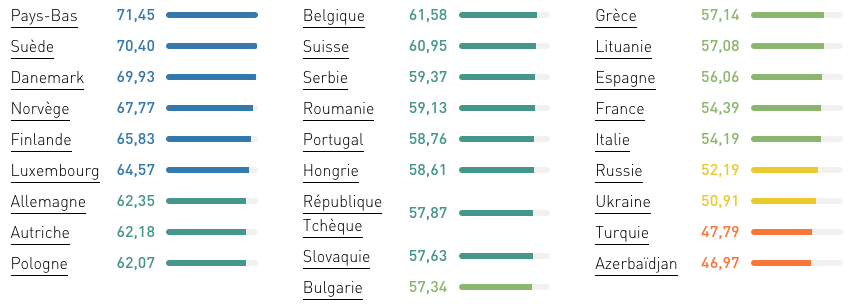
\includegraphics[scale=.5]{../img/french-english-level-in-europe}
    
    \label{fig:1}
  \end{figure}
\item niveau en anglais par rapport \href{http://doyouspeakenglish.fr/numero-1-en-tourisme-mais-dernier-en-anglais/}{au
    reste du monde}\footnote{Vous pouvez aller directement sur mon blog
  \url{http://doyouspeakenglish.fr/numero-1-en-tourisme-mais-dernier-en-anglais/} pour observer l'étude complète.}
(~derrière la République Dominicaine et la Corée du Sud s'il vous
plaît\ldots{} voir la figure \ref{fig:2} page \pageref{fig:2} pour
plus de détails~)
  \begin{figure}[h]
    \centering
    \caption[L'anglais dans le monde]{Niveau d'anglais dans le monde}\vspace{.1cm}
    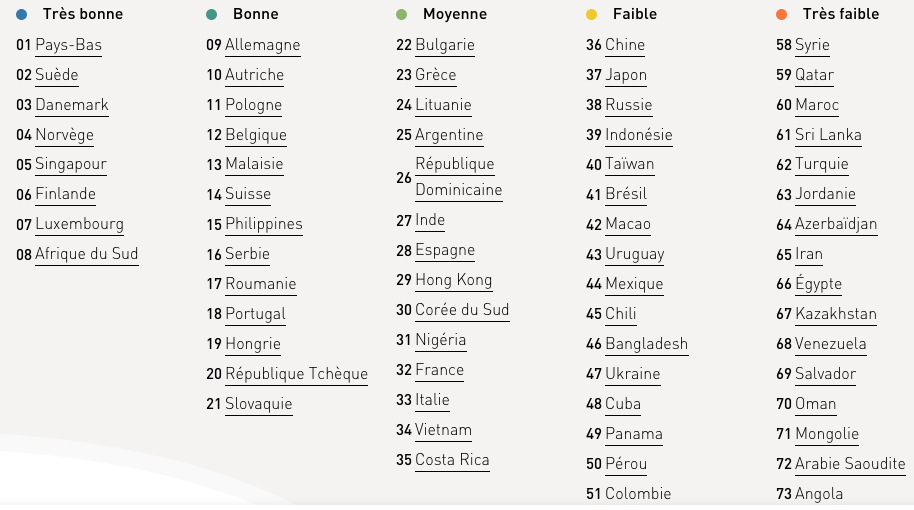
\includegraphics[scale=.5]{../img/english-level-in-the-world}
    
    \label{fig:2}
  \end{figure}
\item encore des
  \href{http://doyouspeakenglish.fr/les-francais-et-les-langues-en-quelques-chiffres/}{chiffres
    accablants}\footnote{Consulter mon article sur \url{http://doyouspeakenglish.fr/les-francais-et-les-langues-en-quelques-chiffres/}}
   
  \begin{figure}[h]
    \centering
    \caption[L'anglais en France]{Niveau d'anglais en France}\vspace{.1cm}
    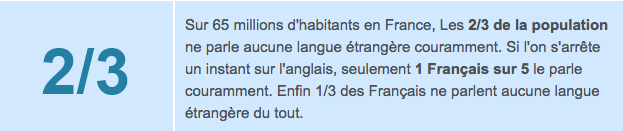
\includegraphics[scale=.725]{../img/french-english-level-in-france}
    
    \label{fig:3}
  \end{figure}
\end{itemize}
Loin de moi l'idée de vous assommer avec des chiffres et encore moins
de partir dans l'auto-flagellation. Néanmoins, il faut être lucide, il
y a un problème franco-français (~qui est très bien expliqué dans cet
\href{http://www.larevuedesressources.org/les-francais-et-les-langues-etrangeres,2920.html}{essai}~). 
Ce problème est très bien développé et analysé dans l'essai du
professeur Daniel Emilio Rojas\footnote{Lisez-le c'est gratuit, très
  bien écrit et instructif : \url{http://www.larevuedesressources.org/les-francais-et-les-langues-etrangeres,2920.html}} (~hispanophone natif qui parle et écrit
probablement beaucoup mieux le français que 90\% d'entre
nous~). Cependant, je me permettrais de vous proposer un raccourci\footnote{Forcément réducteur.} pédagogique en vous rappelant un fait
élémentaire mais que l'on oublie trop souvent. Parfois les solutions
sont tellement \underline{bêtes} qu'on oublie d'y penser. Attention, je ne
prétends pas vous proposer de recette miracle. L'anglais est une
langue difficile\footnote{Des linguistes professionnels et moi-même te
  le montrent dans cet article \url{http://doyouspeakenglish.fr/langlais-une-langue-facile/} }, bizarre, complexe et
illogique\footnote{Comme beaucoup de langues et notamment le
  français.}; et je ne suis pas le seul à le dire puisque certains anglophones natifs (~et
linguistes de surcroît~) le disent et l'écrivent par exemple dans cet \href{http://doyouspeakenglish.fr/langlais-une-langue-facile/}{article} qui permet également d'être
écouté\footnote{Comme je le montre dans cette vidéo
  \url{https://youtu.be/6wLbtx2iL7c}}. Donc oui l'anglais est
difficile, \underline{mais} avec un peu de bon sens et de persévérence
vous pouvez y arriver\footnote{Bon, il y a une triste vérité qu'il
  faut accepter, vous ne parlerez \underline{jamais} comme un natif (~\underline{sauf}
  si vous décidez de vous installer dans un pays anglophone~).}. 

\newpage
\section{Le truc tout bête}\label{sec:truc}
Mais quel est donc ce truc \underline{tout bête} que l'on oublierait et dont je
ne vous ai toujours pas parlé ? Minute papillon ! Non ! Je n'essaie
pas de noyer le poisson, je vais vous révéler mon \underline{truc}. Je vous
préviens, vous allez être probablement déçu, mais pourtant c'est une
évidence. \par
Allons-y ! Et bien, je ne sais pas pour vous mais pour moi\footnote{Et il me
semble pour la plupart des gens aussi.}, l'acquisition de ma langue
maternelle a commencé par l'oral et non par l'écrit. Pendant au moins
5 ans\footnote{Avant l'entrée au CP ou tout autre système scolaire qui
apprend à lire et à écrire.}, j'ai pratiqué en priorité l'écoute et la
méthode essai/erreur\footnote{En anglais on dit \exEN{try and guess} ce qui veut
dire \exFR{essayer et deviner}, qui est un point de vue plus positif (
attitude plus répandue chez les anglophones et en particulier chez les américains).}. Ben
oui, quand on est enfant on baigne dans un environnement linguistique
oral. Et dès les premiers mois de la vie on essaie (~avec beaucoup de
difficultés au début~) de produire ou plutôt reproduire des \textcolor{teal}{sons} que
l'on a entendu. Et croyez-moi, si vous avez oublié allez faire un tour
chez votre frère, soeur, cousin, cousine, ami, amie qui a (~ont~) des
enfants en bas âge et cela vous raffraichira la mémoire. La parole est
si importante pour l'humanité qu'elle a été pendant des siècles (~ des
millénaires même!~) le seul et unique vecteur de
communication. D'ailleurs aujourd'hui encore parmi les presque 7~000
\href{http://www.museedelhomme.fr/fr/combien-langues-sont-parlees-monde}{langues dans le monde} la plupart ne possèdent pas de système
d'écriture. Pour plus de précisions sur la répartition linguistique
dans le monde vous pouvez consulter \href{http://www.axl.cefan.ulaval.ca/Langues/1div\_recens.htm}{ce site canadien} qui tire ses
sources statistiques du \underline{Summer Institute of Linguistics} du
Texas\footnote{Voici l'url du site
  \url{http://www.axl.cefan.ulaval.ca/Langues/1div_recens.htm}}
(~2017~).\par

\newpage

\subsection{Quelques citations}\label{subsec:quote}

% \begin{bigquote}[1.0]
%   \begin{displayquote}[Extrait du livre \FL.][.]
%     Les Romains, déjà, ne parlaient pas exactement la langue qu'ils
%   écrivaient. Ainsi, \underline{cheval} vient d'un mot parlé,
%   \exLT{caballus}, alors que le latin classique écrit \exLT{equus} ---
%   d'où viendront des mots <<~savants~>> comme \underline{équidé} et
%   \underline{équitation}
%   \end{displayquote}
% \end{bigquote}  
        
\begin{center}
  \shadowbox{
    \begin{minipage}{\textwidth}
      {\fontfamily{Skia}\selectfont
        \blockquote[Extrait du livre \FL.][.]{%
          Les Romains, déjà, ne parlaient pas exactement la langue
          qu'ils écrivaient. Ainsi, \underline{cheval} vient d'un mot
          parlé, \exLT{caballus}, alors que le latin classique écrit
          \exLT{equus} --- d'où viendront des mots <<~savants~>> comme
          \underline{équidé} et \underline{équitation}%
        }
      }
    \end{minipage}%
  }
\end{center}

D'ailleurs comme le montre la première vidéo dans
\href{http://doyouspeakenglish.fr/prescriptiviste-ou-descriptiviste/}{cet
  article}, les zones du cerveau actives pour la parole et pour l'écriture sont différentes.\par

\begin{center}
  \shadowbox{
    \begin{minipage}{\textwidth}
      {\fontfamily{Skia}\selectfont
      \blockquote[Extrait du livre \FL.][.]{%
        Longtemps, le français s'est écrit comme il se parlait; vice versa,
        toutes les lettres se prononçaient, comme en latin. La notion même
        d'orthographe n'existait pas% 
      }%
      }
    \end{minipage}%
  }
\end{center}

En lisant ce dernier extrait je parie que certains d'entre vous sont en train
de chercher un moyen pour inventer une machine à remonter le temps. 

Vous vous demandez sûrement où je veux en venir. Mon but est de vous
faire comprendre ou plutôt de vous rappeler qu'une langue ça s'écoute
et ça se parle pendant un certain temps (~jusqu'à ce que ça devienne
naturel~) avant d'apprendre à l'écrire et d'étudier toutes les
subtilités de la grammaire. \href{https://fr.wikipedia.org/wiki/Django\_Reinhardt}{Django Reinhardt} et \href{https://fr.wikipedia.org/wiki/Louis\_Armstrong}{Louis Amstrong} ne
savaient ni lire ni écrire la musique et pourtant ils sont des
musiciens vénérés de leur vivant et encore aujourd'hui.\par

\newpage

\section{Une langue est une musique}\label{sec:music}
Et oui une langue c'est également une musique ! Une langue a une
musicalité et un rythme. Pas de chance pour nous le français (~ou
plutôt le \underline{parisien}\footnote{J'en parlerais plus en détails
  dans un prochain livre mais si vous êtes impatient alors je vous
  recommande de vous procurer \FL.}~)
n'est pas très chantant. Mais pourtant si l'on écoute les accents du
midi il y a tout de suite plus de mélodies qui chatouillent nos
oreilles. 

En résumé, ce que je vais partager avec vous dans ce livre, ce
sont les \textcolor{teal}{sons} de la langue anglaise. Les \href{https://pronunciationstudio.com/45-Sounds/}{45 \textcolor{teal}{sons}} (~certains en
décrivent 44, pour le français\footnote{Selon le \GE il y a 36 \textcolor{teal}{sons}
  <<~\exFR{purement}~>> français auquel on ajoute le \son~\phon{ŋ}
  hérité de l'anglais et notamment utilisé dans \exEN{parking}.} c'est
pareil, certains disent 36 d'autres 37~).\par

%\begin{itemize}
% \item Dans une première partie je vous présenterai la phonétique du
% français. En effet, il me semble plus judicieux d'approcher ce nouvel
% ensemble de symbole qui décrit les \textcolor{teal}{sons} avec précisément des \textcolor{teal}{sons} que
% vous utilisez déjà tous les jours.
Pour conclure cette introduction je rappelerai deux faits que l'on a tendance à oublier mais qu'il faut \underline{absolument garder à l'esprit} :

\begin{enumerate}
\item Le français est une langue syllabique alors que l'anglais est
  une langue accentuelle\footnote{Consulter mon \href{http://doyouspeakenglish.fr/laccent-tonique-en-anglais/}{article} de
    blog pour plus de détals.}.
\item En français il y a 36 \textcolor{teal}{sons}\footnote{Selon le
    \GE 36 mais selon Sousa auteur du livre \HTEBL il
    n'y en aurait que 32. Pour ce chiffre j'accorderai plus de crédit
    au \GE pour la bonne et simple raison qu'en tant que linguiste
    francophone il me semble plus compétant que Sousa qui est
    anglophone.} et 250 façons\footnote{Encore une fois les
    estimations diffèrent \GE n'en compte que 130 ce qui accentue
    encore plus la complexité de l'anglais.} de les écrire alors qu'en
  anglais il y a 44 \textcolor{teal}{sons} pour 1~100 façons de les écrire\footnote{Les
    chiffres concernant les façons d'écrire sont issus des
    comparaisons présentées dans le livre \HTEBL Chapter 4 Teaching
    English Language Reading and Writing page 84 Table 4.1.}.
\end{enumerate}

Par conséquent \underline{la prononciation, l'accent et le rythme} ne sont pas
superflus mais \underline{obligatoire en anglais}.\par

% Dans la deuxième partie du livre je vais vous présenter 45
% \textcolor{teal}{sons} qui sont absolument \underline{fondamentaux}
% dans la langue anglaise. En insistant particulièrement sur ceux qui
% n'apparaissent pas du tout dans la langue française.
% Et pour bien
% faire la différence il était important de commencer par la phonétique
% de la langue française que vous ne connaissez probablement pas
% encore. C'est pour cette raison qu'il est vivement recommandé de lire ce livre dans l'ordre.
%\end{itemize}

\newpage
\section{Mini conclusion de cette introduction}\label{sec:mini}
J'ai dit qu'on apprend d'abord à parler avant d'écrire, c'est vrai,
mais a priori, si vous lisez ce livre c'est que vous savez lire. Et
comme vous savez lire et bien on va en profiter pour apprendre encore
plus efficacement en utilisant
l'\href{https://fr.wikipedia.org/wiki/Alphabet_phon\%C3\%A9tique_international}{API}\CW{https://fr.wikipedia.org/wiki/Alphabet_phon\%C3\%A9tique_international}
(~Alphabet Phonétique International~). En anglais on l'écrit
IPA\CW{https://en.wikipedia.org/wiki/International_Phonetic_Alphabet}
(~International Phonetic Alphabet~).\par

Et cerise sur le gâteau, ceci
vous sera utile pour toutes les autres langues que vous souhaitez
apprendre ou que vous parlez déjà (~cela va même améliorer votre
français~). D'ailleurs, contrairement à ce que certaines personnes
pourraient penser, apprendre une autre langue, et en particulier
l'anglais, améliore votre niveau de français\footnote{En effet il existe plus de 25~000 mots anglais
  d'origine française et vous pouvez en découvrir quelques-uns grâce
  aux cartes mémoires que j'ai créé :
  \url{https://tinycards.duolingo.com/decks/6VNKUdba/english-words-with-french-origin}
et au livre plus complet \HSQMYP.}. Ce n'est pas magique,
mais c'est véridique. Alors c'est parti, allons découvrir les 45 \textcolor{teal}{sons}\footnote{Vous pouvez déjà vous entraîner grauitement grâce
  aux cartes mémoires que j'ai créé : \url{https://tiny.cards/decks/6YTEvyrN/english-phonetics}}
de la langue anglaise (~qui n'a plus grand chose à voir avec
Shakespeare de la même manière qu'on ne parle plus la langue de
Molière~).

\newpage
\minitoc


   \newpage
   \listoffigures
   \listoftables
   \newpage

   \mainmatter
   \parttoc

\part{Un peu de linguistique pour les non linguistes}

    \newpage
    \minitoc
    \newpage

    Bon, avant toute chose il est important de rappeler\footnote{Comme je
      l'avais déjà dit page~\pageref{sec:phonetics}.} que je ne suis pas
    un linguiste professionnel. À vrai dire, avant d'écrire ce livre on
    peut dire que je n'avais absolument aucune connaissance du sujet. Mais
    il se trouve que mon goût pour apprendre les langues étrangères m'a
    amené à approfondir la question. Et comme je n'ai pas envie de dire de
    bêtises je vais laisser la parole aux professionnels en me contentant
    de les citer, de les paraphraser et de vous transmettre ce que j'en ai
    compris. Par conséquent, celles et ceux qui voudraient aller plus loin
    sont vivement encouragés à le faire en se procurant les ouvrages cités
    qui sont très riches en informations. Pour les autres, il y a deux
    possibilités :
    
    \begin{enumerate}
    \item Vous n'avez pas envie d'apprendre de nouvelles choses théoriques
      et vous souhaitez directement passer à la pratique. Pas de problème
      ! Dans ce cas il vous suffit d'aller directement à la partie
      suivante page~\pageref{part:vow} pour les voyelles et
      page~\pageref{part:conson} pour les consonnes.
    \item Si comme moi vous aimez comprendre les choses sans forcément
      devenir un expert du domaine. Dans ce cas bienvenue dans cette
      partie où j'essaierai de vous communiquer la joie de la découverte
      et ma nouvelle passion pour ce domaine si riche et prometteur.  
    \end{enumerate}

    \begin{savequote}[80mm]
      \exEN{'Love all, trust a few, do wrong to none.'}
      \qauthor{\href{https://en.wikipedia.org/wiki/William_Shakespeare}{William Shakespeare}}
      \exFR{<<~Aimez tout le monde, faites confiance à quelques-uns, ne
        faites de mal à personne.~>>} 
      \qauthor{\href{https://fr.wikipedia.org/wiki/William_Shakespeare}{William Shakespeare}}
    \end{savequote}

    \chapter{Pourquoi la phonétique ?}\label{chap:phonetic}

\href{https://fr.wikipedia.org/wiki/Simon_Sinek}{Simon Sinek} qui est
un très bon motivateur explique très bien dans son livre
\href{https://amzn.to/2qY8uMD}{\exEN{Start with why}} que le
<<~Pourquoi ?~>> est la question fondamentale qu'il faut se poser en
premier. D'ailleurs, en parlant de Simon Sinek je vous recommande de
regarder cette \href{https://youtu.be/hER0Qp6QJNU}{vidéo} dans
laquelle il explique le problème des \exEN{millenials} (qu'on appelle
en français \exFR{la génération Y})\footnote{Et ce problème ne
  concerne pas uniquement les gens nés à partir des années 80, il concerne
  l'ensemble de la société.} et dans un registre légèrement je vous
recommande également mon article de blog sur ces sujets.  

\exEN{Why Phonetics?} est précisément le premier chapitre du livre
\lodge. Livre dont je vais vous proposer quelques extraits dans ce
chapitre. Extraits que nous analyserons et traduirons.

En voici un premier extrait :


\begin{center}
\begin{mdframed}[style=citestyle, frametitle={Extrait du livre \lodge}]
  \exEN{``The reasons for the study of phonetics should be made clear
      at the outset. This chapter is intended to set out the
      reasons why linguists (and any other people interested in
      spoken language of any kind) need phonetics as a tool of
      investigation.''}
\end{mdframed}
\end{center}
  

Ce qui donne en français :

\begin{center}
\begin{mdframed}[style=tradstyle, frametitle={\exFR{Traduction} de l'extrait ci-dessus}]
  \exFR{<<~Les raisons de l'étude de la phonétique devraient être
    précisées dès le départ. Ce chapitre vise à exposer les raisons
    pour lesquelles les linguistes (et toute autre personne intéressée
    par la langue parlée, quelle qu'elle soit) ont besoin de la
    phonétique comme outil d'investigation.~>>} 
\end{mdframed}  
\end{center}

Le ton est donné ! La phonétique est un outil nécessaire. Nous allons
explorer les explications que notre ami Lodge propose. Et je vous
recommande déjà vivement l'acquisition de son ouvrage.

\newpage
\minitoc
\newpage

\section{Comment décrivons-nous la parole ?}

Le titre de cette section est la traduction du titre de section de son
livre. Il est à noter que l'anglais n'a pas mot véritablement
équivalent au mot parole.

En effet, le titre original utilisait le mot \exEN{speech} qui sert
aussi à traduire le mot discours. En français aussi le mot discours
peut servir aussi bien pour l'écrit que pour l'oral.

Néanmoins le mot parole est plus précis commme nous le reverrons un
peu plus tard.

Revenons à notre section dont je vous propose un premier extrait ci-dessous pour commencer :

\begin{center}
\begin{mdframed}[style=citestyle, frametitle={Extrait du livre \lodge}]
  \exEN{''Traditional education largely ignores spoken language; even
    in drama and foreign language learning, little attention is paid
    to the details of speech in an objective way. We, therefore, need
    a method of describing speech in objective, verifiable terms, as
    opposed to the lay approaches which typically describe sounds as
    'hard', 'soft', 'sharp' and so on, which can only be properly
    understood by the person using such descriptions. Such an approach
    to any subject of study is totally subjective: since only the
    person carrying out the descriptions can understand them, other
    people are expected to be 'on the same wavelength' and clever
    enough to follow them. So, if we are to observe and describe
    speech in any meaningful way, we need some kind of objectively
    verifiable way of doing so. In fact, there are three ways of
    approaching the task.''}
\end{mdframed}  
\end{center}


La première partie de la première phrase est déjà éloquente avant même
que je vous livre la traduction vous avez déjà compris de quoi il
s'agit\dots{} l'oralité est ignorée, niée alors même qu'elle est le
fondement même du langage !

Observons désormais une traduction complète de cet extrait :

\begin{center}
\begin{mdframed}[style=tradstyle, frametitle={\exFR{Traduction} de l'extrait ci-dessus}]
    \exFR{L'éducation traditionnelle ignore en grande
    partie la langue parlée; même dans l'art dramatique et
    l'apprentissage des langues étrangères, peu d'attention est
    accordée aux détails de la parole d'une manière objective. Nous
    avons donc besoin d'une méthode de description de la parole en
    termes objectifs et vérifiables, opposés aux approches profanes qui
    décrivent généralement les sons comme ``durs'', ``doux'', ``forts'' et
    ainsi de suite, qui ne peut être correctement compris que par la
    personne utilisant de telles descriptions. Une telle approche pour
    n'importe quel sujet d'étude est totalement subjective : puisque
    seul la personne qui exécute les descriptions peut les comprendre,
    les autres sont censés être sur la même longueur d'onde et
    assez intelligents pour les suivre. Donc, si nous devons observer
    et décrire la parole de quelque manière significative, nous avons
    besoin d'un type de manière objectivement vérifiable de le
    faire. En fait, il y a trois façons d'approcher la tâche.} 
\end{mdframed}  
\end{center}


Que ceux qui trouvent que les mots sont un peu trop pompeux ou les
formules trop alambiquées se rassurent. Ce que notre ami Lodge nous
dit ici c'est tout simplement :
\begin{enumerate}
\item Que l'oralité a majoritairement toujours été considéré comme
  inférieure à l'écrit. Et c'est toujours le cas malheureusement. Il
  faut savoir que l'écriture est véritablement répandue que depuis
  l'invention de l'imprimerie. Et il faut attendre le 19ème siècle
  pour que le <<~peuple~>> accède à l'école et donc à la lecture et
  l'écriture. Par conséquent, l'oralité est ultra prépomdérante dans
  l'histoire de l'humanité y compris dans les pays où certains
  essaient d'imposer la supériorité de l'écrit. J'ajouterais que
  l'oralité est une prédisposition biologique ce qui n'est pas le cas
  de l'écrit. Et comme le dit très bien notre ami \href{https://youtu.be/1wsYbQxppRc}{Michel Serres}\footnote{\url{https://youtu.be/1wsYbQxppRc}},
  l'invention de l'écriture est une réduction de la mémoire ou plutôt
  une délégation de mémoire. Que ça soit la Bible ou les récits
  mythologiques Grecs\footnote{Ou d'ailleurs.}, la plupart des textes
  dits <<~sacrés~>> ont d'abord été des mémorisations
  orales\footnote{Ils n'avaient ni la télévision ni les réseaux
    sociaux du coup ils utilisaient davantages leurs réseaux
    neuronaux.}.
\item Que si l'on veut étudier le discours oral on a besoin d'outils
  objectifs. En effet, on ne peut pas se contenter d'expressions
  vagues comme les adjectifs cités dans son extrait. Qu'est-ce qu'un
  \son <<~dur~>> ? Dur à dire si j'ose le petit jeu de mot. Bien sûr
  c'est pratique lorsqu'on veut faire de l'art qui part essence est
  subjectif mais si l'on veut étudier scientifiquement la chose\dots{}
  et bien on a besoin d'une terminologie précise. En clair, notre ami
  Lodge nous dit que l'étude du discours oral doit être traitée comme
  toutes les autres sciences et pour ce faire il lui faut en quelques
  sorte une mathématisation ou si vous préférez une modélisation à
  l'aide de symboles précis.
\end{enumerate}

Voyons à présent quelles sont les trois façons qu'il décrit pour
s'atteler à cette tâche.

\newpage

\section{Première branche de la phonétique}\label{sec:phon-t1}

Commençons par la première branche de la phonétique.

\begin{center}
\begin{mdframed}[style=citestyle, frametitle={Extrait du livre \lodge}]
    \exEN{``What is speech exactly? The expression 'a lot of hot air' is
    rather a good starting point. Speech is made by modulating air in
    various ways inside our bodies. The organs of speech -- the lungs,
    throat, tongue, nose, lips and so on, which we shall discuss in
    detail in Chapter Two -- can be moved into many different
    configurations to produce the different sounds we perceive when
    listening to spoken language. A study of the ways in which these
    \textbf{articulators} of speech behave is called
    \textbf{articulatory phonetics}. In this book the detailed
    investigation of articulation will take up in eight out of the
    nine chapters.''}
\end{mdframed}  
\end{center}


Ce qui donne en français :

\begin{center}
\begin{mdframed}[style=tradstyle, frametitle={\exFR{Traduction} de l'extrait ci-dessus}]
  \exFR{Qu'est-ce que la parole ? L'expression ``beaucoup
    d'air chaud'' est plutôt un bon point de départ. La parole est
    faite en modulant l'air de diverses façons à l'intérieur de notre
    corps. Les organes de la parole -- les poumons, la gorge, la langue,
    le nez, les lèvres etc\dots{}, dont nous allons discuter
    en détail dans le chapitre deux -- peuvent être déplacés dans de
    nombreuses configurations différentes pour produire les différents
    sons que nous percevons quand nous écoutons la langue parlée. Une étude
    des façons dont ces \textbf{articulateurs} du discours se
    comportent est appelée \textbf{phonétique articulatoire}. Dans ce
    livre, l'enquête détaillée sur l'articulation occupera huit des
    neuf chapitres.}
\end{mdframed}  
\end{center}

De la même façon que notre ami Lodge l'a fait dans son livre, ici
aussi nous nous occuperons principalement de la phonétique
articulatoire. En bref, cela signifie que l'on va se focaliser sur la
façon de produire les sons. D'ailleurs, même si j'ai donné tous les
noms techniques, il n'est nullement question de théorie pour pratiquer
la phonétique et amélioration de sa prononciation, tout est question
d'écoute et de répétition. Mais comme l'a très justement souligné
notre ami Lodge, l'utilisation d'une terminologie précise a pour but
et avantage de nous permettre de nous y retrouver et de voir les
différences entre les sons.

Juste pour la culture poursuivons la description de notre ami Lodge. 

\newpage

\section{Deuxième branche de la phonétique}\label{sec:phon-t2}

Passons à la deuxième branche de la phonétique.

\begin{center}
\begin{mdframed}[style=citestyle, frametitle={Extrait du livre \lodge}]
  \exEN{``Basically, air is pushed out of the body and disturbs the outside
  air between the speaker and anyone in the vicinity who can hear
  him/her. These disturbances are known as \textbf{pressure
    fluctuations}, which in turn cause the hearer's eardrum to
  move. The molecules of the air move together and then apart in
  various ways, producing a \textbf{sound wave}. The study of the
  physical nature of sound waves is \textbf{acoustic
    phonetics}. We shall look at this aspect of speech and the
  relationship of articulation to acoustic effects in Chapter Nine.''}
\end{mdframed}  
\end{center}

    
Ce qui donne en français :

\begin{center}
\begin{mdframed}[style=tradstyle, frametitle={\exFR{Traduction} de l'extrait ci-dessus}]
  \exFR{Fondamentalement, l'air est expulsé du corps et perturbe
    l'air extérieur entre l'orateur et toute personne dans le
    voisinage qui peut l'entendre. Ces perturbations sont
    appelées \textbf{fluctuations de pression}, qui à leur tour
    provoquent le mouvement du tympan de l'auditeur. Les molécules de
    l'air se déplacent ensemble puis se séparent de diverses manières,
    en produisant une \textbf{onde sonore}. L'étude de la nature
    physique des ondes sonores est l'\textbf{acoustique
      phonétique}. Nous allons regarder cet aspect du discours et la 
    relation d'articulation aux effets acoustiques dans le chapitre neuf.}
\end{mdframed}  
\end{center}


Ceci est très intéressant et nous conduirait à une analyse physique du
\son qui serait également valable pour la musique. D'ailleurs, en
général, lorsqu'on parle d'acoustique la première chose qui vient à
l'esprit c'est la musique\footnote{À moins que je ne sois le seul à
  penser comme ça.}. Néanmoins, pour ce premier livre je me suis
restreint à la phonétique articulatoire. Et puis je vais vous faire
une petite confidence cette partie sur la linguistique est celle que
j'ai écrit en dernier parce que je me suis dit que faire une
introduction à la phonétique sans même la définir
sérieusement\footnote{Ben oui la petite définition Wikipédia c'est
  bien gentil mais c'est un peu léger.} ça serait un peu abuser. Du
coup ça m'a mis l'eau à la bouche pour un livre plus conséquent sur le
sujet. Mais pour l'instant mon approche est purement pragmatique,
comme utiliser ces outils pour améliorer et accélérer l'acquisition
d'une langue (ici l'anglais).

\newpage

\section{Troisième branche de la phonétique}\label{sec:phon-t3}

Observons maintenant la dernière branche de la phonétique.

\begin{center}
\begin{mdframed}[style=citestyle, frametitle={Extrait du livre \lodge}]
  \exEN{``The third way of considering speech, \textbf{auditory
      phonetics}, deals with the ways in which speech affects and is
    interpreted by the hearer(s). This aspect of the investigation of
    speech will not be considered in this book.''}
\end{mdframed}  
\end{center}

Ce qui donne en français :

\begin{center}
\begin{mdframed}[style=tradstyle, frametitle={\exFR{Traduction} de l'extrait ci-dessus}]
  \exFR{La troisième façon de considérer la parole, la
    \textbf{phonétique auditive}, traite des façons dont la
    parole affecte et est interprété par le ou les auditeur(s). Cet
    aspect de l'étude de la parole ne sera pas considéré dans ce livre.}
\end{mdframed}  
\end{center}


Maintenant je pense que vous avez un aperçu assez intéressant de ce
qu'est la phonétique. En particulier, même si nous nous restreindrons
à la phonétique articulatoire, il me semblait important de montrer la
rigueur scientifique qu'il y a derrière cette discipline qui ne se
résume pas aux pauvres petites transcriptions que l'on voit dans les
dictionnaires et dont les professeurs de langues ne nous ont jamais
parlé ni au collège ni au lycée.

Bien entendu notre cher ami Lodge ne s'adresse pas au
débutant\footnote{Encore qu'avec un peu de patience et de persévérance
tout le monde peut lire et comprendre son livre.}, je pense que sa
description est assez claire.

Nous en avons fini avec la description de la théorie phonétique. Avant
de rentrer dans le vif du sujet je vais tout de même faire un autre
petit chapitre similaire. Pourquoi ? Parce que l'autre source que j'ai
sélectionné est un manuel à l'usage de locuteurs non anglophones donc
son approche pourra nous être utile. Et de plus cette fois on brosse
un portrait général de la linguistique.

\newpage
\minitoc
\newpage



    \begin{savequote}[80mm]
      \exEN{"I don't focus on what I'm up against. I focus on my goals
        and I try to ignore the rest."}
      \qauthor{\href{https://en.wikipedia.org/wiki/Venus_Williams}{Venus
        Williams}}
      \exFR{<<~Je ne me concentre pas sur ce contre quoi je suis. Je
        me concentre sur mes objectifs et j'essaie d'ignorer le reste.~>>} 
      \qauthor{\href{https://fr.wikipedia.org/wiki/Venus_Williams}{Venus
          Williams}}
    \end{savequote}

    \chapter{La linguistique ça vous parle ?}\label{chap:linguistic}

La phonétique, normalement maintenant, vous savez à peu près ce que
c'est. Mais qu'en est-il de la linguistique ?

Ben il se retrouve que la phonétique en est une de ses branches.

\begin{center}
    \begin{figure}[h]
      \centering
        \begin{tikzpicture}
          \node {Linguistique}
          child { node {Phonétique}  
            child { node { articulatoire } }
            child { node { \dots } }
          }
          child { node {\dots} } 
          ;
        \end{tikzpicture}
    \caption{Branches de la linguistique}
    \label{fig:branch-phon}
  \end{figure}
\end{center}
Cela vous paraît peut être surprenant que je m'amuse à remonter les
branches. Pourtant c'est une démarche assez naturelle. On a
fondamentalement deux façons d'étudier un domaine.

\begin{enumerate}
\item La première consiste à partir du général  pour aller vers le
  particulier.
\item La seconde consiste à faire l'inverse.  
\end{enumerate}

 L'objet de ce livre étant de traiter de la phonétique anglaise il m'a
 paru plus opportun de démarrer avec une vue d'ensemble de la
 phonétique. Mais il me semble tout de même nécessaire de dessiner le
 contour de ce qu'est la linguistique qui, hélas, n'est pas une
 science très connue du grand public alors qu'elle est probablement la
 plus fondamentale.

 Au commencement était le verbe\footnote{Il est amusant de voir qu'en
   anglais ce n'est pas tout à fait pareil \exEN{In the beginning was
     the Word} qui se traduit littéralement par \exFR{Au commencement
     il y avait le Mot}.} aurait dit l'autre, et ce n'est pas pour
 rien, le langage oral est ce que nous partageons tous nous autres
 êtres humains. Quelle que soit votre activité, dans tous les cas vous
 communiquez par le langage.

 \'Etrangement à l'école nous ne l'étudions pas beaucoup ce
 langage. Lors des petites classes on nous fait apprendre les règles
 par c{\oe}ur puis on passe vite à la littérature (dès le collège) ou
 à la philosophie (au lycée). Il en va de même pour les langues
 étrangères. Pourtant lorsqu'on y réfléchi c'est tout de même étrange
 de se dire que nous partageons tous la même faculté de produire du
 langage mais que l'endroit où nous naissons va considérablement
 affecter les règles que nous allons utiliser pour le produire.

 Bref, sans plus attendre, laissons la parole aux professionnels que sont
 messieurs \textsc{Paul Burleigh} et \textsc{Peter Skandera} avec leur
 livre \href{https://amzn.to/2HV8BzG}{A Manual of English Phonetics and
  Phonology} qui était à la base destiné à un public de langue allemande.

\newpage
\minitoc
\newpage

\section{Prescriptivisme et descriptivisme}

Le débat entre prescriptivistes et descriptivistes est un éternel
débat dont j'avais déjà parlé dans cet
\href{http://doyouspeakenglish.fr/prescriptiviste-ou-descriptiviste/}{article}
de
blog\footnote{\url{http://doyouspeakenglish.fr/prescriptiviste-ou-descriptiviste/}}. Malheureusement
en France nous n'avons pas vraiment le droit de nous exprimer
puisqu'il existe une institution qui décide pour tout le monde des
règles de la langue française. Du coup, cela pourra paraître, au
premier abord, être une querelle de spécialiste. Mais il n'en est
rien, et ce serait une erreur de prendre ça à la légère ! C'est une
véritable question de fond !

\begin{center}
\begin{mdframed}[style=citestyle, frametitle={Extrait du livre \bs}]
  \exEN{``From ancient times until the present, language purists have
    believed that the task of the grammarian is to \emph{prescribe}
    (rather than \emph{describe}) correct usage that all educated
    people should use in speaking and
    writing. \textbf{Prescriptive} language scholars have
    laid down rules that are often based on Latin and Greek, on a
    classical canon of literary works, on the origin of particular
    words, on logic, or simply on their personal likes and
    dislikes. Prescriptivists have been criticised for not taking
    sufficient account of ongoing language change and stylistic
    variation. By contrast, the aim of linguistics is to
    \emph{describe} language objectively and
    systematically. \textbf{Descriptive} linguists observe
    and analyse language as it is used naturally in any given speech
    community [\emph{\textgerman{Sprachgemeinschaft}}], and they
    attempt to discover the rules and regularities of the underlying
    language system, or code.''}
\end{mdframed}  
\end{center}

Dès la première ligne on observe à quel point la question est
ancienne. Il est amusant de remarquer que le mot prescriptiviste a la
même racine que le verbe prescrire qui est utilisé par le médecin
lorsque nous sommes malades. Cela voudrait-il dire que certaines
personnes penseraient que d'autres sont malades de la langue ?

Occupons-nous désormais de la traduction.

\begin{center}
\begin{mdframed}[style=tradstyle, frametitle={\exFR{Traduction} d'un extrait du livre \bs}]
  \exFR{Depuis les temps anciens jusqu'à nos jours, les puristes de la
    langue croyaient que la tâche du grammairien est de \emph{prescrire}
(plutôt que \emph{décrire}) l'usage correct que tous les gens éduqués
devraient utiliser pour parler et écrire. Les professeurs de langues
\textbf{prescriptifs} ont établi des règles qui sont souvent
basées sur le latin et le grec, sur des canons classiques d'{\oe}uvres
littéraires, sur l'origine de certains mots, sur la logique, ou simplement sur
leurs goûts personnels en fonction de ce qu'ils aiment et n'aiment
pas. Les prescriptivistes ont été critiqués pour ne pas tenir compte
suffisamment du changement de la langue en usage et des variations
stylistiques. En revanche, le but de la linguistique est de
\emph{décrire} le langage objectivement et systématiquement. Les
linguistes \textbf{descriptivistes} observent et analysent
le langage tel qu'il est utilisé naturellement dans n'importe quel
discours donné dans une communauté
[\textgerman{\emph{Sprachgemeinschaft}}], et ils tentent de découvrir
les  règles et les régularités du système de langue sous-jacent, ou
code.}
\end{mdframed}  
\end{center}


Pour la faire simple on va dire que les prescriptivistes sont les
conservateurs et les descriptivistes les progressistes. Alors vu de
France c'est un peu compliqué parce que nous sommes fondamentalement
dans un pays prescriptiviste puisque une vieille bande d'illuminés
qui se prétendent immortels ont un droit absolu sur la façon de dicter
les lois de la langue française.

Bien heureusement, en France comme dans tous les pays, ce sont les
locuteurs qui font la langue et non les législateurs. Néanmoins ces
derniers ont tout de même un pouvoir fort sur la façon dont les
esprits sont éduqués. Et il est bien difficile de sortir du
conditionnement dont on a été victime durant son éducation il faut
bien le reconnaître.

Les linguistes étant par définition ceux qui observent et décrivent la
langue il serait intéressant d'en entendre parler avant de passer le
bac. Cela me semble plus concret et utile que de savoir que
Jean-Jacques\footnote{Ce même Jean-Jacques qui a écrit des choses
  beaucoup plus intéressantes comme le \href{https://www.rousseauonline.ch/pdf/rousseauonline-0004.pdf}{contrat social} par exemple.} s'est pris une fessée et l'a raconté dans son autobiographie\dots{}

\newpage
\section{Parole vs. langue et performance vs. compétence}

\begin{center}
\begin{mdframed}[style=citestyle, frametitle={Extrait du livre \bs}]
  \exEN{``In order to separate the two meanings of the word
    \emph{language} illustrated in the last sentence of the previous
    paragraph, the Swiss linguist Ferdinand de Saussure (1857-1913)
    proposed the French terms \textbf{parole} to refer to
    actual language use (i.e. to concrete utterances) and
    \textbf{langue} for a speech community's shared
    knowledge of a language (i.e. for the language system).''}  
\end{mdframed}  
\end{center}


Ce qui donne en français :

\begin{center}
\begin{mdframed}[style=tradstyle, frametitle={\exFR{Traduction} d'un extrait du livre \bs}]
  \exFR{Afin de séparer les deux significations du mot \emph{langage}
    illustré dans la dernière phrase du précédent paragraphe, le
    linguiste suisse Ferdinand de Saussure (1857-1913) proposa les
    termes français \textbf{parole} pour se référer à l'utilisation réelle
    de la langue (c'est-à-dire aux énoncés concrets) et
    \textbf{langue} pour un discours communautaire qui partage la
    connaissance d'une langue (c'est-à-dire pour le système
    linguistique).} 
\end{mdframed}  
\end{center}


On voit sur cet extrait que le français offre plus de précision grâce
aux mots parole, langue et langage là où l'anglais utilise
\exEN{speech} à la fois pour le discours écrit et oral ainsi que
\exEN{language} à la fois pour langue et langage. Il est important de
signaler également qu'à l'époque de Saussure, et ce jusqu'à la seconde
guerre mondiale, le français était la \exLT{lingua franca}, la langue
dominante, la langue noble. Rôle joué par l'anglais désormais. 

\begin{center}
\begin{mdframed}[style=citestyle, frametitle={Extrait du livre \bs}]
  \exEN{``A similar dichotomy was put forward by the American linguist
    Noam Chomsky (b. 1928), who used the terms \textbf{performance}
    and \textbf{competence} to refer to largely the same
    concepts. Chomsky, however, put more emphasis on the individual
    nature of language. Performance, then, is the actual language use
    of an individual speaker, and competence is that individual
    speaker's knowledge of the language. Chomsky later replaced these
    terms with \textbf{E(xternalised)-language} and
    \textbf{I(nternalised)-language}, but the new terms are rarely used.''}  
\end{mdframed}  
\end{center}

Ce qui donne en français :

\begin{center}
\begin{mdframed}[style=tradstyle, frametitle={\exFR{Traduction} d'un extrait du livre \bs}]
  \exFR{Une dichotomie similaire a été mise en avant par le linguiste
    américain Noam Chomsky (né en 1928), qui utilisait les termes
    \textbf{performance} et \textbf{compétence} pour se référer
    largement aux mêmes concepts. Chomsky, cependant, met plus l'accent
    sur la nature individuelle de la langue. La performance, alors, est
    l'utilisation réelle de la langue d'un locuteur individuel, et la
    compétence est la connaissance personnelle du locuteur de la
    langue. Chomsky a plus tard remplacé ces termes avec \textbf{langue
      (E)xternalisée} et \textbf{langue I(nternalisée)}, mais les
    nouveaux termes sont rarement utilisés.}   
\end{mdframed}  
\end{center}


Là on commence à s'aventurer sur un domaine plus technique donc je
n'irais pas plus loin dans la profondeur. J'ai cité ce passage car
Noam Chomsky est le scientifique qui a le plus contribué dans le
domaine de la linguistique. Par conséquent il était très important de
citer au moins un de ses apports. La section suivante sera plus
intéressante du point de vue de la vulgarisation.

\newpage

\section{Les quatre domaines de base de la linguistique}

Voyons à présent les quatre branches majeures de la linguistique de
base, telle qu'elle a été conçue à son origine.

\begin{center}
\begin{mdframed}[style=citestyle, frametitle={Extrait du livre \bs}]
  \exEN{``The system or structure of a language (langue or competence)
    can be described at four different levels, which form the core
    areas of linguistics, sometimes called \emph{microlinguistics}:
    (1) \textbf{Phonetics} and \textbf{phonology} deal with
    pronunciation, or, more precisely, with speech sounds and the
    sound system. (2) \textbf{Morphology} covers the structure of
    words. (3) \textbf{Syntax} explains sentence patterns. (Morphology
    and syntax, often combined into \emph{morphosyntax}, have
    traditionally been referred to as \emph{grammar}.) (4)
    \textbf{Lexicology} and \textbf{semantics} describe the
    vocabulary, or lexicon, and explore different aspects of meaning.''}  
\end{mdframed}  
\end{center}

Derrière ces noms qui peuvent éventuellement faire peur se cache des
opérations\footnote{En ce sens la linguistique est véritablement très
  proche des mathématiques, d'ailleurs en informatique théorique
  l'arithmétique est considérée comme un langage avec un alphabet à 10
symboles si on utilise le système décimal par exemple.} que l'on fait
instinctivement.

Par exemple pour la phonétique et la phonologie du français nous
n'avons pas eu besoin de les théoriser car nous les avons appris
empiriquement par écoute et imitation des sons.

Il en va de même pour la formulation des mots (morphologie); d'ailleurs je suis sûr
qu'il vous est déjà arrivé d'inventer des mots avant même de savoir
lire ou écrire.

Pour ce qui est de la syntaxe c'est un peu plus délicat mais pour ce
qui est des phrases de base elles se construisent également
instinctivement. C'est précisément sur la syntaxe que les esprits
chagrins revendiquent le prescriptivisme.


Passons maintenant à la traduction :

\begin{center}
\begin{mdframed}[style=tradstyle, frametitle={\exFR{Traduction} d'un extrait du livre \bs}]
  \exFR{Le système ou la structure d'une langue (langue ou compétence)
    peut être décrit à quatre niveaux différents, qui forment le
    c{\oe}ur des domaines de la linguistique, parfois appelé
    \emph{microlinguistique}: (1) La \textbf{phonétique} et la
    \textbf{phonologie} traitent de la prononciation, ou, plus
    précisément, des sons de la parole et du système auditif. (2)
    La \textbf{morphologie} couvre la structure des mots. (3) La
    \textbf{syntaxe} explique les modèles de phrases. (Morphologie et
    syntaxe, souvent combinées en \emph{morphosyntaxe}, ont
    traditionnellement été dénommé \emph{grammaire}.) (4) La
    \textbf{lexicologie} et la \textbf{sémantique} décrivent le
    vocabulaire, ou lexique, et explorent différents aspects de la
    signification.}    
\end{mdframed}  
\end{center}


À présent nous avons une vue d'ensemble qui me semble assez
claire.

Finalement, selon moi, la linguistique traite véritablement de
la façon dont nous communiquons.

En partant de la façon dont nous produisons et recevons les sons
(c'est précisément le rôle de la phonétique et de la phonologie).

Puis elle analyse la façon dont nous construisons les mots (la
morphologie) et les phrases (la syntaxe) par ajacement de ces
derniers.

Enfin, nos communications ont un sens (la sémantique).

Il est véritablement curieux que la linguistique ne soit pas enseignée
dès le plus jeune âge car c'est véritablement l'outil le plus
important que tout être humain devrait maîtriser ou du moins connaître les bases.

J'arrête ici avec les citations mais je vous dresse tout de même
brièvement la liste des autres branches de la linguistique (qu'on
appelle la \emph{macrolinguistique} afin d'aiguiser votre curiosité
car vous allez voir cela touche à de nombreux domaines. Notamment des
domaines qui concernent les nouvelles technologies.

\begin{enumerate}
\item La \textbf{dialectologie} qui est l'intersection entre la
  linguistique et la géographie. Par exemple en anglais cela
  consisterait à se pencher sur les variations entre les différentes
  variations selon que l'on est en Angleterre, en \'Ecosse, au
  Canada\dots{} ou ailleurs.
\item La \textbf{socio-linguistique} qui comme son nom l'indique mêle
  sociologie et linguistique. Si l'on reprend l'exemple de l'anglais
  on pourrait par exemple étudier le fait que l'accent RP était une
  façon de montrer son appartenance à une classe sociale élevée.
\item L'\textbf{ethno-linguistique} qui est à la frontière entre
  l'anthropologie, l'ethnologie et la linguistique. On peut voir que les
  trois premiers domaines sont assez proches.
\item L'\textbf{analyse du discours}, la \textbf{linguistique
    textuelle} et \textbf{stylistique} s'occuppent cette fois des
  variations au niveau supérieur que les phrases. Pour l'oral par
  exemple cela va consister à analyser des conversations, des
  discours, des conférences et ainsi de suite. Concernant l'écrit, on
  étudiera les lettres personnelles, les articles de presse, ou encore
  les papiers universitaires.
\item La \textbf{linguistique comparative} décrit les similarités et
  différences entre des langues modernes. Par exemple entre l'anglais
  et le français.
\item La \textbf{psycholinguistique} à cheval entre la psychologie et
  la linguistique. Elle s'intéresse notamment à l'apprentissage.
\item La \textbf{neurolinguistique} qui s'occupe des connexions entre
  le langage et le système nerveux.
\item La \textbf{linguistique computationnelle} qui est probablement
  la plus récente et qui connaît un essor considérable grâce à
  l'avènement des nouvelles technologies et en particulier
  l'intelligence artificielle. C'est dans cette branche de la
  linguistique que l'on s'occupe du traitement automatique des langues
  comme par exemple les outils de traduction automatique en ligne ou
  sur application mobile ou encore les outils de reconnaissance
  vocale.   
\end{enumerate}

Comme vous avez dû vous en rendre compte la linguistique couvre
potentiellement l'ensemble du spectre des connaissances humaines. Je
vous avouerais que je suis particulièrement sensible à la dernière
branche citée. J'espère vous avoir communiqué mon appétit pour la
découverte de ce champ d'investigation aussi vaste qu'intéressant et
je vous invite désormais à vous concentrer sur la
phonétique\footnote{À partir de maintenant je ne parlerai que de la
  phonétique articulatoire parce que c'est celle que l'on trouve dans
  les dictionnaires et que nous pratiquons lorsque nous produisons les
  sons.}, et en particulier celle de l'anglais.

\begin{center}
  \begin{figure}[h]
    \centering
    \includegraphics[scale=.65]{../img/burleigh-skandera/app-phon-bs}
    \caption{Organes de la parole, issu du livre \bs}
    \label{fig:app-phon}
  \end{figure}
\end{center}

Je vous souhaite une bonne étude à l'aide de ce guide.

\newpage
\minitoc


    
\part{Vowel sounds}\label{part:vow}

    
    J'attire votre attention sur 2 points importants afin d'éviter toute
    confusion :

    \begin{enumerate}
    \item D'une part, en anglais il n'y a que 5 voyelles écrites :
      \exEN{a}, \exEN{e}, \exEN{i}, \exEN{o} et \exEN{u}, et non pas 6
      comme en \exFR{français}, parce que le \exEN{y} n'est pas  considéré
      comme une voyelle écrite par les anglophones.
    \item D'autre part, en phonétique on s'intéresse aux sons et non pas aux
      lettres, par conséquent lorsqu'on parlera de voyelle cela
      sous-entendra toujours\footnote{Sauf mention explicite du
        contraire.} que l'on parle de \underline{voyelle sonore}. En
      effet, la phonétique étant la science de la production sonore du
      langage cela ne ferait pas sens de s'intéresser aux lettres qui sont
      indépendantes de la physique du son et de la biologie de notre anatomie.
    \end{enumerate}

    Selon
    \href{https://fr.wikipedia.org/wiki/Phon\%C3\%A9tique}{Wikipédia}
    :
    
    \begin{quote}
      La phonétique (du grec « phônê » qui signifie la « voix », le «
      son ») est une branche de la linguistique qui étudie les sons
      utilisés dans la communication parlée. À la différence de la
      phonologie, qui étudie comment sont agencés les phonèmes d'une
      langue pour former des mots, la phonétique concerne les sons
      eux-mêmes (les unités phonétiques, les « phones »), leur
      production, leur variation plutôt que leur contexte. La
      sémantique ne fait donc pas partie de ce niveau d'analyse linguistique.
    \end{quote}

    Un \textcolor{teal}{son} de
    \textcolor{teal}{voyelle}\CW{https://en.wikipedia.org/wiki/English_phonology\#Vowels} 
    est fait en façonnant l'air comme il quitte la bouche. Nous
    utilisons les articulateurs pour façonner l'air --- les lèvres, la
    mâchoire, la langue. L'\exEN{anglais} britannique utilise 12
    positions de la bouche\footnote{Vous pouvez les voir et les
      entendre en consultant ce
      \href{https://pronunciationstudio.com/vowel02/}{site}.}.   

    Pour accéder à une banque de \textcolor{teal}{sons} de
    \textcolor{teal}{voyelles} avec la figure~\ref{fig:ipa-vowels} ci-dessous rendez-vous sur
    la page \url{https://en.wikipedia.org/wiki/Vowel\#Audio_samples}.

    \begin{center}
      \begin{figure}[h]
        \centering
        \includegraphics[scale=.5]{../img/IPA_vowel_chart_2005}
        \caption{\href{https://en.wikipedia.org/wiki/Vowel\#Audio_samples}{\exEN{IPA Vowels}}}
        \label{fig:ipa-vowels}
      \end{figure}
    \end{center}

    \begin{savequote}[80mm]
      \exEN{"Great things in business are never done by one
        person. They're done by a team of people."}
      \qauthor{\href{https://en.wikipedia.org/wiki/Steve_Jobs}{Steve Jobs}}
      \exFR{<<~Les grandes choses dans les affaires ne sont jamais
        faites par une personne. Elles sont faites par une équipe de gens.~>>} 
      \qauthor{\href{https://fr.wikipedia.org/wiki/Steve_Jobs}{Steve Jobs}}
    \end{savequote}
    
    \chapter{Front Vowels (langue vers l'avant)}\label{chap:frontvow}

\speech{4}{voyelles antérieures\CW{https://fr.wikipedia.org/wiki/Voyelle_ant\%C3\%A9rieure}}

\begin{center}
  \begin{figure}[h]
    \centering
    \includegraphics[scale=.75]{../img/Esling_vowel_chart.png}
    \caption[\exEN{Front
     Vowels}]{\exEN{Front
          Vowels}, Source : \href{https://en.wikipedia.org/w/index.php?curid=46937434}{Wikipedia}}
    \label{fig:front-vowels}
  \end{figure}
\end{center}

\newpage
\minitoc
\newpage

\section{Le \son \phon{iː}}\label{sec:ilong}

\hypertarget{ilong}{Ce \son} a pour nom technique\dyse{clear-front-unrounded-vowel} :

\begin{itemize}
\item \exEN{Close Front Unrounded Vowel\CW{https://en.wikipedia.org/wiki/Close_front_unrounded_vowel}.}
\item \exFR{Voyelle fermée antérieure non arrondie\CW{https://fr.wikipedia.org/wiki/Voyelle_ferm\%C3\%A9e_ant\%C3\%A9rieure_non_arrondie}.}
\end{itemize}

\begin{center}
  \begin{figure}[h]
    \centering
    \includegraphics{../img/non-arrondies-wikipedia.png}
    \caption{Voyelles non-arrondies, source : Wikipédia}
    \label{fig:voy-ferm}
  \end{figure}
\end{center}

\indicsound

\properukus{https://youtu.be/EuZa9-QbhG8}{https://youtu.be/PIu5WDIco0I}

\begin{enumerate}
\item \exEN{\href{http://www.wordreference.com/enfr/need}{need}} qui s'écrit en \gls{phon} \href{https://en.oxforddictionaries.com/definition/need}{\phonm{niːd}}

  \begin{itemize}
  \item\exEN{I \href{https://youtu.be/p0quLJutRC8}{need} to work every day if I want to \href{https://www.youtube.com/watch?v=xqMozc4K4pg&list=PLE_vQWWxgaiHUFB8zsbcEYqJL0GHGdMLi}{improve} my level.}
  \item\exFR{Je dois travailler tous les jours si je veux
      améliorer mon niveau.}
  \end{itemize}

  \youglish{need}


\item \exEN{\href{http://www.wordreference.com/enfr/tea}{tea}} qui s'écrit en \gls{phon} \href{https://en.oxforddictionaries.com/definition/tea}{\phonm{tiː}}

  \begin{itemize}
  \item\exEN{\href{https://youtu.be/S8SdWEQg6cE}{Every morning} we are
      used to drinking \href{https://youtu.be/Euh8dY4EU9o}{tea}.}
  \item\exFR{Tous les matins on a l'habitude de boire du thé.}
  \end{itemize}

  \youglish{tea}

\item \exEN{\href{http://www.wordreference.com/enfr/believe}{believe}}
  qui s'écrit phonétiquement
  \href{https://en.oxforddictionaries.com/definition/believe}{\phonm{bɪˈliːv}}
  
  \begin{itemize}
  \item\exEN{\href{https://youtu.be/GIQn8pab8Vc}{I believe I can fly.}}
  \item\exFR{Je crois que je peux voler.}
  \end{itemize}

  \youglish{believe}
  
\item \exEN{\href{http://www.wordreference.com/enfr/see}{see}} qui s'écrit
  phonétiquement
  \href{https://en.oxforddictionaries.com/definition/see}{\phonm{siː}}
  
  \begin{itemize}
  \item\exEN{What You \href{https://youtu.be/Dpf2yHjBVYM}{See} Is What You Get (\href{https://fr.wikipedia.org/wiki/What\_you\_see\_is\_what\_you\_get}{WYSIWYG})}
  \item\exFR{Ce que vous voyez est ce que vous obtenez.}
  \end{itemize}

  \youglish{see}
  
\end{enumerate}
\newpage

\section{Le \son \phon{ɪ}}\label{sec:soni}

\hypertarget{soni}{Ce \son} a pour nom technique\dyse{near-close-near-front-unrounded-vowel} :

\begin{itemize}
\item \exEN{Near-Close Near-Front Unrounded Vowel\CW{https://en.wikipedia.org/wiki/Near-close_near-front_unrounded_vowel}.}
\item \exFR{Voyelle pré-fermée antérieure non arrondie\CW{https://fr.wikipedia.org/wiki/Voyelle_pr\%C3\%A9-ferm\%C3\%A9e_ant\%C3\%A9rieure_non_arrondie}.}
\end{itemize}

\begin{center}
  \begin{figure}[h]
    \centering
    \includegraphics{../img/non-arrondies-wikipedia.png}
    \caption{Voyelles non-arrondies, source : Wikipédia}
    \label{fig:voy-ferm}
  \end{figure}
\end{center}

\indicsound

\properukus{https://youtu.be/7PpuPMrISVc}{https://youtu.be/Ok_HG-0lNCA}

\begin{enumerate}
\item \exEN{\href{http://www.wordreference.com/enfr/england}{England}} qui s'écrit en \gls{phon} \href{https://en.oxforddictionaries.com/definition/england}{\phonm{ˈɪŋɡlənd}}

  \begin{itemize}
  \item\exEN{Last \href{https://youtu.be/j9xSxJRsmx0}{summer} I went to \href{https://youtu.be/QUPBesOdax8}{England}.}
  \item\exFR{L'été dernier je suis allé en Angleterre.}
  \end{itemize}

  \youglish{England}
  
\item \exEN{\href{http://www.wordreference.com/enfr/thin}{thin}} qui s'écrit en \gls{phon} \href{https://en.oxforddictionaries.com/definition/thin}{\phonm{θɪn}}

  \begin{itemize}
  \item\exEN{Usually \href{https://youtu.be/IpRSyVcHu-k}{top models} are \href{https://youtu.be/LekA62H17bo}{thin}.}
  \item\exFR{Habituellement les mannequins sont minces.}
  \end{itemize}

  \youglish{thin}
  
\item \exEN{\href{http://www.wordreference.com/enfr/big}{big}} qui s'écrit phonétiquement \href{https://en.oxforddictionaries.com/definition/big}{\phonm{bɪɡ}}

  \begin{itemize}
  \item\exEN{\href{https://youtu.be/do7w0j4ybeY}{New York} has a nickname: the \href{https://youtu.be/Jha4OkG-ixw}{Big} Apple.}
  \item\exFR{New York a un surnom : la grosse pomme.}
  \end{itemize}

  \youglish{big}
  
\item \exEN{\href{http://www.wordreference.com/enfr/which}{which}} qui s'écrit phonétiquement \href{https://en.oxforddictionaries.com/definition/which}{\phonm{wɪtʃ}}

  \begin{itemize}
  \item\exEN{\href{https://youtu.be/DN74ZuSrtxY}{Pick up} a glass from the table. \href{https://youtu.be/5fR\_\_LXDkRg}{Which} one?}
  \item\exFR{Choisis un verre sur la table. Lequel ?}
  \end{itemize}

  \youglish{which}
  
\end{enumerate}
\newpage

\section{Le \son \phon{ɛ}  parfois noté \phon{\href{https://dictionary.cambridge.org/dictionary/english/bed}{e}}
  }\label{sec:sone}

Il est important de préciser que le \son \phon{e} n'existe pas en anglais
pour la bonne et simple raison que ce symbole \gls{phon} représente le
<<~\exFR{é}~>> comme dans le mot français \exFR{beauté}. Je n'ai pas réussi à
trouver d'explication suffisamment détaillée si ce n'est une <<~raison
historique~>> évoquée sur une page de
\href{http://teflpedia.com/IPA_phonetic_symbol_\%E3\%80\%9A\%C9\%9B\%E3\%80\%9B}{teflpedia}\footnote{Teflpedia
est un site inspiré de Wikipédia consacré au TEFL: Teaching English as
a Foreign Language (Enseignement de l'Anglais comme Langue \'Etrangère
équivalent du FLE : Français Langue \'Etrangère).}.

\begin{center}
  \begin{figure}[h]
    \centering
    \includegraphics[scale=.75]{../img/teflopedia-tab-1}
    \caption[Quel symbole \gls{phon} pour le son <<~\exFR{è}~>>]{Démocratiquement
      la notation \textcolor{teal}{[ɛ]} est préférable à l'ancienne \textcolor{teal}{[e]}}
    \label{fig:teflpedia-1}
  \end{figure}
\end{center}

Paradoxalement, alors que le tableau de la
figure~\ref{fig:teflpedia-1} montre clairement que la majorité des
dictionnaires utilisent à raison le symbole \textcolor{teal}{[ɛ]},
ils\footnote{teflpedia} font partie de la minorité qui persite à
utiliser le symbole \textcolor{teal}{[e]}. Ceci est un problème pour
nous autres francophones parce que ce symbole \textcolor{teal}{[e]}
nous sert à représenter le son <<~\exFR{é}~>> qui n'existe pas en
anglais. Ce détail est \underline{très important} parce que le but de
l'API est précisément de fournir un alphabet international afin que
tous les \glspl{linguist} (et les utilisateurs de la \gls{phon}) puissent se 
comprendre. Cet ensemble de symboles ne sert pas uniquement pour
apprendre à prononcer l'anglais. Il est valable pour toutes les
langues humaines (y compris celles qui n'ont pas d'alphabet). Alors je
trouve ça très dérangeant qu'un groupe qui a vocation à enseigner
l'anglais aux étrangers persiste à maintenir la confusion. Hélas, ils
ne sont pas les seuls et certains manuels faits par des francophones
pour des francophones perpétuent l'erreur\footnote{Ce qui est d'autant
  plus blâmable puisqu'il s'agit d'une négation de la phonétique
  française !}.

\notation

\hypertarget{sone}{Ce \son} a pour nom technique\dyse{open-mid-front-unrounded-vowel} :

\begin{itemize}
\item \exEN{Open-Mid Front Unrounded Vowel\CW{https://en.wikipedia.org/wiki/Open-mid_front_unrounded_vowel}.}
\item \exFR{Voyelle mi-ouverte antérieure non arrondie\CW{https://fr.wikipedia.org/wiki/Voyelle_mi-ouverte_ant\%C3\%A9rieure_non_arrondie}.}
\end{itemize}

\begin{center}
  \begin{figure}[h]
    \centering
    \includegraphics{../img/non-arrondies-wikipedia.png}
    \caption{Voyelles non-arrondies, source : Wikipédia}
    \label{fig:voy-ferm}
  \end{figure}
\end{center}

\indicsound

\properukus{https://youtu.be/JhBH_rtOXGA}{https://youtu.be/xKxV8XfigaE}

\begin{enumerate}
\item \exEN{\href{http://www.wordreference.com/enfr/bed}{bed}} qui s'écrit
  phonétiquement
  \href{https://en.oxforddictionaries.com/definition/bed}{\phonm{bɛd}}

  \begin{itemize}
  \item\exEN{\href{https://youtu.be/LnshfLOhr2Q}{It's time to go} to \href{https://youtu.be/urARKkLo6MY}{bed}.}
  \item\exFR{C'est l'heure d'aller se coucher.}
  \end{itemize}

  \youglish{bed}
  
\item \exEN{\href{http://www.wordreference.com/enfr/bread}{bread}} qui s'écrit phonétiquement \href{https://en.oxforddictionaries.com/definition/bread}{\phonm{brɛd}}
  
  \begin{itemize}
  \item\exEN{\href{https://youtu.be/yxgE3ifjZ94}{French people} are famous for their \href{https://youtu.be/Ynm9Wrznz4I}{bread}.}
  \item\exFR{Les Français sont célèbres pour leur pain.}
  \end{itemize}

  \youglish{bread}
  
\item \exEN{\href{http://www.wordreference.com/enfr/said}{said}} qui s'écrit
  phonétiquement
  \href{https://en.oxforddictionaries.com/definition/said}{\phonm{sɛd}}

  \begin{itemize}
  \item\exEN{\href{https://www.azlyrics.com/lyrics/beatles/yesterday.html}{Yesterday} you said that \href{https://youtu.be/9IDogHTQgM4}{same thing}.}
  \item\exFR{Hier tu as dit cette même chose.}
  \end{itemize}

  \youglish{said}
  
\item \exEN{\href{http://www.wordreference.com/enfr/friend}{friend}} qui
  s'écrit phonétiquement
  \href{https://en.oxforddictionaries.com/definition/friend}{\phonm{frɛnd}}

  \begin{itemize}
  \item\exEN{\href{https://youtu.be/q-9kPks0IfE}{I'll be there for you} my \href{https://youtu.be/CY8E6N5Nzec}{friend}.}
  \item\exFR{Je serais là pour toi mon ami(e).}
  \end{itemize}

  \youglish{friend}
  
\end{enumerate}
\newpage

\section{Le \son \phon{æ} noté aussi parfois
\phon{\href{https://en.oxforddictionaries.com/definition/cat}{a}}
  }\label{sec:sonae}

  \notation
  
\hypertarget{sonae}{Ce \son} a pour nom technique\dyse{near-open-front-unrounded-vowel} :

\begin{itemize}
\item \exEN{Near-Open Front Unrounded Vowel\CW{https://en.wikipedia.org/wiki/Near-open_front_unrounded_vowel}.}
\item \exFR{Voyelle ouverte antérieure non arrondie\CW{https://fr.wikipedia.org/wiki/Voyelle_pr\%C3\%A9-ouverte_ant\%C3\%A9rieure_non_arrondie}.}
\end{itemize}

\begin{center}
  \begin{figure}[h]
    \centering
    \includegraphics{../img/non-arrondies-wikipedia.png}
    \caption{Voyelles non-arrondies, source : Wikipédia}
    \label{fig:voy-ferm}
  \end{figure}
\end{center}

\indicsound

\properukus{https://youtu.be/NavmTDkd8Z8}{https://youtu.be/mynucZiy-Ug}

\begin{enumerate}
\item \exEN{\href{http://www.wordreference.com/enfr/bat}{bat}} qui s'écrit
  phonétiquement
  \href{https://dictionary.cambridge.org/dictionary/english/bat}{\phonm{bæt}}
  
  \begin{itemize}
  \item\exEN{Have you ever noticed that \href{https://youtu.be/ulOLYnOthIw}{Batman} means the \href{https://youtu.be/WfGMYdalClU}{man} who
      is a \href{https://youtu.be/eozL5n2Plmc}{bat}?}
  \item\exFR{As-tu déjà remarqué que Batman signifie l'homme qui
      est une chauve-souris ?}
  \end{itemize}

  \youglish{bat}
  
\item \exEN{\href{http://www.wordreference.com/enfr/cat}{cat}} qui s'écrit
  phonétiquement
  \href{https://dictionary.cambridge.org/dictionary/english/cat}{\phonm{kæt}}

  \begin{itemize}
  \item\exEN{What \href{https://youtu.be/7FjChUY0zgQ}{about} Catwoman? Is she a \href{https://youtu.be/eNQazP-wdj4}{cat}?}
  \item\exFR{Qu'en est-il de Catwoman ? Est-elle une chatte ?}
  \end{itemize}

  \youglish{cat}
  
\item \exEN{\href{http://www.wordreference.com/enfr/that}{that}} qui s'écrit phonétiquement \href{https://dictionary.cambridge.org/dictionary/english/that}{\phonm{ðæt}} 
\begin{itemize}
\item\exEN{\href{https://youtu.be/HAlz5TiKOCM}{That} house is \href{https://youtu.be/qYvXk_bqlBk}{really} big.}
\item\exFR{Cette maison est vraiment grande.}
\end{itemize}

\youglish{that}

\item \exEN{\href{http://www.wordreference.com/enfr/hand}{hand}} qui s'écrit
  phonétiquement
  \href{https://dictionary.cambridge.org/dictionary/english/hand}{\phonm{hænd}}

  \begin{itemize}
  \item\exEN{\href{https://youtu.be/-ccNkksrfls}{Maradona} scored with his \href{https://youtu.be/KDKBY9FqwQg}{hand} during a famous
      match between Argentina and England.}
  \item\exFR{Maradona avait marqué avec sa main durant un célèbre
      match entre l'Argentine et l'Angleterre.}
  \end{itemize}

  \youglish{hand}
  
\end{enumerate}

\begin{center}
  \begin{figure}[h]
    \centering
    \includegraphics[scale=.75]{../img/Cardinal_vowel_tongue_position-front.svg.png}
    \caption[\exEN{Idealistic Tongue Positions}]{\exEN{Idealistic Tongue Positions}, Source : \href{https://en.wikipedia.org/wiki/Vowel\#Backness}{Wikipedia}}
    \label{fig:front-vowels-in-the-mouth}
  \end{figure}
\end{center}


\newpage
\minitoc
\newpage



    \begin{savequote}[80mm]
      \exEN{"My mama always used to tell me: 'If you can't find
        something to live for, you better find something to die for.'"}
      \qauthor{\href{https://en.wikipedia.org/wiki/Tupac_Shakur}{Tupac Shakur}}
      \exFR{<<~Ma mère me disait toujours : <<si tu ne peux pas
        trouver une raison de vivre, tu ferais mieux de trouver une
        raison de mourir.>>~>>} 
      \qauthor{\href{https://fr.wikipedia.org/wiki/Tupac_Shakur}{Tupac
        Shakur}}
    \end{savequote}

    \chapter{Centre Vowels (langue relativement plate)}\label{chap:centvow}

\begin{center}
  \begin{figure}[h]
    \centering
    \includegraphics[scale=.85]{../img/cpp/cent-vow-cpp}
    \caption[\exEN{Centre Vowels}]{\exEN{Centre Vowels}, Source : \cpp}
    \label{fig:centr-vow}
  \end{figure}
\end{center}

\speech{4}{voyelles centrales\CW{https://fr.wikipedia.org/wiki/Voyelle_centrale}}

\newpage
\minitoc
\newpage

\section{Le \son \phon{ə} à ne pas confondre avec \href{https://en.wikipedia.org/wiki/Open-mid_central_unrounded_vowel}{\phon{ɜ}} }\label{sec:sonenv}

\notation

\hypertarget{sonenv}{Ce \son} a pour nom technique\dyse{mid-central-vowel} :

\begin{itemize}
\item \exEN{Mid-Central Vowel\CW{https://en.wikipedia.org/wiki/Mid_central_vowel}.}
\item \exFR{Voyelle moyenne centrale\CW{https://fr.wikipedia.org/wiki/Voyelle_moyenne_centrale}.}
\end{itemize}

\indicsound

\properukus{https://youtu.be/RVvn6204I_Y}{https://youtu.be/m1mDSUSwNls}

\begin{enumerate}
\item \exEN{\href{http://www.wordreference.com/enfr/ago}{ago}} qui s'écrit
  phonétiquement
  \href{https://en.oxforddictionaries.com/definition/ago}{\phonm{əˈɡəʊ}}

  \begin{itemize}
  \item\exEN{I started to \href{https://youtu.be/G5dViczwTXo}{learn English} when I was in Middle School
      twenty-five years \href{https://youtu.be/RO4fWbM3WA8}{ago}! Was
    it \href{https://youtu.be/Z9SfV4BDdHg}{really} a \href{https://youtu.be/0OCyFTT0kCY}{good way} to learn it?}
  \item\exFR{J'ai commencé à apprendre l'anglais quand j'étais au
      Collège il y a vingt-cinq ans ! \'Etait-ce réellement une bonne
      façon de l'apprendre ?}
  \end{itemize}
  
\item \exEN{\href{http://www.wordreference.com/enfr/today}{today}} qui
  s'écrit phonétiquement
  \href{https://en.oxforddictionaries.com/definition/today}{\phonm{təˈdeɪ}}

  \begin{itemize}
  \item\exEN{\href{https://youtu.be/yCSLK0WCUd8}{Today} is \href{https://youtu.be/Sox7KmmAEZI}{Wednesday}.}
  \item\exFR{Aujourd'hui c'est mercredi.}
  \end{itemize}
  
\item \exEN{\href{http://www.wordreference.com/enfr/rhythm}{rhythm}}
  (attention il y a bien deux fois la lettre 'h') qui s'écrit phonétiquement
\href{https://en.oxforddictionaries.com/definition/rhythm}{\phonm{ˈrɪð(ə)m}}

\begin{itemize}
\item\exEN{Did you know that all \href{https://www.youtube.com/watch?v=W8B2E11TFe0&list=PLwwOk5fvpuuLgntaf5Z9QKh5uV2Vl2Xme}{languages} have their own \href{https://youtu.be/XQJVoS3SlX0}{rhythm}?}
\item\exFR{Saviez-vous que chaque langue a \son propre rythme ?}
\end{itemize}

\item \exEN{\href{http://www.wordreference.com/enfr/supply}{supply}} qui
  s'écrit phonétiquement
  \href{https://en.oxforddictionaries.com/definition/supply}{\phonm{səˈplʌɪ}}

  \begin{itemize}
  \item\exEN{Do not \href{https://youtu.be/Xh4ugYiXF-Q}{worry} I will always \href{https://youtu.be/qEd6QUbK2Mw}{supply} you with multimedia
      documents, audio links, videos, texts, and so on.}
  \item\exFR{Ne vous inquiétez pas, je vous fournirai toujours des
      documents multimédias, des liens audios, des vidéos, des textes\dots}
  \end{itemize}
\end{enumerate}
\newpage

\section{Le \son \phon{ɜː} qui se  note aussi parfois \href{https://en.oxforddictionaries.com/definition/bird}{\phon{əː}} }\label{sec:sonenvlong}

\notation

\hypertarget{sonenvlong}{Ce \son} a pour nom technique\dyse{open-mid-central-unrounded-vowel} :

\begin{itemize}
\item \exEN{Open-Mid Central Unrounded Vowel\CW{https://en.wikipedia.org/wiki/Open-mid_central_unrounded_vowel}.}
\item \exFR{Voyelle mi-ouverte centrale non arrondie\CW{https://fr.wikipedia.org/wiki/Voyelle_mi-ouverte_centrale_non_arrondie}.}
\end{itemize}

\begin{center}
  \begin{figure}[h]
    \centering
    \includegraphics{../img/non-arrondies-wikipedia.png}
    \caption{Voyelles non-arrondies, source : Wikipédia}
    \label{fig:voy-ferm}
  \end{figure}
\end{center}

\indicsound

\properukus{https://youtu.be/dweBtpz3gco}{https://youtu.be/Ehn6XixUBKs}

\begin{enumerate}
\item \exEN{\href{http://www.wordreference.com/enfr/bird}{bird}} qui s'écrit
  phonétiquement
  \href{https://dictionary.cambridge.org/fr/dictionnaire/anglais/bird}{\phonm{bɜːd}}
  
  \begin{itemize}
  \item\exEN{\href{https://genius.com/The-beatles-free-as-a-bird-lyrics}{Free as a bird.}}
  \item\exFR{Libre comme l'air (littéralement : libre tel un
      oiseau)}
  \end{itemize}
  
\item \exEN{\href{http://www.wordreference.com/enfr/turn}{turn}} qui s'écrit
  phonétiquement
  \href{https://dictionary.cambridge.org/fr/dictionnaire/anglais/turn}{\phonm{tɜːn}}
  
  \begin{itemize}
  \item\exEN{\href{https://youtu.be/WLTI2rWAlV4}{Turn} off your TV; in
      fact, you should \href{https://youtu.be/pixcJiRq6Tk}{sell it}.}
  \item\exFR{Éteins ta télé, en fait, tu devrais la vendre.}
  \end{itemize}
  
\item \exEN{\href{http://www.wordreference.com/enfr/worse}{worse}} qui
  s'écrit phonétiquement
  \href{https://dictionary.cambridge.org/fr/dictionnaire/anglais/worse}{\phonm{wɜːs}}

  \begin{itemize}
  \item\exEN{I don't know if watching silly cat videos on YouTube
      is \href{https://youtu.be/JHWhzS0zdOc}{worse} than watching TV, but you won't \href{https://youtu.be/-wcn2EbOIbQ}{improve} your
      intellectual level by doing so.}
  \item\exFR{Je ne sais pas si regarder des vidéos débiles avec des chats
      sur YouTube est pire que de regarder la télé, mais tu
      n'augmenteras pas ton niveau intellectuel en le faisant.}
  \end{itemize}
  
\item \exEN{\href{http://www.wordreference.com/enfr/learn}{learn}} qui
  s'écrit phonétiquement
  \href{https://dictionary.cambridge.org/fr/dictionnaire/anglais/learn}{\phonm{lɜːn}}
  
  \begin{itemize}
  \item\exEN{If you want to \href{https://youtu.be/1xXs7MAsB0w}{learn} \href{https://youtu.be/YEaSxhcns7Y}{English}, you need to \href{https://youtu.be/wmCAKUFKZ7Y}{practice}
      the sounds.}
  \item\exFR{Si tu veux apprendre l'anglais, il faut que tu
      pratiques les sons.}
  \end{itemize}
  
\end{enumerate}
\newpage

\section{Le \son \phon{ʌ}}\label{sec:sonup}

\hypertarget{sonup}{Ce \son} a pour nom technique\dyse{open-mid-back-unrounded-vowel} :

\begin{itemize}
\item \exEN{Open-mid Back Unrounded Vowel\CW{https://en.wikipedia.org/wiki/Open-mid_back_unrounded_vowel}.}
\item \exFR{Voyelle mi-ouverte postérieure non arrondie\CW{https://fr.wikipedia.org/wiki/Voyelle_mi-ouverte_post\%C3\%A9rieure_non_arrondie}.}
\end{itemize}

\begin{center}
  \begin{figure}[h]
    \centering
    \includegraphics{../img/non-arrondies-wikipedia.png}
    \caption{Voyelles non-arrondies, source : Wikipédia}
    \label{fig:voy-ferm}
  \end{figure}
\end{center}

\indicsound

\properukus{https://youtu.be/zUpF0pYoTZ8}{https://youtu.be/_63fTgbG-yQ}


\begin{enumerate}
\item \exEN{\href{http://www.wordreference.com/enfr/cup}{cup}} qui s'écrit
  phonétiquement
  \href{https://en.oxforddictionaries.com/definition/cup}{\phonm{kʌp}}

  \begin{itemize}
  \item\exEN{Do \href{https://youtu.be/R7iN71uJcG0}{you want} a \href{https://youtu.be/pjcOzqxu4JQ}{cup} of tea?}
  \item\exFR{Voulez-vous une tasse de thé ?}
  \end{itemize}
  
\item \exEN{\href{http://www.wordreference.com/enfr/something}{something}}
  qui s'écrit phonétiquement
  \href{https://en.oxforddictionaries.com/definition/something}{\phonm{ˈsʌmθɪŋ}}
  
  \begin{itemize}
  \item\exEN{She does \href{https://youtu.be/UelDrZ1aFeY}{something} special with \href{https://youtu.be/b4xcpMCPhfE}{her voice} that I can't
      \href{https://genius.com/The-beatles-something-lyrics}{describe}, but I like it.}
  \item\exFR{Elle fait quelque chose de spécial avec sa voix que
      je ne peux pas décrire, mais j'aime ça.}
  \end{itemize}
  
\item \exEN{\href{http://www.wordreference.com/enfr/fun}{fun}} qui s'écrit
  phonétiquement
  \href{https://en.oxforddictionaries.com/definition/fun}{\phonm{fʌn}}

  \begin{itemize}
  \item\exEN{Some studies have shown that having \href{https://youtu.be/KXJNoC6CuYE}{fun} is the \href{https://youtu.be/_f-qkGJBPts}{best}
      way to \href{https://youtu.be/p60rN9JEapg}{learn}.}
  \item\exFR{Des études ont montré que s'amuser est le meilleur
      moyen pour apprendre.}
  \end{itemize}
  
\item \exEN{\href{http://www.wordreference.com/enfr/luck}{luck}} qui s'écrit
  phonétiquement
  \href{https://en.oxforddictionaries.com/definition/luck}{\phonm{lʌk}}
  
  \begin{itemize}
  \item\exEN{They wish you good \href{https://youtu.be/LQCY2zL0Jr8}{luck} in your \href{https://youtu.be/o61dD6hwrdM}{studies}.}
  \item\exFR{Ils vous souhaietent bonne chance pour votre
      apprentissage.}
  \end{itemize}
  
\end{enumerate}
\newpage

\section{Le \son \phon{ɑː} qui devrait plutôt être noté \phon{aː}}\label{sec:sonalong}

\notation

\hypertarget{sonalong}{Ce \son} a pour nom technique\dyse{open-back-unrounded-vowel} :

\begin{itemize}
\item \exEN{Open Back Unrounded Vowel\CW{https://en.wikipedia.org/wiki/Open_back_unrounded_vowel}.}
\item \exFR{Voyelle arrière non arrondie\CW{https://fr.wikipedia.org/wiki/Voyelle_ouverte_post\%C3\%A9rieure_non_arrondie}.}
\end{itemize}

\begin{center}
  \begin{figure}[h]
    \centering
    \includegraphics{../img/non-arrondies-wikipedia.png}
    \caption{Voyelles non-arrondies, source : Wikipédia}
    \label{fig:voy-ferm}
  \end{figure}
\end{center}

\indicsound

\properukus{https://youtu.be/1F47WdIjn5U}{https://youtu.be/R5CY1UniS68}


\begin{enumerate}
\item \exEN{\href{http://www.wordreference.com/enfr/father}{father}} qui
  s'écrit phonétiquement
  \href{https://en.oxforddictionaries.com/definition/father}{\phonm{ˈfɑːðə}}
  
  \begin{itemize}
  \item\exEN{My \href{https://youtu.be/MZDAUbeSwNY}{father} used to
      tell me that you never \href{https://youtu.be/gYSZjGeK5VE}{waste
        your time} when you are thinking.}
  \item\exFR{Mon père avait l'habitude de me dire qu'on ne perd
      jamais son temps à réfléchir.}
  \end{itemize}
  
\item \exEN{\href{http://www.wordreference.com/enfr/arm}{arm}} qui s'écrit
  phonétiquement
  \href{https://en.oxforddictionaries.com/definition/arm}{\phonm{ɑːm}}

  \begin{itemize}
  \item\exEN{We are \href{https://youtu.be/H75AFiLGd8Y}{lucky} because we have two \href{https://youtu.be/tlhQghmuMf8}{arms} and two legs;
      less lucky if one of them is harmed.}
  \item\exFR{Nous avons la chance d'avoir deux bras et deux
      jambes; désolé si l'un d'eux est blessé.}
  \end{itemize}
  
\item \exEN{\href{http://www.wordreference.com/enfr/dance}{dance}} qui
  s'écrit phonétiquement
  \href{https://en.oxforddictionaries.com/definition/dance}{\phonm{dɑːns}}
  
  \begin{itemize}
  \item\exEN{Would you like to \href{https://youtu.be/VNgoPAq5UjU}{dance} with me \href{https://youtu.be/0zQHNygI_ko}{pretty lady}?}
  \item\exFR{Veux-tu danser avec moi jolie demoiselle ?}
  \end{itemize}
  
\item \exEN{\href{http://www.wordreference.com/enfr/half}{half}} qui s'écrit
  phonétiquement
  \href{https://en.oxforddictionaries.com/definition/half}{\phonm{hɑːf}}
  
  \begin{itemize}
  \item\exEN{\href{https://youtu.be/XWamnSNgiCM}{Half} time! This is the \href{https://youtu.be/2I2kKXWjwhM}{right time} to get some drinks!}
  \item\exFR{Mi-temps ! C'est le bon moment pour prendre à boire !}
  \end{itemize}
  
\end{enumerate}


\begin{center}
  \begin{figure}[h]
    \centering
    \includegraphics{../img/cpp/prim-card-vow-cpp}
    \caption{8 Voyelles primaires cardinales, source : \cpp}
    \label{fig:voy-prim-card}
  \end{figure}
\end{center}

\newpage
\minitoc
\newpage


    
    \begin{savequote}[80mm]
      \exEN{"Memories of our lives, of our works and our deeds will
        continue in others."}
      \qauthor{\href{https://en.wikipedia.org/wiki/Rosa_Parks}{Rosa Parks}}
      \exFR{<<~Les mémoires de nos vies, de nos {\oe}uvres et nos
        actes continueront à travers les autres.~>>} 
      \qauthor{\href{https://fr.wikipedia.org/wiki/Rosa_Parks}{Rosa Parks}}
    \end{savequote}
    
    \chapter{Back Vowels (langue vers l'arrière)}\label{chap:backvow}

\speech{4}{voyelles postérieures\CW{https://fr.wikipedia.org/wiki/Voyelle_post\%C3\%A9rieure}}

\newpage
\minitoc
\newpage

\section{Le \son \phon{uː} }\label{sec:ulong}

\hypertarget{ulong}{Ce \son} a pour nom technique\dyse{close-back-rounded-vowel} :

\begin{itemize}
\item \exEN{Close Back Rounded Vowel\CW{https://en.wikipedia.org/wiki/Close_back_rounded_vowel}.}
\item \exFR{Voyelle fermée postérieure arrondie\CW{https://fr.wikipedia.org/wiki/Voyelle_ferm\%C3\%A9e_post\%C3\%A9rieure_arrondie}.}
\end{itemize}

\begin{center}
  \begin{figure}[h]
    \centering
    \includegraphics{../img/arrondies-wikipedia.png}
    \caption{Voyelles arrondies, source : Wikipédia}
    \label{fig:voy-arr}
  \end{figure}
\end{center}

\indicsound

\properukus{https://youtu.be/qPB0Ajjs7nE}{https://youtu.be/lkM6CKBM2ns}

\begin{enumerate}
\item \exEN{\href{http://www.wordreference.com/enfr/too}{too}} qui s'écrit
  phonétiquement
  \href{https://en.oxforddictionaries.com/definition/too}{\phonm{tuː}}
  
  \begin{itemize}
  \item\exEN{I like to speak \href{https://youtu.be/H3r9bOkYW9s}{English}, and you? Me \href{https://youtu.be/RaveinO4\_vs}{too}.}
  \item\exFR{J'aime parler Anglais, et toi ? Moi aussi.}
  \end{itemize}
  
\item \exEN{\href{http://www.wordreference.com/enfr/few}{few}} qui s'écrit
  phonétiquement
  \href{https://en.oxforddictionaries.com/definition/few}{\phonm{fjuː}}
  
  \begin{itemize}
  \item\exEN{\href{https://youtu.be/r3TaGhdqEiA}{Few} people \href{https://youtu.be/kIzFz9T5rhI}{understand} the key role of \href{https://www.youtube.com/watch?v=dtf8zGQj9GY&list=PLfLdA1jGDSu6exdSf9yQJWKgNqPviO4b4}{phonetics}.}
  \item\exFR{Peu de gens comprennent le rôle clé de la phonétique.}
  \end{itemize}
  
\item \exEN{\href{http://www.wordreference.com/enfr/rule}{rule}} qui s'écrit
  phonétiquement
  \href{https://en.oxforddictionaries.com/definition/rule}{\phonm{ruːl}}
  
  \begin{itemize}
  \item\exEN{\href{https://youtu.be/rStL7niR7gs}{Do you want} \href{https://amzn.to/2GneMiu}{to rule?}}
  \item\exFR{Voulez-vous diriger ?}
  \end{itemize}
  
\item \exEN{\href{http://www.wordreference.com/enfr/lose}{lose}} qui s'écrit
  phonétiquement
  \href{https://en.oxforddictionaries.com/definition/lose}{\phonm{luːz}}
  
  \begin{itemize}
  \item\exEN{You \href{https://youtu.be/UNcCTgA5lzo}{lose} \href{https://amzn.to/2GnOFbd}{the game} this time, do you want to \href{https://youtu.be/-FkvBA3U5lg}{try again}?}
  \item\exFR{Vous avez perdu la partie cette fois, voulez-vous
      essayer à nouveau ?}
  \end{itemize}
  
\end{enumerate}

\newpage

\section{Le \son \phon{ʊ} }\label{sec:omega}

\hypertarget{omega}{Ce \son} a pour nom technique\dyse{near-close-near-back-rounded-vowel} :

\begin{itemize}
\item \exEN{Near-Close Near-Back Rounded Vowel\CW{https://en.wikipedia.org/wiki/Near-close_near-back_rounded_vowel}.}
\item \exFR{Voyelle pré-fermée postérieure arrondie\CW{https://fr.wikipedia.org/wiki/Voyelle_pr\%C3\%A9-ferm\%C3\%A9e_post\%C3\%A9rieure_arrondie}.}
\end{itemize}

\begin{center}
  \begin{figure}[h]
    \centering
    \includegraphics{../img/arrondies-wikipedia.png}
    \caption{Voyelles arrondies, source : Wikipédia}
    \label{fig:voy-arr}
  \end{figure}
\end{center}

\indicsound

\properukus{https://youtu.be/5lOF-zRg8x0}{https://youtu.be/moLTR-dLQQY}

\begin{enumerate}
\item \exEN{\href{http://www.wordreference.com/enfr/good}{good}} qui
  s'écrit phonétiquement
  \href{https://en.oxforddictionaries.com/definition/good}{\phonm{ɡʊd}}
  
  \begin{itemize}
  \item\exEN{Your \href{https://youtu.be/GihybX7JyG4}{book} is \href{https://youtu.be/o3TQSaqHBtM}{good}.}
  \item\exFR{Votre le livre est bon.}
  \end{itemize}
  
\item \exEN{\href{http://www.wordreference.com/enfr/put}{put}} qui s'écrit
  phonétiquement
  \href{https://en.oxforddictionaries.com/definition/put}{\phonm{pʊt}}
  
  \begin{itemize}
  \item\exEN{\href{https://youtu.be/BSpoa7TsiD0}{Put} your energy in \href{https://youtu.be/bLMwe6kFFg0}{something you like}.}
  \item\exFR{Mettez votre énergie dans quelque chose que vous
      aimez.}
  \end{itemize}
  
\item \exEN{\href{http://www.wordreference.com/enfr/would}{would}} qui
  s'écrit phonétiquement
  \href{https://en.oxforddictionaries.com/definition/would}{\phonm{wʊd}}
  
  \begin{itemize}
  \item\exEN{\href{https://youtu.be/wRSNm3pr100}{Would} you like to \href{https://youtu.be/tiDvgH8yNhg}{drink} something?}
  \item\exFR{Voulez-vous boire quelque chose ?}
  \end{itemize}
  
\item \exEN{\href{http://www.wordreference.com/enfr/look}{look}} qui s'écrit
  phonétiquement
  \href{https://en.oxforddictionaries.com/definition/look}{\phonm{lʊk}}

  \begin{itemize}
  \item\exEN{\href{https://youtu.be/b4xcpMCPhfE}{Look} at \href{https://youtu.be/_SXm5nnzZJk}{this}!}
  \item\exFR{Regarde ça !}
  \end{itemize}
  
\end{enumerate}

\newpage

\section{Le \son \phon{ɔː} }\label{sec:oouvert}

\hypertarget{oouvert}{Ce \son} a pour nom technique\dyse{open-mid-back-rounded-vowel} :

\begin{itemize}
\item \exEN{Open-Mid Back Rounded Vowel\CW{https://en.wikipedia.org/wiki/Open-mid_back_rounded_vowel}.}
\item \exFR{Voyelle mi-ouverte postérieure arrondie\CW{https://fr.wikipedia.org/wiki/Voyelle_mi-ouverte_post\%C3\%A9rieure_arrondie}.}
\end{itemize}

\begin{center}
  \begin{figure}[h]
    \centering
    \includegraphics{../img/arrondies-wikipedia.png}
    \caption{Voyelles arrondies, source : Wikipédia}
    \label{fig:voy-arr}
  \end{figure}
\end{center}

\indicsound

\properukus{https://youtu.be/Bc1tCtP2ZSg}{https://youtu.be/pr_KAu-_Hmo}

\begin{enumerate}
\item \exEN{\href{http://www.wordreference.com/enfr/pork}{pork}} qui s'écrit
  phonétiquement
  \href{https://en.oxforddictionaries.com/definition/pork}{\phonm{pɔːk}}
  
  \begin{itemize}
  \item\exEN{Do you \href{https://youtu.be/ZJeI2VIEDY8}{eat} \href{https://youtu.be/WqTJbyfewzw}{pork}?}
  \item\exFR{Mangez-vous du porc ?}
  \end{itemize}

  \youglish{pork}
  
\item \exEN{\href{http://www.wordreference.com/enfr/law}{law}} qui s'écrit
  phonétiquement
  \href{https://en.oxforddictionaries.com/definition/law}{\phonm{lɔː}}

  \begin{itemize}
  \item\exEN{\href{https://youtu.be/us5CUAsH0U0}{Hackers like to say: code is law.}}
  \item\exFR{Les hackers aiment dire que le code est la loi.}
  \end{itemize}

  \youglish{law}
  
\item \exEN{\href{http://www.wordreference.com/enfr/taught}{taught}} qui
  s'écrit phonétiquement
  \href{https://en.oxforddictionaries.com/definition/taught}{\phonm{tɔːt}}
  
  \begin{itemize}
  \item\exEN{I \href{https://youtu.be/U2BG2\_K2fGk}{taught} you how to write \href{https://youtu.be/o8KppNXfx2k}{English phonetics} yesterday.}
  \item\exFR{Hier je t'ai enseigné comment écrire la phonétique anglaise.}
  \end{itemize}

  \youglish{taught}
  
\item \exEN{\href{http://www.wordreference.com/enfr/thought}{thought}} qui
  s'écrit phonétiquement
  \href{https://en.oxforddictionaries.com/definition/thought}{\phonm{θɔːt}}
  
  \begin{itemize}
  \item\exEN{\href{https://youtu.be/XO273RIGifY}{Tell me} your \href{https://youtu.be/8kR-GDbYHhc}{thoughts}.}
  \item\exFR{Raconte-moi tes pensées.}
  \end{itemize}

  \youglish{thought}
  
\end{enumerate}

\newpage

\section{Le \son \phon{ɒ}}\label{sec:oa}

\hypertarget{oa}{Ce \son} a pour nom technique\dyse{open-back-rounded-vowel} :

\begin{itemize}
\item \exEN{Open Back Rounded Vowel\CW{https://en.wikipedia.org/wiki/Open_back_rounded_vowel}.}
\item \exFR{Voyelle ouverte postérieure arrondie\CW{https://fr.wikipedia.org/wiki/Voyelle_ouverte_post\%C3\%A9rieure_arrondie}.}
\end{itemize}

\begin{center}
  \begin{figure}[h]
    \centering
    \includegraphics{../img/arrondies-wikipedia.png}
    \caption{Voyelles arrondies, source : Wikipédia}
    \label{fig:voy-arr}
  \end{figure}
\end{center}

\indicsound

\begin{center}
  \uks{https://youtu.be/A3l-yWQfIW4}
\end{center}


\begin{enumerate}
\item \exEN{\href{http://www.wordreference.com/enfr/got}{got}} qui s'écrit
  phonétiquement
  \href{https://en.oxforddictionaries.com/definition/got}{\phonm{ɡɒt}}

  \begin{itemize}
  \item\exEN{I \href{https://youtu.be/Bo09BiPb24Y}{got} you. (slang: \href{https://youtu.be/EWRaAbVUkjA}{Gotcha})}
  \item\exFR{Je t'ai eu.} (argot : Gotcha)
  \end{itemize}

  \youglish{got}
  
\item \exEN{\href{http://www.wordreference.com/enfr/watch}{watch}} qui
  s'écrit phonétiquement
  \href{https://en.oxforddictionaries.com/definition/watch}{\phonm{wɒtʃ}}
  
  \begin{itemize}
  \item\exEN{\href{https://youtu.be/qOs8MagOfwg}{Watch} this video \href{https://youtu.be/cnIanivwpSU}{carefully}.}
  \item\exFR{Regardez attentivement cette vidéo.}
  \end{itemize}

  \youglish{watch}
  
\item \exEN{\href{http://www.wordreference.com/enfr/rob}{rob}} qui s'écrit
  phonétiquement
  \href{https://en.oxforddictionaries.com/definition/rob}{\phonm{rɒb}}

  \begin{itemize}
  \item\exEN{Are you planning to \href{https://youtu.be/X3uZ0Gf104A}{rob} a bank? I \href{https://youtu.be/CILQJnsD128}{discourage} you to do
      that.}
  \item\exFR{Êtes-vous en train d'envisager de cambrioler une
      banque~? Je vous déconseille de faire ça.}
  \end{itemize}

  \youglish{rob}
  
\item \exEN{\href{http://www.wordreference.com/enfr/top}{top}} qui s'écrit
  phonétiquement
  \href{https://en.oxforddictionaries.com/definition/top}{\phonm{tɒp}}

  \begin{itemize}
  \item\exEN{\href{https://youtu.be/gPaD513xWOY}{Top} videos are sometime very \href{https://youtu.be/M9i2HAE-ZSw}{boring}.}
  \item\exFR{Les vidéos de top sont parfois très ennuyeuses.}
  \end{itemize}

  \youglish{top}
  
\end{enumerate}

\newpage
\minitoc
\newpage



    \begin{savequote}[80mm]
      \exEN{"I wanted to write for all children, even those kids who
        might see language as a threatening thing, even if English is
        their second language."}
      \qauthor{\href{https://en.wikipedia.org/wiki/Ursula_Dubosarsky}{Ursula
        Dubosarsky}}
      \exFR{<<~Je voulais écrire pour tous les enfants, même ceux qui
        pourraient considérer la langue comme une menace, même si
        l'anglais est leur deuxième langue.~>>} 
      \qauthor{\href{https://en.wikipedia.org/wiki/Ursula_Dubosarsky}{Ursula
          Dubosarsky}}
    \end{savequote}
    

    \chapter{Diphthong Vowels}\label{chap:diphtong}

\begin{center}
  \begin{figure}[h]
    \centering
    \includegraphics[scale=.8]{../img/ogden/rp-cent-diph-ogden}
    \caption{Diphtongues centrales, source :~\cite{ogden} }
    \label{fig:diph-cent}
  \end{figure}
\end{center}

\speech{8}{\glspl{diph}\CW{https://fr.wikipedia.org/wiki/Diphtongue}}

\begin{center}
  \begin{figure}[h]
    \centering
    \includegraphics[scale=.8]{../img/ogden/rp-clos-diph-ogden}
    \caption{Diphtongues fermantes, source :~\cite{ogden} }
    \label{fig:diph-ferm}
  \end{figure}
\end{center}


\newpage
\minitoc
\newpage

\section{Le \son \phon{eɪ} }\label{sec:ei}

\diph{e}{ɪ}{eɪ}{diphthong-1-7}{Le \son \phon{e} n'existe pas à l'état isolé en
  anglais et pour le \son \phon{ɪ} voir page~\pageref{sec:soni}.}{ei}
\flags
\properukus{https://youtu.be/oTAzk9xm5i8}{https://youtu.be/0RXzfRcjk-s}

\begin{enumerate}
\item \exMotOx{snake}{sneɪk}

  \begin{itemize}
  \item\exEN{\href{https://youtu.be/MOltIVdyAHQ}{Snakes} regularly shed their \href{https://youtu.be/6kjaagQcYkc}{skin}.}
  \item\exFR{Les serpents perdent régulièrement leur peau.}
  \end{itemize}

  \youglish{snake}
  
\item \exMotOx{pay}{peɪ}

  \begin{itemize}
  \item\exEN{How much \href{https://youtu.be/wRSNm3pr100}{would} you be able to \href{https://youtu.be/mBuLm5XeF44}{pay} for additional
      content?}
  \item\exFR{Combien seriez-vous capable de payer pour du contenu
      supplémentaire ?}
  \end{itemize}

  \youglish{pay}
  
\item \exMotOx{mail}{meɪl}
  
  \begin{itemize}
  \item\exEN{The \href{https://youtu.be/CFNaCU3sXh8}{post office} redirected the \href{https://youtu.be/KX1CSSZa1v0}{mail} to my new address.}
  \item\exFR{Le bureau de poste a fait suivre le courrier à ma
      nouvelle adresse.}
  \end{itemize}

  \youglish{mail}
  
\item \exMotOx{great}{ɡreɪt}
  
  \begin{itemize}
  \item\exEN{Your \href{https://youtu.be/dBnpr3pkFlk}{content} is \href{https://youtu.be/e0qM84DWXzA}{great}!}
  \item\exFR{Ton contenu est génial !}
  \end{itemize}

  \youglish{great}
  
\end{enumerate}

\newpage

\section{Le \son \phon{ɔɪ} }\label{sec:oouverti}

\diph{ɔː}{ɪ}{ɔɪ}{diphthong-2-7}{Le \son \phon{ɔː} a été étudié page~\pageref{sec:oouvert} et pour le \son \phon{ɪ} voir page~\pageref{sec:soni}.}{oi}
\flags
\properukus{https://youtu.be/M-8ZqxVJMf8}{https://youtu.be/ZfjPBN22mK8}

\begin{enumerate}
\item \exMotOx{toy}{tɔɪ}

  \begin{itemize}
  \item\exEN{The \href{https://youtu.be/UyzQMSlhQik}{little} boy was delighted with all his \href{https://youtu.be/1qbuZhVUj\_g}{toys}.}
  \item\exFR{Le petit garçon était enchanté par tous ses jouets.}
  \end{itemize}

  \youglish{toy}
  
\item \exMotOx{choice}{tʃɔɪs}

  \begin{itemize}
  \item\exEN{\href{https://youtu.be/2yKfkr2lqQM}{Looking} at my additional content is your \href{https://youtu.be/qBfeK\_IIHag}{choice}.}
  \item\exFR{Regarder mon contenu supplémentaire est votre choix.}
  \end{itemize}

  \youglish{choice}
  
\item \exMotOx{joy}{dʒɔɪ}

  \begin{itemize}
  \item\exEN{The music \href{https://youtu.be/jzUp8mdionM}{creates} a sensation of \href{https://youtu.be/-GjW1pSYgUk}{joy} and playfulness.}
  \item\exFR{La musique crée une sensation de joie et de gaieté.}
  \end{itemize}

  \youglish{joy}
  
\item \exMotOx{oyster}{ˈɔɪstə}

  \begin{itemize}
  \item\exEN{\href{https://youtu.be/arj7oStGLkU}{Inside} the \href{https://youtu.be/PVn6b9QQZeM}{oyster}, I found a pearl.}
  \item\exFR{À l'intérieur de l'huître, j'ai trouvé une perle.}
  \end{itemize}

  \youglish{oyster}
  
\end{enumerate}

\newpage

\section{Le \son \phon{aɪ} }\label{sec:ai}

\diph{aː}{ɪ}{aɪ}{diphthong-3-7}{Le \son \phon{aː} a été étudié
  page~\pageref{sec:sonalong} et pour le \son \phon{ɪ} voir
  page~\pageref{sec:soni}.}{ai}
\flags
\properukus{https://youtu.be/ub9ONgsThKc}{https://youtu.be/8uD-GuuSgyk}

\begin{enumerate}
\item \exMotCam{my}{maɪ}

  \begin{itemize}
  \item\exEN{\href{https://youtu.be/nMRyjZ1rbB0}{My} content is made to help you \href{https://www.youtube.com/watch?v=m\_uWS6K-VF8\&list=PL0J5xb8JH3VukoRHgk86Yr9BSVeBewCuZ}{progress in English}.}
  \item\exFR{Mon contenu est fait pour vous aider à progresser en
      anglais.}
  \end{itemize}

  \youglish{my}
  
\item \exMotCam{while}{waɪl}

  \begin{itemize}
  \item\exEN{\href{https://youtu.be/O040xuq2FR0}{She} partied \href{https://youtu.be/8q182kWAhiM}{while} I worked.}
  \item\exFR{Elle faisait la fête alors que je travaillais.}
  \end{itemize}

  \youglish{while}
  
\item \exMotCam{might}{maɪt}

  \begin{itemize}
  \item\exEN{\href{https://youtu.be/gGMSfiH850o}{Hurricanes} show us the \href{https://youtu.be/Nqlr35WnqTk}{might} of nature.}
  \item\exFR{Les ouragans nous démontrent la puissance de la
      nature.}
  \end{itemize}

  \youglish{might}
  
\item \exMotCam{life}{laɪf}
  
  \begin{itemize}
  \item\exEN{The author \href{https://youtu.be/5x0ARyfNyGc}{withdrew} from public \href{https://youtu.be/zyKGKoGACVk}{life}.}
  \item\exFR{L'auteur s'est retiré de la vie publique.}
  \end{itemize}

  \youglish{life}
  
\end{enumerate}

\newpage

\section{Le \son \phon{əʊ} (UK) et \phon{oʊ} (US)}\label{sec:enenvomegaenv}

\RCLF{\phon{əʊ}}{https://youtu.be/Z-pZswbP0-g}{\phon{oʊ}}{https://youtu.be/Civ7UBZP99}

% \begin{tikzpicture}[remember picture,overlay]
% \node[anchor=east,inner sep=0pt] at (current page text
% area.east|-0,3cm) {\uks{https://youtu.be/Z-pZswbP0-g}\quad \uss{https://youtu.be/Civ7UBZP99}};
% \end{tikzpicture}

\notation

\begin{itemize}
\item Pour l'anglais britannique on a :
  
  \diph{ə}{ʊ}{əʊ}{diphthong-4-7}{Le \son \phon{ə} a été étudié
  page~\pageref{sec:sonenv} et pour le \son \phon{ʊ} voir
  page~\pageref{sec:omega}.}{eo}\uks{https://youtu.be/Z-pZswbP0-g}
\item \hypertarget{oohm}{Pour l'anglais américain} on a :
  \diph{o}{ʊ}{oʊ}{diphthong-4-7}{Le \son \phon{o} n'a pas
    véritablement été étudié parce que ce n'est pas un symbole
    \gls{phon} dans la langue anglaise et pour le \son \phon{ʊ} voir
    page~\pageref{sec:omega}.}{ou}\uss{https://youtu.be/Civ7UBZP99}
\end{itemize}

\begin{enumerate}
\item \exMotOx{alone}{əˈləʊn}

  \begin{itemize}
  \item\exEN{I experience real \href{https://youtu.be/cnsk7iXFCtY}{joy} when I am alone in \href{https://youtu.be/9wAft7t8k2c}{nature}.}
  \item\exFR{Je ressens une joie réelle quand je suis seul dans la
      nature.}
  \end{itemize}

  \youglish{alone}
  
\item \exMotOx{goat}{ɡəʊt}

  \begin{itemize}
  \item\exEN{Behind a door there is a \href{https://youtu.be/VXw0XGOVQvw}{sports} car and behind each of
      the other two there is a \href{https://youtu.be/4Lb-6rxZxx0}{goat}.}
  \item\exFR{Derrière une porte il y a une voiture de sport et
      derrière chacune des deux autres il y a une chèvre.}
  \end{itemize}

  \youglish{goat}
  
\item \exMotOx{hope}{həʊp}

  \begin{itemize}
  \item\exEN{I \href{https://youtu.be/\_pKcv0Fml-A}{hope} you will \href{https://youtu.be/aGSKrC7dGcY}{enjoy} your stay.}
    \item\exFR{J'espère que vous apprécierez votre séjour.}
    \end{itemize}

    \youglish{hope}
    
\item \exMotOx{road}{rəʊd}

  \begin{itemize}
  \item\exEN{\href{https://youtu.be/jzmy6iUGDo8}{Body like a back road.}}
  \item\exFR{Un corps comme une route de retour.}
  \end{itemize}

  \youglish{road}
  
\end{enumerate}

\newpage

\section{Le \son \phon{ʊə} (UK) et juste \phon{ʊ} (US)}\label{sec:omegaenvenenv}

\RCLF{\phon{ʊə}}{https://youtu.be/feseqejnkL0}{\phon{ʊ}}{https://youtu.be/moLTR-dLQQY}

\notation

\begin{itemize}
\item Pour l'anglais britannique on a :
  
  \diph{ʊ}{ə}{ʊə}{diphthong-8}{Le \son \phon{ʊ} a été étudié
  page~\pageref{sec:omega} et pour le \son \phon{ə} voir
  page~\pageref{sec:sonenv}.}{oe}\uks{https://youtu.be/feseqejnkL0}
\item Pour l'anglais américain voir le \son \phon{ʊ} page~\pageref{sec:omega}.  \uss{https://youtu.be/moLTR-dLQQY}
\end{itemize}

\begin{enumerate}
\item \exMotOx{tourist}{ˈtʊərɪst}

  \begin{itemize}
  \item\exEN{As a \href{https://youtu.be/98H5AN_vfOY}{tourist} I like to go where \href{https://youtu.be/PCco_YBsU3w}{others} don't.}
  \item\exFR{En tant que touriste j'aime aller là où les autres ne
      vont pas.}
  \end{itemize}

  \youglish{tourist}
  
\item \exMotOx{boor}{bʊə}

  \begin{itemize}
  \item\exEN{Nowadays it is difficult to know how to \href{https://youtu.be/Gp2GMujyC58}{behave} with women
      in order to avoid to be considered as a \href{https://youtu.be/nHe5NgSRw3A}{boor} or a boring man.}
  \item\exFR{De nos jours il est difficile de savoir comment se
      comporter avec les femmes afin d'éviter d'être considéré comme
      un rustre ou un homme ennuyeux.}
  \end{itemize}

  \youglish{boor}
  
\item \exMotOx{pure}{pjʊə}

  \begin{itemize}
  \item\exEN{It is \href{https://youtu.be/kw7tpfeRHFI}{pure} chance if you
      are an English \href{https://youtu.be/ChZJ1Q3GSuI}{native} speaker or not because nobody choose his parents.}
    \item\exFR{C'est du pur hasard si vous êtes un anglophone natif ou
        pas parce que personne ne choisit ses parents.}
    \end{itemize}

    \youglish{pure}
    
\item \exMotOx{sure}{ʃʊə}

  \begin{itemize}
  \item\exEN{I'm \href{https://youtu.be/4HPR8WDwWb0}{sure} you will \href{https://youtu.be/QG2p53z67vk}{succeed}.}
  \item\exFR{Je suis sûr que tu vas réussir.}
  \end{itemize}

  \youglish{sure}
  
\end{enumerate}

\newpage

\section{Le \son \phon{aʊ} }\label{sec:aomega}

\diph{aː}{ʊ}{aʊ}{diphthong-5-7}{Le \son \phon{aː} a été étudié
  page~\pageref{sec:sonalong} et pour le \son \phon{ʊ} voir
  page~\pageref{sec:omega}.}{ao}
\flags
\properukus{https://youtu.be/JrWuLH_AYM4}{https://youtu.be/-V690OA75bA}

\begin{enumerate}
\item \exMotOx{now}{naʊ}

  \begin{itemize}
  \item\exEN{I am \href{https://youtu.be/xcpxjx2fy\_E}{now} completely free and \href{https://youtu.be/q86Z6Xw_C0w}{unencumbered}.}
  \item\exFR{Je suis désormais complètement libre et sans contrainte.}
  \end{itemize}

  \youglish{now}
  
\item \exMotOx{round}{raʊnd}

  \begin{itemize}
  \item\exEN{The \href{https://youtu.be/LV7JviaH-HU}{boxer} won the fight in the second \href{https://youtu.be/oGTBax-Cu4Q}{round}.}
  \item\exFR{Le boxeur a gagné le combat au deuxième round.}
  \end{itemize}

  \youglish{round}
  
\item \exMotOx{mouth}{maʊθ}

  \begin{itemize}
  \item\exEN{In \href{https://youtu.be/FYH8DsU2WCk}{order} to produce a vowel you need to open your
      \href{https://youtu.be/kkDHKSNrJ5g}{mouth}.}
  \item\exFR{Afin de produire une voyelle vous devez ouvrir votre
      bouche.}
  \end{itemize}

  \youglish{mouth}
  
\item \exMotOx{brown}{braʊn}

  \begin{itemize}
  \item\exEN{\href{https://youtu.be/OwTXBBU0JLo}{Brown} is just a \href{https://youtu.be/ufWtK3qizPA}{colour}.}
  \item\exFR{Le marron est juste une couleur.}
  \end{itemize}

  \youglish{brown}
  
\end{enumerate}

\newpage

\section{Le \son \phon{ɪə} }\label{sec:ieenv}

\RCLF{\phon{ɪə}}{https://www.youtube.com/watch?v=AnjNcqUKSsE}{\phon{ɪ}}{https://youtu.be/-km81q6DIlM}
\begin{itemize}
\item Pour l'anglais britannique on a :
  
  \diph{ɪ}{ə}{ɪə}{diphthong-6-7}{Le \son \phon{ɪ} a été étudié
  page~\pageref{sec:soni} et pour le \son \phon{ə} voir
  page~\pageref{sec:sonenv}.}{ie}
  \uks{https://www.youtube.com/watch?v=AnjNcqUKSsE}
\item Pour l'anglais américain ce n'est pas une \gls{diph} c'est tout
  simplement le \son \phon{ɪ} qui a été étudié page~\pageref{sec:soni}.
  \uss{https://youtu.be/-km81q6DIlM}
\end{itemize}

\begin{enumerate}
\item \exMotOx{weird}{wɪəd}

  \begin{itemize}
  \item\exEN{He always has \href{https://youtu.be/fcdUXnt87ng}{weird} dreams that \href{https://youtu.be/FikYhD7bXYE}{nobody} understands.}
  \item\exFR{Il fait toujours des rêves bizarres que personne ne
      comprend.}
  \end{itemize}

  \youglish{weird}
  
\item \exMotOx{beer}{bɪə}

  \begin{itemize}
  \item\exEN{\href{https://youtu.be/71du169Hn90}{Football} supporters usually drink \href{https://youtu.be/I1fsk4k-bOs}{beer}.}
  \item\exFR{Les supporters de foot boivent habituellement de la
      bière (attention à consommer avec modération).}
  \end{itemize}
  
\item \exMotOx{near}{nɪə} 

  \begin{itemize}
  \item\exEN{\href{https://youtu.be/0TZg_a6T-Cw}{UK} is \href{https://youtu.be/xIS9K-bNt3M}{near} from France.}
  \item\exFR{Le Royaume-Uni est proche de la France.}
  \end{itemize}

  \youglish{near}
  
\item \exMotOx{steer}{stɪə}

  \begin{itemize}
  \item\exEN{The politician \href{https://youtu.be/z\_vSRFODAxU}{steered} the conversation to a different
      \href{https://youtu.be/pjYVTe0mcGg}{topic}.}
  \item\exFR{L'homme politique a orienté la conversation vers un autre sujet.}
  \end{itemize}

  \youglish{steer}
  
\end{enumerate}

\newpage

\section{Le \son \phon{eə} qu'on devrait écrire \phon{ɛə}}\label{sec:eeteenv}

\diph{ɛ}{ə}{ɛə}{diphthong-7-7}{Le \son \phon{ɛ} a été étudié
  page~\pageref{sec:sone} et pour le \son \phon{ə} voir
  page~\pageref{sec:sonenv}.}{ee}
\flags
  \uks{https://youtu.be/Ff-MqM6Zb4Q}

\begin{enumerate}
\item \exMotOx{bear}{bɛə}

  \begin{itemize}
  \item\exEN{This \href{https://youtu.be/bo_GZ3q_Ays}{noise} is difficult to \href{https://youtu.be/NJ6jv\_lPBN8}{bear}.}
  \item\exFR{Ce bruit est difficile à supporter.}
  \end{itemize}

  \youglish{bear}
  
\item \exMotOx{rare}{rɛə}

  \begin{itemize}
  \item\exEN{The \href{https://youtu.be/a7nrDN15NPE}{consultant} is an expert in \href{https://youtu.be/hPncU3924fU}{rare} illnesses.}
  \item\exFR{Le médecin spécialiste est expert en maladies rares.}
  \end{itemize}

  \youglish{rare}
  
\item \exMotOx{there}{ðeər}

  \begin{itemize}
  \item\exEN{My friend is always \href{https://youtu.be/fg9pkAYvrSM}{there} for me when I \href{https://youtu.be/rdUeq09cGJ0}{need} her.}
  \item\exFR{Mon amie est toujours là pour moi quand j'ai besoin
      d'elle.}
  \end{itemize}

  \youglish{there}
  
\item \exMotOx{care}{keər}

  \begin{itemize}
  \item\exEN{\href{https://youtu.be/y1KIVZw7Jxk}{Babies} need constant \href{https://youtu.be/ClrSEz\_tBZw}{care}.}
  \item\exFR{Les bébés ont besoin d'une attention constante.}
  \end{itemize}

  \youglish{care}
  
\end{enumerate}

\begin{center}
  \begin{figure}[h]
    \centering
    \includegraphics[scale=.5]{../img/rp-diph}
    \caption[\exEN{\acrshort{rp} Diphthongs}]{\exEN{\acrshort{rp} Diphthongs}, Source : Wikipédia}
    \label{fig:front-vowels-in-the-mouth}
  \end{figure}
\end{center}

\newpage
\minitoc

    
\part{Consonant sounds}\label{part:conson}

    Un \son de
    \textcolor{teal}{consonne}\CW{https://en.wikipedia.org/wiki/English_phonology\#Consonants}
    est fait en bloquant l'air quand il quitte la
    bouche. Nous utilisons la langue, les lèvres, les dents, la bouche et
    la gorge pour bloquer l'air. Certains sons utilisent la voix
    (exprimé), d'autres seulement l'air (sans voix).

    \begin{center}
      \begin{figure}[h]
        \centering
        \includegraphics[scale=.75]{../img/cpp/sonority-cpp}
        \caption{Sonorité, source : \cpp}
        \label{fig:eng-cons}
      \end{figure}
    \end{center}

    \begin{center}
      \begin{figure}[h]
        \centering
        \includegraphics[scale=.75]{../img/cpp/consonant-cpp}
        \caption{Consonnes de l'anglais, source : \cpp}
        \label{fig:eng-cons}
      \end{figure}
    \end{center}

    \begin{savequote}[80mm]
      \exEN{'It's all to do with the training: you can do a lot if
        you're properly trained.'}
      \qauthor{\href{https://en.wikipedia.org/wiki/Elizabeth_II}{Queen
          Elizabeth II}}
      \exFR{<<~Tout est lié à la formation : vous pouvez faire
        beaucoup si vous êtes correctement formé.~>>}
      \qauthor{\href{https://fr.wikipedia.org/wiki/\%C3\%89lisabeth_II}{Elisabeth
        II reine d'Angleterre}}
    \end{savequote}

    \chapter{Plosive (un bloc d'air complet)}\label{chap:plosive}

\speech{7}{consonnes \exFR{occlusives\CW{https://fr.wikipedia.org/wiki/Consonne_occlusive}} (\exEN{plosives\CW{https://en.wikipedia.org/wiki/Stop_consonant}})}

\newpage
\minitoc
\newpage

\section{Le \son~\phon{p} }\label{sec:p}

Ce \son a pour nom
technique\dyse{voiceless-bilabial-stop-p} :

\begin{itemize}
\item \exEN{Voiceless Bilabial Stop\CW{https://en.wikipedia.org/wiki/Voiceless_bilabial_stop}.}
\item \exFR{Consonne occlusive bilabiale sourde\CW{https://fr.wikipedia.org/wiki/Consonne_occlusive_bilabiale_sourde}.}
\end{itemize}

\begin{center}
  \begin{figure}[h]
    \centering
    \includegraphics[scale=.5]{../img/cpp/p-b-cpp}
    \caption{Consonnes p et b, source :~\cite{collins}}
    \label{fig:p-b}
  \end{figure}
\end{center}

\indicsound

\properukus{https://youtu.be/W3bI_PE_kNc}{https://youtu.be/V_n_rUKQSew}


\begin{enumerate}
\item \exEN{\href{http://www.wordreference.com/enfr/pause}{pause}} qui
  s'écrit phonétiquement
  \href{https://en.oxforddictionaries.com/definition/pause}{\phonm{pɔːz}}
  
  \begin{itemize}
  \item\exEN{\href{https://youtu.be/LNHBMFCzznE}{After} a brief \href{https://youtu.be/v\_UlZ0Y9Vho}{pause}, I continued.}
  \item\exFR{Après une courte pause, j'ai recommencé.}
  \end{itemize}

  \youglish{pause}
  
\item \exEN{\href{http://www.wordreference.com/enfr/pin}{pin}} qui s'écrit phonétiquement \href{https://en.oxforddictionaries.com/definition/pin}{\phonm{pɪn}}

  \begin{itemize}
  \item\exEN{She wore a diamond \href{https://youtu.be/DMoeYWQmRuQ}{pin} on her evening \href{https://youtu.be/qKNj5zG3NjA}{dress}.}
  \item\exFR{Elle portait une broche en diamants sur sa robe du soir.}
  \end{itemize}

  \youglish{pin}
  
\item \exEN{\href{http://www.wordreference.com/enfr/purpose}{purpose}} qui s'écrit phonétiquement \href{https://en.oxforddictionaries.com/definition/purpose}{\phonm{ˈpəːpəs}}

  \begin{itemize}
  \item\exEN{The \href{https://youtu.be/J8yhsbMULsQ}{purpose} of the game is to score \href{https://youtu.be/_vroLokIrCo}{points}.}
  \item\exFR{Le but du jeu consiste à marquer des points.}
  \end{itemize}

  \youglish{purpose}

\item \exEN{\href{http://www.wordreference.com/enfr/cap}{cap}} qui s'écrit
  phonétiquement
  \href{https://en.oxforddictionaries.com/definition/cap}{\phonm{kap}}.
  
  \begin{itemize}
  \item\exEN{The \href{https://youtu.be/ROXqddQYBH4}{baseball} player is wearing a \href{https://youtu.be/Dkzh8b5Mj3s}{cap} on his head.}
  \item\exFR{Le joueur de base-ball porte une casquette sur la tête.}
  \end{itemize}

  \youglish{cap}

\end{enumerate}

\newpage

\section{Le \son~\phon{b} }\label{sec:b}

Ce \son a pour nom
technique\dyse{voiced-bilabial-stop-b} :

\begin{itemize}
\item \exEN{Voiced Bilabial Stop\CW{https://en.wikipedia.org/wiki/Voiced_bilabial_stop}.}
\item \exFR{Consonne occlusive bilabiale voisée\CW{https://fr.wikipedia.org/wiki/Consonne_occlusive_bilabiale_vois\%C3\%A9e}.}
\end{itemize}

\begin{center}
  \begin{figure}[h]
    \centering
    \includegraphics[scale=.5]{../img/cpp/p-b-cpp}
    \caption{Consonnes p et b, source :~\cite{collins}}
    \label{fig:p-b}
  \end{figure}
\end{center}

\indicsound

\properukus{https://youtu.be/MPdBni6svgQ}{https://youtu.be/LbCOXRz7Uf8}


\begin{enumerate}
\item \exEN{\href{http://www.wordreference.com/enfr/bag}{bag}} qui s'écrit
  phonétiquement
  \href{https://en.oxforddictionaries.com/definition/bag}{\phonm{baɡ}}
  
  \begin{itemize}
  \item\exEN{I \href{https://youtu.be/TY4uxdAt4-M}{put} the fruit in a \href{https://youtu.be/DLQhGy7BIjQ}{bag}.}
  \item\exFR{J'ai mis les fruits dans un sac.}
  \end{itemize}

  \youglish{bag}
  
\item \exEN{\href{http://www.wordreference.com/enfr/bubble}{bubble}}
  qui s'écrit phonétiquement
  \href{https://en.oxforddictionaries.com/definition/bubble}{\phonm{ˈbʌb(ə)l}}
  
  \begin{itemize}
  \item\exEN{The \href{https://youtu.be/FE14vq6CDJk}{hot} soup was \href{https://youtu.be/h6OhzwkBAEc}{bubbling} in the saucepan.}
  \item\exFR{La soupe chaude bouillonnait dans la casserole.}
  \end{itemize}

  \youglish{bubble}
  
\item \exEN{\href{http://www.wordreference.com/enfr/build}{build}} qui
  s'écrit phonétiquement
  \href{https://en.oxforddictionaries.com/definition/build}{\phonm{bɪld}}
  
  \begin{itemize}
  \item\exEN{I \href{https://youtu.be/OVcbTvoh0L4}{bezeled} some wooden rods to \href{https://youtu.be/UC4eCvuxjIU}{build} a picture frame.}
  \item\exFR{J'ai taillé en biseau des baguettes de bois pour fabriquer un cadre.}
  \end{itemize}

  \youglish{build}
  
\item \exEN{\href{http://www.wordreference.com/enfr/robe}{robe}} qui s'écrit
  phonétiquement
  \href{https://en.oxforddictionaries.com/definition/robe}{\phonm{rəʊb}}
  
  \begin{itemize}
  \item\exEN{The \href{https://youtu.be/fFaWJLc18xU}{judge} entered the court room wearing her \href{https://youtu.be/eiObDiqVcPk}{robe}.}
  \item\exFR{La juge a fait \son entrée dans le tribunal portant sa robe.}
  \end{itemize}

  \youglish{robe}
  
\end{enumerate}

\newpage

\section{Le \son~\phon{t} }\label{sec:t}

  Ce \son a pour nom technique\dyse{voiceless-alveolar-stop-t} :% #1: lien
                                % vers le blog
  %
  \begin{itemize}%
  \item \exEN{Voicless Alveolar Stop\CW{https://en.wikipedia.org/wiki/Voiceless_dental_and_alveolar_stops}.}% #2: sound name, #3: wiki EN
  \item \exFR{Consonne alvéolaire sourde\CW{voiceless-alveolar-stop-t}.}% #4: nom du son, #5: wiki FR sinon blog voir
                         % package ifthen pour gérer ça
  \end{itemize}%

\begin{center}
  \begin{figure}[h]
    \centering
    \includegraphics[scale=.5]{../img/cpp/t-d-cpp}
    \caption{Consonnes t et d, source :~\cite{collins}}
    \label{fig:t-d}
  \end{figure}
\end{center}

  \indicsound%
  %
  \properukus{https://youtu.be/8gP9ygo2988}{https://youtu.be/mLlotV_0dRI}% #6: UK YT, #7: US YT


\begin{enumerate}
\item \exEN{\href{http://www.wordreference.com/enfr/time}{time}} qui s'écrit phonétiquement \href{https://en.oxforddictionaries.com/definition/time}{tʌɪm/}

  \begin{itemize}
  \item\exEN{It takes \href{https://youtu.be/5TbUxGZtwGI}{time} to get a good level in \href{https://youtu.be/H3r9bOkYW9s}{English}.}
  \item\exFR{Il faut du temps pour obtenir un bon niveau en anglais.}
  \end{itemize}

  \youglish{time}

\item \exEN{\href{http://www.wordreference.com/enfr/tow}{tow}} qui s'écrit
  phonétiquement
  \href{https://en.oxforddictionaries.com/definition/tow}{\phonm{təʊ}}
  
  \begin{itemize}
  \item\exEN{\href{https://youtu.be/h66Lvzlj1Uk}{Pleasure} craft are not permitted to \href{https://youtu.be/tGIx9uoJh9M}{tow} small personal
      boats or dinghies while transiting Canadian locks.}
  \item\exFR{Les embarcations de plaisance ne sont pas autorisées
      à remorquer de petits bateaux ou dériveurs personnels pendant
      le transit des écluses canadiennes.}
  \end{itemize}

  \youglish{tow}
    
\item \exEN{\href{http://www.wordreference.com/enfr/train}{train}} qui
  s'écrit phonétiquement
  \href{https://en.oxforddictionaries.com/definition/train}{\phonm{treɪn}}
  
  \begin{itemize}
  \item\exEN{I'm sorry, I \href{https://youtu.be/5EXC_rjs7tg}{missed} my \href{https://youtu.be/jgxKrH-O2Kk}{train} this morning.}
  \item\exFR{Je suis désolé, j'ai loupé mon train ce matin.}
  \end{itemize}

  \youglish{train}

\item \exEN{\href{http://www.wordreference.com/enfr/late}{late}} qui s'écrit
  phonétiquement
  \href{https://en.oxforddictionaries.com/definition/late}{\phonm{leɪt}}
  
  \begin{itemize}
  \item\exEN{It is very \href{https://youtu.be/YCGty3CBexc}{likely} that I will be \href{https://youtu.be/v\_HNcDj7-Kw}{late}.}
  \item\exFR{Il est très probable que j'arrive en retard.}
  \end{itemize}

  \youglish{late}
    
  \end{enumerate}

  \newpage
  
\section{Le \son~\phon{d}}\label{sec:d}

  Ce \son a pour nom technique\dyse{voiced-alveolar-stop-d} :% #1: lien
                                % vers le blog
  %
  \begin{itemize}%
  \item \exEN{Voiced Alveolar Stop\CW{https://en.wikipedia.org/wiki/Voiced_dental_and_alveolar_stops}.}% #2: sound name, #3: wiki EN
  \item \exFR{Consonne alvéolaire voisée\CW{voiced-alveolar-stop-d}.}% #4: nom du son, #5: wiki FR sinon blog voir
                         % package ifthen pour gérer ça
  \end{itemize}%

\begin{center}
  \begin{figure}[h]
    \centering
    \includegraphics[scale=.5]{../img/cpp/t-d-cpp}
    \caption{Consonnes t et d, source :~\cite{collins}}
    \label{fig:t-d}
  \end{figure}
\end{center}

  \indicsound%
  %
  \properukus{https://youtu.be/6R6hh1aKDiE}{https://youtu.be/N73xPe0x79g}% #6: UK YT, #7: US YT

\begin{enumerate}
\item \exEN{\href{http://www.wordreference.com/enfr/day}{day}} qui s'écrit
  phonétiquement
  \href{https://en.oxforddictionaries.com/definition/day}{\phonm{deɪ}}
  
  \begin{itemize}
  \item\exEN{One \href{https://youtu.be/sl9voSKJmEU}{day} you'll understand that \href{https://youtu.be/S2DnMGnAGNs}{practice makes perfect}.}
  \item\exFR{Un jour tu comprendras que la perfection n'est approchable que par la répétition.}
  \end{itemize}

  \youglish{day}
  
\item \exEN{\href{http://www.wordreference.com/enfr/door}{door}} qui s'écrit
  phonétiquement
  \href{https://en.oxforddictionaries.com/definition/door}{\phonm{dɔː}}
  
  \begin{itemize}
  \item\exEN{The \href{https://youtu.be/eDW\_yAwaHnc}{doors} are opened so you can \href{https://youtu.be/KDXOzr0GoA4}{come} in.}
  \item\exFR{Les portes sont ouvertes donc tu peux entrer.}
  \end{itemize}

  \youglish{door}
  
\item \exEN{\href{http://www.wordreference.com/enfr/down}{down}} qui s'écrit
  phonétiquement
  \href{https://en.oxforddictionaries.com/definition/down}{\phonm{daʊn}}
  
  \begin{itemize}
  \item\exEN{Following the \href{https://youtu.be/K--kIdOpbJM}{storm}, many trees are \href{https://youtu.be/pn4oaQNiNQc}{down}.}
  \item\exFR{Suite à la tempête, de nombreux arbres sont à terre.}
  \end{itemize}

  \youglish{down}
  
\item \exEN{\href{http://www.wordreference.com/enfr/drive}{drive}} qui s'écrit phonétiquement \href{https://en.oxforddictionaries.com/definition/drive}{\phonm{drʌɪv}}

  \begin{itemize}
  \item\exEN{The \href{https://youtu.be/mPBCO17bFms}{drive} to work is \href{https://youtu.be/vDjcWlCT8rg}{short}.}
  \item\exFR{Le trajet jusqu'au travail est court.}
  \end{itemize}

  \youglish{drive}

\end{enumerate}

\newpage

\section{Le \son~\phon{k}}\label{sec:k}

  Ce \son a pour nom technique\dyse{voiceless-velar-stop-k} :% #1: lien
                                % vers le blog
  %
  \begin{itemize}%
  \item \exEN{Voiceless Velar Stop\CW{https://en.wikipedia.org/wiki/Voiceless_velar_stop}.}% #2: sound name, #3: wiki EN
  \item \exFR{Consonne occlusive vélaire sourde\CW{https://fr.wikipedia.org/wiki/Consonne_occlusive_v\%C3\%A9laire_sourde}.}% #4: nom du son, #5: wiki FR sinon blog voir
                         % package ifthen pour gérer ça
  \end{itemize}

\begin{center}
  \begin{figure}[h]
    \centering
    \includegraphics[scale=.5]{../img/cpp/k-g-cpp}
    \caption{Consonnes k et g, source :~\cite{collins}}
    \label{fig:k-g}
  \end{figure}
\end{center}

  \indicsound%
  %
  \properukus{https://youtu.be/6YJdNE8na9M}{https://youtu.be/zxrveu6yu6E}% #6: UK YT, #7: US YT

\begin{enumerate}
\item \exEN{\href{http://www.wordreference.com/enfr/cash}{cash}} qui s'écrit
  phonétiquement
  \href{https://en.oxforddictionaries.com/definition/cash}{\phonm{kaʃ}}
  
  \begin{itemize}
  \item\exEN{The \href{https://youtu.be/VJ1OnnkwjrM}{supermarket} only accepts \href{https://youtu.be/ALGi0tcFCcw}{cash}.}
  \item\exFR{Le supermarché n'accepte que les espèces.}
  \end{itemize}

  \youglish{cash}
  
\item \exEN{\href{http://www.wordreference.com/enfr/cricket}{cricket}} qui
  s'écrit phonétiquement
  \href{https://en.oxforddictionaries.com/definition/cricket}{\phonm{ˈkrɪkɪt}}
  
  \begin{itemize}
  \item\exEN{In March, India's \href{https://youtu.be/c5oZPB-grGI}{cricket} team will be visiting
      Pakistan for the first time in a \href{https://youtu.be/tBkxOQodLnE}{decade}.}
  \item\exFR{Au mois de mars, l'équipe de cricket indienne se rendra au Pakistan pour la première fois depuis dix ans.}
  \end{itemize}

  \youglish{cricket}
  
\item \exEN{\href{http://www.wordreference.com/enfr/quick}{quick}} qui
  s'écrit phonétiquement
  \href{https://en.oxforddictionaries.com/definition/quick}{\phonm{kwɪk}}
  
  \begin{itemize}
  \item\exEN{We would \href{https://youtu.be/4bGTjagyJkQ}{appreciate} a \href{https://youtu.be/OB-YD47ddWI}{quick} reply.}
  \item\exFR{Nous apprécierions une réponse rapide.}
  \end{itemize}

  \youglish{quick}
  
\item \exEN{\href{http://www.wordreference.com/enfr/sock}{sock}} qui s'écrit
  phonétiquement
  \href{https://en.oxforddictionaries.com/definition/sock}{\phonm{sɒk}}
  
  \begin{itemize}
  \item\exEN{I put on \href{https://youtu.be/Eu1fW2BafnM}{socks} before putting on my \href{https://youtu.be/4srOE3pCCo8}{shoes}.}
  \item\exFR{J'ai enfilé des chaussettes avant de mettre mes chaussures.}
  \end{itemize}

  \youglish{sock}
  
\end{enumerate}

\newpage

\section{Le \son~\phon{g}}\label{sec:g}

  Ce \son a pour nom technique\dyse{voiced-velar-stop-g} :% #1: lien
                                % vers le blog
  %
  \begin{itemize}%
  \item \exEN{Voiced Velar Stop\CW{https://en.wikipedia.org/wiki/Voiced_velar_stop}.}% #2: sound name, #3: wiki EN
  \item \exFR{Consonne occlusive vélaire voisée\CW{https://fr.wikipedia.org/wiki/Consonne_occlusive_v\%C3\%A9laire_vois\%C3\%A9e}.}% #4: nom du son, #5: wiki FR sinon blog voir
                         % package ifthen pour gérer ça
  \end{itemize}

\begin{center}
  \begin{figure}[h]
    \centering
    \includegraphics[scale=.5]{../img/cpp/k-g-cpp}
    \caption{Consonnes k et g, source :~\cite{collins}}
    \label{fig:k-g}
  \end{figure}
\end{center}
  
  \indicsound
  %
  \properukus{https://youtu.be/8H_Xis2wigA}{https://youtu.be/vP5XKYvxe0Q}% #6: UK YT, #7: US YT
  
\begin{enumerate}
\item \exEN{\href{http://www.wordreference.com/enfr/girl}{girl}} qui s'écrit phonétiquement \href{https://en.oxforddictionaries.com/definition/girl}{\phonm{ɡəːl}}

  \begin{itemize}
  \item\exEN{\href{https://en.wikipedia.org/wiki/In\_the\_Pines}{My}
      \href{https://youtu.be/bpFuH8vcXbw}{girl},
      \href{https://genius.com/Nirvana-where-did-you-sleep-last-night-lyrics}{my}
      \href{https://youtu.be/PsfcUZBMSSg}{girl},
      \href{https://fr.wikipedia.org/wiki/Where\_Did\_You\_Sleep\_Last\_Night}{don't
        lie} to me.}
  \end{itemize}

  \youglish{girl}

\item \exEN{\href{http://www.wordreference.com/enfr/green}{green}} qui s'écrit phonétiquement \href{https://en.oxforddictionaries.com/definition/green}{ɡriːn/}. Exemple d'utilisation du mot :

  \begin{itemize}
  \item\exEN{The \href{https://youtu.be/s40b1e_cOeA}{mayor} launched a \href{https://youtu.be/a1BS7XnEZqc}{green} initiative to plant more
      trees.}
  \item\exFR{Le maire a lancé une initiative écologique pour planter davantage d'arbres.}
  \end{itemize}

  \youglish{green}

\item \exEN{\href{http://www.wordreference.com/enfr/grass}{grass}} qui s'écrit phonétiquement \href{https://en.oxforddictionaries.com/definition/grass}{\phonm{ɡrɑːs}}

  \begin{itemize}
  \item\exEN{\href{https://youtu.be/6NzSxKpyS2I}{Cows} feed on fresh \href{https://youtu.be/QsfJscoMx5M}{grass}.}
  \item\exFR{Les vaches se nourrissent d'herbe fraîche.}
  \end{itemize}

  \youglish{grass}
  
\item \exEN{\href{http://www.wordreference.com/enfr/flag}{flag}} qui s'écrit
  phonétiquement
  \href{https://en.oxforddictionaries.com/definition/flag}{\phonm{flaɡ}}
  
  \begin{itemize}
  \item\exEN{The \href{https://youtu.be/fiyYoe678yI}{vessel} flies the British \href{https://youtu.be/EBl2PVjVNqA}{flag}.}
  \item\exFR{Le navire bat pavillon britannique.}
  \end{itemize}

  \youglish{flag}
  
\end{enumerate}

\newpage

\section{Le \son~\phon{?}  \href{https://en.wikipedia.org/wiki/Glottal\_stop}{glottal}
  }\label{sec:glottal}

\begin{center}
  \begin{figure}[h]
    \centering
    \includegraphics[scale=.5]{../img/lodge/closed-glottis-lodge}
    \caption{\exEN{Closed Glottis}, source :~\cite{lodge}}
    \label{fig:clos-glot}
  \end{figure}
\end{center}

  Ce \son a pour nom technique\dyse{glottal-stop} :% #1: lien
                                % vers le blog
  %
  \begin{itemize}%
  \item \exEN{Glottal Stop\CW{https://en.wikipedia.org/wiki/Glottal_stop}.}% #2: sound name, #3: wiki EN
  \item \exFR{Coup de glotte \CW{https://fr.wikipedia.org/wiki/Coup_de_glotte}.}% #4: nom du son, #5: wiki FR sinon blog voir
                         % package ifthen pour gérer ça
  \end{itemize}

\begin{center}
  \begin{figure}[h]
    \centering
    \includegraphics[scale=.5]{../img/lodge/open-glottis-lodge}
    \caption{\exEN{Open Glottis}, source :~\cite{lodge}}
    \label{fig:open-glot}
  \end{figure}
\end{center}

  \indicsound
  %
  \properukus{https://youtu.be/A11_co6jJsI}{https://youtu.be/Vabg-EUHOQk}% #6: UK YT, #7: US YT
  
\begin{enumerate}
\item \exEN{\href{http://www.wordreference.com/enfr/football}{football}} qui
  s'écrit phonétiquement
  \href{https://www.phon.ucl.ac.uk/home/wells/phoneticsymbolsforenglish.htm}{\phonm{ˈfʊ?bɔːl}}
  
  \begin{itemize}
  \item\exEN{This summer the \href{https://youtu.be/6v5Ao0tYhBw}{football} \href{https://youtu.be/fTYgpGdvFa4}{world cup} will be in Russia
      and twenty four years ago it was in \href{https://youtu.be/mAYvjOzh1ag}{America}.}
  \item\exFR{Cet été la coupe du monde de football sera en Russie
      et il y a vingt-quatre ans c'était en Amérique.}
  \end{itemize}

  \youglish{football}
  
\item \href{http://www.wordreference.com/enfr/department}{department}
  qui s'écrit phonétiquement
  \href{https://en.oxforddictionaries.com/definition/department}{\phonm{dɪˈpɑː?m(ə)nt}}
  
  \begin{itemize}
  \item\exEN{\href{https://youtu.be/dDxOyf-LLhw}{Guadeloupe} is an overseas \href{https://youtu.be/0CUWPGLVRoU}{department} of France.}
  \item\exFR{La Guadeloupe est un département d'outre-mer de la France.}
  \end{itemize}

  \youglish{department}

\item \exEN{\href{http://www.wordreference.com/enfr/apartment}{apartment}}
  qui s'écrit phonétiquement
  \href{https://tophonetics.com/}{\phonm{əˈpɑː?mənt}}
  
  \begin{itemize}
  \item\exEN{My \href{https://youtu.be/H0HjU9956Z8}{apartment} is not in your \href{https://youtu.be/XQ4h1sDpKno}{department}.}
  \item\exFR{Mon appartement n'est pas dans votre département.}
  \end{itemize}

  \youglish{apartment}

\item \exEN{\href{http://www.wordreference.com/enfr/button}{button}} qui
  s'écrit phonétiquement
  \href{https://en.wikipedia.org/wiki/Glottal\_stop}{\phonm{ˈbɐʔn̩n}}
  
  \begin{itemize}
  \item\exEN{Click the \href{https://youtu.be/IJcwc5Gz8K0}{button} to subscribe.}
  \item\exFR{Cliquez sur le bouton pour vous abonner.}
  \end{itemize}

  \youglish{button}
  
\end{enumerate}

\begin{center}
  \begin{figure}[h]
    \centering
    \includegraphics[scale=.5]{../img/cpp/glot-stop-cpp}
    \caption{\exEN{Glottal Stop}, source :~\cite{collins}}
    \label{fig:f-v}
  \end{figure}
\end{center}


\newpage
\minitoc
\newpage



    \begin{savequote}[80mm]
      \exEN{"Choose rather to be strong of soul than strong of body."}
      \qauthor{\href{https://en.wikipedia.org/wiki/Pythagoras}{Pythagoras}}
      \exFR{<<~Choisissez d'être fort de l'esprit plutôt que fort du corps.~>>} 
      \qauthor{\href{https://fr.wikipedia.org/wiki/Pythagore}{Pythagore}}
    \end{savequote}

    \chapter{Fricative (une compression constante de
  l'air)}\label{chap:fricative}

\speech{9}{consonnes \exFR{fricatives\CW{https://fr.wikipedia.org/wiki/Consonne_fricative}} (\exEN{fricative\CW{https://en.wikipedia.org/wiki/Fricative_consonant}})}

\newpage
\minitoc
\newpage

\section{Le \son~\phon{f}}\label{sec:f}

  Ce \son a pour nom technique\dyse{voiceless-labiodental-fricative-f} :% #1: lien
                                % vers le blog
  %
  \begin{itemize}%
  \item \exEN{Voiceless labiodental fricative\CW{https://en.wikipedia.org/wiki/Voiceless_labiodental_fricative}.}% #2: sound name, #3: wiki EN
  \item \exFR{Consonne fricative labio-dentale sourde \CW{https://fr.wikipedia.org/wiki/Consonne_fricative_labio-dentale_sourde}.}% #4: nom du son, #5: wiki FR sinon blog voir
                         % package ifthen pour gérer ça
  \end{itemize}

\begin{center}
  \begin{figure}[h]
    \centering
    \includegraphics[scale=.5]{../img/cpp/f-v-cpp}
    \caption{Fricatives f et v, source : \cpp}
    \label{fig:f-v}
  \end{figure}
\end{center}

  \indicsound%
  %
  \properukus{https://youtu.be/4VcU0zNJUiU}{https://youtu.be/YejZ8gAQAfU}% #6: UK YT, #7: US YT

\begin{enumerate}
\item \exEN{\href{http://www.wordreference.com/enfr/fish}{fish}} qui s'écrit
  phonétiquement
  \href{https://en.oxforddictionaries.com/definition/fish}{\phonm{fɪʃ}}
  
  \begin{itemize}
  \item\exEN{He prefers \href{https://youtu.be/rEm4ynLtGx4}{fish} to \href{https://youtu.be/LnA7Au-DLUM}{meat}.}
  \item\exFR{Il préfère le poisson à la viande.}
  \end{itemize}

  \youglish{fish}

\item \exEN{\href{http://www.wordreference.com/enfr/friday}{friday}} qui
  s'écrit phonétiquement
  \href{https://en.oxforddictionaries.com/definition/friday}{\phonm{ˈfrʌɪdi}}
  
  \begin{itemize}
  \item\exEN{The \href{https://youtu.be/DFeDMHIYtlo}{ship} sailed from the port on \href{https://youtu.be/CLi80PYON-c}{Friday}.}
  \item\exFR{Le bateau a quitté le port vendredi.}
  \end{itemize}

  \youglish{friday}
  
\item \exEN{\href{http://www.wordreference.com/enfr/full}{full}} qui s'écrit
  phonétiquement
  \href{https://en.oxforddictionaries.com/definition/full}{\phonm{fʊl}}
  
  \begin{itemize}
  \item\exEN{The \href{https://youtu.be/LR73DrKX\_bs}{full} report is hundreds of pages \href{https://youtu.be/CwfoyVa980U}{long}.}
  \item\exFR{Le rapport complet fait des centaines de pages.}
  \end{itemize}

  \youglish{full}

\item \exEN{\href{http://www.wordreference.com/enfr/knife}{knife}} qui s'écrit phonétiquement \href{https://en.oxforddictionaries.com/definition/knife}{\phonm{nʌɪf}}

  \begin{itemize}
  \item\exEN{The blunt \href{https://youtu.be/JUyzH9HpkqE}{knife} could not cut the \href{https://youtu.be/LYoAScygp1w}{rope}.}
  \item\exFR{Le couteau émoussé ne pouvait pas couper la corde.}
  \end{itemize}

  \youglish{knife}

\end{enumerate}

\newpage

\section{Le \son~\phon{v}}\label{sec:v}

  Ce \son a pour nom technique\dyse{voiced-labiodental-fricative-v} :% #1: lien
                                % vers le blog
  %
  \begin{itemize}%
  \item \exEN{Voiced labiodental fricative\CW{https://en.wikipedia.org/wiki/Voiced_labiodental_fricative}.}% #2: sound name, #3: wiki EN
  \item \exFR{Consonne fricative labio-dentale voisée \CW{https://fr.wikipedia.org/wiki/Consonne_fricative_labio-dentale_vois\%C3\%A9e}.}% #4: nom du son, #5: wiki FR sinon blog voir
                         % package ifthen pour gérer ça
  \end{itemize}

\begin{center}
  \begin{figure}[h]
    \centering
    \includegraphics[scale=.5]{../img/cpp/f-v-cpp}
    \caption{Fricatives f et v, source : \cpp}
    \label{fig:f-v}
  \end{figure}
\end{center}

  \indicsound
  %
  \properukus{https://youtu.be/0W5PcWptfYY}{https://youtu.be/nR-K3mrHFv0}% #6: UK YT, #7: US YT
  
\begin{enumerate}
\item \exEN{\href{http://www.wordreference.com/enfr/cave}{cave}} qui s'écrit
  phonétiquement
  \href{https://en.oxforddictionaries.com/definition/cave}{\phonm{keɪv}}
  
  \begin{itemize}
  \item\exEN{\href{https://youtu.be/CqGsg01ycpk}{Plato} is famous for his myth of the \href{https://youtu.be/kZQbkzwwinI}{cave}.}
  \item\exFR{Platon est célèbre pour \son mythe de la caverne.}
  \end{itemize}

  \youglish{cave}
  
\item \exEN{\href{http://www.wordreference.com/enfr/vest}{vest}} qui s'écrit
  phonétiquement
  \href{https://en.oxforddictionaries.com/definition/vest}{\phonm{vɛst}}
  
  \begin{itemize}
  \item\exEN{The \href{https://youtu.be/QNMD29BQ9J4}{committee} was \href{https://youtu.be/E4cjvxydHuU}{vested} with the government's full
      authority.}
  \item\exFR{Le comité était investi de toute l'autorité du gouvernement.}
  \end{itemize}

  \youglish{vest}
  
\item \exEN{\href{http://www.wordreference.com/enfr/view}{view}} qui s'écrit
  phonétiquement
  \href{https://en.oxforddictionaries.com/definition/view}{\phonm{vjuː}}
  
  \begin{itemize}
  \item\exEN{There is a splendid \href{https://youtu.be/gODvA\_SdXCY}{view} from the \href{https://youtu.be/QEO-2jYvkto}{balcony}.}
  \item\exFR{Il y a une vue splendide depuis le balcon.}
  \end{itemize}

  \youglish{view}
  
\item \exEN{\href{http://www.wordreference.com/enfr/village}{village}} qui
  s'écrit phonétiquement
  \href{https://en.oxforddictionaries.com/definition/village}{\phonm{ˈvɪlɪdʒ}}
  
  \begin{itemize}
  \item\exEN{The \href{https://youtu.be/Xq8mt6WuD-E}{village} is peaceful at \href{https://youtu.be/nNa6F_fEtMw}{night}.}
  \item\exFR{Le village est tranquille la nuit.}
  \end{itemize}

  \youglish{village}
  
\end{enumerate}

\newpage

\section{Le \son~\phon{θ}}\label{sec:theta}

\hypertarget{ss}{Ce \son} a pour nom technique\dyse{voiceless-dental-fricative} :% #1: lien
                                % vers le blog
  %
  \begin{itemize}%
  \item \exEN{Voiceless dental fricative\CW{https://en.wikipedia.org/wiki/Voiceless_dental_fricative}.}% #2: sound name, #3: wiki EN
  \item \exFR{Consonne fricative dentale sourde \CW{https://fr.wikipedia.org/wiki/Consonne_fricative_dentale_sourde}.}% #4: nom du son, #5: wiki FR sinon blog voir
                         % package ifthen pour gérer ça
  \end{itemize}%
  %
  \indicsound%
  %
  \properukus{https://youtu.be/Fq1atdudgh8}{https://youtu.be/qC0l6GQZtM4}% #6: UK YT, #7: US YT
  
\begin{enumerate}
\item \exEN{\href{http://www.wordreference.com/enfr/author}{author}} qui
  s'écrit phonétiquement
  \href{https://en.oxforddictionaries.com/definition/author}{\phonm{ˈɔːθə}}
  
  \begin{itemize}
  \item\exEN{I am the \href{https://youtu.be/lyGivD8aJi4}{author} of this \href{https://youtu.be/iUX18JVWNf8}{document}.}
  \item\exFR{Je suis l'auteur de ce document.}
  \end{itemize}

  \youglish{author}
  
\item \exEN{\href{http://www.wordreference.com/enfr/path}{path}} qui s'écrit
  phonétiquement
  \href{https://en.oxforddictionaries.com/definition/path}{\phonm{pɑːθ}}
  
  \begin{itemize}
  \item\exEN{A \href{https://youtu.be/9seb8hddeK4}{fork} in the road splits it into two \href{https://youtu.be/EZdFE-nnyyQ}{paths}.}
  \item\exFR{Un embranchement sur la route la divise en deux sentiers.}
  \end{itemize}

  \youglish{path}
  
\item \exEN{\href{http://www.wordreference.com/enfr/thing}{thing}} qui
  s'écrit phonétiquement
  \href{https://en.oxforddictionaries.com/definition/thing}{\phonm{θɪŋ}}
  
  \begin{itemize}
  \item\exEN{\href{https://youtu.be/tOd6l2g4XTw}{Windsurfing} is not really my \href{https://youtu.be/h-pmsrw8XNE}{thing}; I prefer surfing.}
  \item\exFR{La planche à voile n'est pas vraiment mon truc ; je
      préfère surfer.}
  \end{itemize}

  \youglish{thing}
  
\item \exEN{\href{http://www.wordreference.com/enfr/think}{think}} qui s'écrit phonétiquement \href{https://en.oxforddictionaries.com/definition/think}{\phonm{θɪŋk}}

  \begin{itemize}
  \item\exEN{I \href{https://youtu.be/PpD8OvMTRiE}{think} my solution is the \href{https://youtu.be/UfMnEEystJ0}{best}.}
  \item\exFR{Je considère que ma solution est la meilleure.}
  \end{itemize}

  \youglish{think}

\end{enumerate}

\newpage

\section{Le \son~\phon{ð}}\label{sec:th}

\hypertarget{th}{Ce \son} a pour nom technique\dyse{voiced-dental-fricative} :% #1: lien
                                % vers le blog
  %
  \begin{itemize}%
  \item \exEN{Voiced dental fricative\CW{https://en.wikipedia.org/wiki/Voiced_dental_fricative}.}% #2: sound name, #3: wiki EN
  \item \exFR{Consonne fricative dentale voisée \CW{https://fr.wikipedia.org/wiki/Consonne_fricative_dentale_vois\%C3\%A9e}.}% #4: nom du son, #5: wiki FR sinon blog voir
                         % package ifthen pour gérer ça
  \end{itemize}%
  %
  \indicsound%
  %
  \properukus{https://youtu.be/GdtdTJkRtkE}{https://youtu.be/EZb_EWVCUoE}% #6: UK YT, #7: US YT

\begin{enumerate}
\item \exEN{\href{http://www.wordreference.com/enfr/this}{this}} qui s'écrit phonétiquement \href{https://en.oxforddictionaries.com/definition/this}{\phonm{ðɪs}}

  \begin{itemize}
  \item\exEN{The \href{https://youtu.be/XGAvSsjVA8U}{implementation} of \href{https://youtu.be/KqzlYTmFBGY}{this} principle will, as a
      consequence, generate more data than currently available.}
  \item\exFR{L'application de ce principe va donc générer plus de
      données que ce qui est actuellement disponible.}
  \end{itemize}

  \youglish{this}
  
\item \exEN{\href{http://www.wordreference.com/enfr/other}{other}} qui
  s'écrit phonétiquement
  \href{https://en.oxforddictionaries.com/definition/other}{\phonm{ˈʌðə}}
  
  \begin{itemize}
  \item\exEN{The \href{https://youtu.be/ZhfWiU8wGCc}{woman} was selling apples and \href{https://youtu.be/9gXP8wcICqQ}{other} fruits.}
  \item\exFR{La femme vendait des pommes et d'autres fruits.}
  \end{itemize}

  \youglish{other}
  
\item \exEN{\href{http://www.wordreference.com/enfr/breathe}{breathe}} qui s'écrit phonétiquement \href{https://en.oxforddictionaries.com/definition/breathe}{\phonm{briːð}}

  \begin{itemize}
  \item\exEN{The \href{https://youtu.be/slC-emKLVBs}{air} we \href{https://youtu.be/V8rtJRlLdI8}{breathe} is invisible.}
  \item\exFR{L'air que nous respirons est invisible.}
  \end{itemize}

  \youglish{breathe}
  
\item \exEN{\href{http://www.wordreference.com/enfr/bathe}{bathe}} qui s'écrit phonétiquement \href{https://dictionary.cambridge.org/dictionary/english/bathe}{\phonm{beɪð}}

  \begin{itemize}
  \item\exEN{Can I \href{https://youtu.be/U9V8cx2buG0}{bathe} my baby from the first hours of their
      \href{https://youtu.be/aVvR8ABCPvU}{life}?}
  \item\exFR{Puis-je baigner mon bébé dès ses premières heures de vie~?}
  \end{itemize}

  \youglish{bathe}
  
\end{enumerate}

\newpage

\section{Le \son~\phon{s}}\label{sec:s}

Ce \son a pour nom technique\dyse{voiceless-alveolar-sibilant-s} :% #1: lien
                                % vers le blog
  %
  \begin{itemize}%
  \item \exEN{Voiceless alveolar sibilants\CW{https://en.wikipedia.org/wiki/Voiceless_alveolar_fricative\#Voiceless_alveola}.}% #2: sound name, #3: wiki EN
  \item \exFR{Consonne fricative alvéolaire sourde \CW{https://fr.wikipedia.org/wiki/Consonne_fricative_alv\%C3\%A9olaire_sourde}.}% #4: nom du son, #5: wiki FR sinon blog voir
                         % package ifthen pour gérer ça
  \end{itemize}

\begin{center}
  \begin{figure}[h]
    \centering
    \includegraphics[scale=.5]{../img/lodge/fricative-s-z-lodge}
    \caption{Fricative s et z, source : \lodge}
    \label{fig:s-z}
  \end{figure}
\end{center}

  \indicsound%
  %
  \properukus{https://youtu.be/L3vyZaQF8vk}{https://youtu.be/xl-7mSeybmI}% #6: UK YT, #7: US YT
  
\begin{enumerate}
\item \exEN{\href{http://www.wordreference.com/enfr/kiss}{kiss}} qui s'écrit phonétiquement \href{https://en.oxforddictionaries.com/definition/kiss}{\phonm{kɪs}}

  \begin{itemize}
  \item\exEN{The princess \href{https://youtu.be/vMbVzr7WqIo}{kissed} the \href{https://youtu.be/qh7EY3geI0M}{frog}.}
  \item\exFR{La princesse a embrassé la grenouille.}
  \end{itemize}

  \youglish{kiss}
  
\item \exEN{\href{http://www.wordreference.com/enfr/cease}{cease}} qui s'écrit phonétiquement \href{https://en.oxforddictionaries.com/definition/cease}{\phonm{siːs}}

  \begin{itemize}
  \item\exEN{My \href{https://youtu.be/6d-rkoW4COE}{wife} never \href{https://youtu.be/6m9bEMejTKI}{ceases} to amaze me.}
  \item\exFR{Ma femme ne cesse de m'étonner.}
  \end{itemize}

  \youglish{cease}

\item \exEN{\href{http://www.wordreference.com/enfr/sister}{sister}} qui s'écrit phonétiquement \href{https://en.oxforddictionaries.com/definition/sister}{\phonm{ˈsɪstə}}

  \begin{itemize}
  \item\exEN{Many \href{https://youtu.be/SBNB13EeRx4}{sisters} live in the \href{https://youtu.be/U90ATbs49jc}{convent}.}
  \item\exFR{De nombreuses religieuses vivent dans le couvent.}
  \end{itemize}

  \youglish{sister}
  
\item \exEN{\href{http://www.wordreference.com/enfr/sight}{sight}} qui s'écrit phonétiquement \href{https://en.oxforddictionaries.com/definition/sight}{\phonm{sʌɪt}} 

  \begin{itemize}
  \item\exEN{I \href{https://youtu.be/Mo_mgcxGYYE}{witnessed} a strange \href{https://youtu.be/JeiVf30VDDU}{sight} in the street.}
  \item\exFR{J'ai été témoin d'une scène étrange dans la rue.}
  \end{itemize}

  \youglish{sight}
  
\end{enumerate}

\newpage

\section{Le \son~\phon{z}}\label{sec:z}

Ce \son a pour nom technique\dyse{voiced-alveolar-sibilant-z} :% #1: lien
                                % vers le blog
  %
  \begin{itemize}%
  \item \exEN{Voiced alveolar sibilant \CW{https://en.wikipedia.org/wiki/Voiced_alveolar_fricative\#Voiced_alveolar_sibilant}.}% #2: sound name, #3: wiki EN
  \item \exFR{Consonne fricative alvéolaire voisée \CW{https://fr.wikipedia.org/wiki/Consonne_fricative_alv\%C3\%A9olaire_vois\%C3\%A9e}.}% #4: nom du son, #5: wiki FR sinon blog voir
                         % package ifthen pour gérer ça
  \end{itemize}

\begin{center}
  \begin{figure}[h]
    \centering
    \includegraphics[scale=.5]{../img/lodge/fricative-s-z-lodge}
    \caption{Fricative s et z, source : \lodge}
    \label{fig:s-z}
  \end{figure}
\end{center}

  \indicsound%
  %
  \properukus{https://youtu.be/7jhEYQI1954}{https://youtu.be/xl-7mSeybmI}% #6: UK YT, #7: US YT
  
\begin{enumerate}
\item \exEN{\href{http://www.wordreference.com/enfr/buzz}{buzz}} qui s'écrit phonétiquement \href{https://en.oxforddictionaries.com/definition/buzz}{\phonm{bʌz}}

  \begin{itemize}
  \item\exEN{The \href{https://youtu.be/hTPXDr9pbak}{news} caused a \href{https://youtu.be/OoQJUNv-Jlg}{buzz} in the audience.}
  \item\exFR{La nouvelle a provoqué l'effervescence du public.}
  \end{itemize}

  \youglish{buzz}
    
\item \exEN{\href{http://www.wordreference.com/enfr/crazy}{crazy}} qui s'écrit phonétiquement \href{https://en.oxforddictionaries.com/definition/crazy}{\phonm{ˈkreɪzi}}

  \begin{itemize}
  \item\exEN{My \href{https://youtu.be/SmXNnizCLyw}{aunt} is \href{https://youtu.be/U0EW0s1fN-8}{crazy} about her cats.}
  \item\exFR{Ma tante est dingue de ses chats.}
  \end{itemize}

  \youglish{crazy}

\item \exEN{\href{http://www.wordreference.com/enfr/lazy}{lazy}} qui
  s'écrit phonétiquement
  \href{https://en.oxforddictionaries.com/definition/lazy}{\phonm{ˈleɪzi}}
  
  \begin{itemize}
  \item\exEN{My \href{https://youtu.be/5ZIR0PJ0eXI}{son} is smart but incredibly \href{https://youtu.be/3ev7GXzFTPg}{lazy}.}
  \item\exFR{Mon fils est intelligent mais extrêmement paresseux.}
  \end{itemize}

  \youglish{lazy}
  
\item \exEN{\href{http://www.wordreference.com/enfr/nose}{nose}} qui s'écrit phonétiquement \href{https://en.oxforddictionaries.com/definition/nose}{\phonm{nəʊz}}

  \begin{itemize}
  \item\exEN{The \href{https://youtu.be/nNA9ru2Ox5o}{tip} of my \href{https://youtu.be/1G-nn-b4TJA}{nose} is cold.}
  \item\exFR{Le bout de mon nez est froid.}
  \end{itemize}

  \youglish{nose}
  
\end{enumerate}

\newpage

\section{Le \son~\phon{ʃ}}\label{chap:ts}

\hypertarget{ch}{Ce \son} a pour nom technique\dyse{voiceless-postalveolar-fricative} :% #1: lien
                                % vers le blog
  %
  \begin{itemize}%
  \item \exEN{Voiceless postalveolar fricative \CW{https://en.wikipedia.org/wiki/Voiceless_postalveolar_fricative}.}% #2: sound name, #3: wiki EN
  \item \exFR{Consonne fricative palato-alvéolaire sourde \CW{https://fr.wikipedia.org/wiki/Consonne_fricative_palato-alv\%C3\%A9olaire_sourde}.}% #4: nom du son, #5: wiki FR sinon blog voir
                         % package ifthen pour gérer ça
  \end{itemize}

\begin{center}
  \begin{figure}[h]
    \centering
    \includegraphics[scale=.5]{../img/lodge/postalveolar-lodge}
    \caption{\exEN{Postalveolar Fricative}, source : \lodge}
    \label{fig:postalveolar}
  \end{figure}
\end{center}

  \indicsound
  %
  \properukus{https://youtu.be/iDjAf2AhjRc}{https://youtu.be/RxaLKZPPEvY}% #6: UK YT, #7: US YT

\begin{enumerate}
\item \exEN{\href{http://www.wordreference.com/enfr/cash}{cash}} qui s'écrit phonétiquement \href{https://en.oxforddictionaries.com/definition/cash}{\phonm{kaʃ}}

  \begin{itemize}
  \item\exEN{The \href{https://youtu.be/4ahHWROn8M0}{cash} he received for his \href{https://youtu.be/VyXKzKe0QXk}{invention} is a windfall.}
  \item\exFR{L'argent qu'il a reçu pour son invention est une aubaine.}
  \end{itemize}

  \youglish{cash}
    
\item
  \exEN{\href{http://www.wordreference.com/enfr/national}{national}}
  qui s'écrit phonétiquement
  \href{https://en.oxforddictionaries.com/definition/national}{\phonm{ˈnaʃ(ə)n(ə)l}}
  
  \begin{itemize}
  \item\exEN{The country's beautiful \href{https://youtu.be/kWLqbk5vRqo}{landscapes} are a subject of
      \href{https://youtu.be/xZvzCOQ-TPA}{national} pride.}
  \item\exFR{Les beaux paysages du pays sont un objet de fierté nationale.}
  \end{itemize}

  \youglish{national}
    
\item \exEN{\href{http://www.wordreference.com/enfr/crash}{crash}} qui s'écrit phonétiquement \href{https://en.oxforddictionaries.com/definition/crash}{\phonm{kraʃ}}

  \begin{itemize}
  \item\exEN{All \href{https://youtu.be/7BWWWQzTpNU}{passengers} on the plane survived the \href{https://youtu.be/Jw81bRYUzVM}{crash}.}
  \item\exFR{Tous les passagers de l'avion ont survécu à l'accident.}
  \end{itemize}

  \youglish{crash}
    
\item \exEN{\href{http://www.wordreference.com/enfr/ship}{ship}} qui s'écrit phonétiquement \href{https://en.oxforddictionaries.com/definition/ship}{\phonm{ʃɪp}}

  \begin{itemize}
  \item\exEN{The \href{https://youtu.be/o6-s1mlQB5U}{company} mainly \href{https://youtu.be/LLkGsfOfgUw}{ships} parcels to Europe.}
  \item\exFR{L'entreprise expédie principalement des colis vers l'Europe.}
  \end{itemize}

  \youglish{ship}
    
\end{enumerate}

\newpage

\section{Le \son~\phon{ʒ}}\label{chap:dj}

\hypertarget{ez}{Ce \son} a pour nom technique\dyse{voiced-palato-alveolar-fricative} :% #1: lien
                                % vers le blog
  %
  \begin{itemize}%
  \item \exEN{Voiced palato-alveolar fricative \CW{https://en.wikipedia.org/wiki/Voiced_postalveolar_fricative}.}% #2: sound name, #3: wiki EN
  \item \exFR{Consonne fricative palato-alvéolaire voisée \CW{https://fr.wikipedia.org/wiki/Consonne_fricative_palato-alv\%C3\%A9olaire_vois\%C3\%A9e}.}% #4: nom du son, #5: wiki FR sinon blog voir
                         % package ifthen pour gérer ça
  \end{itemize}%
  %
  \indicsound%
  %
  \properukus{https://youtu.be/truPu_ReQ8Y}{https://youtu.be/RxaLKZPPEvY}% #6: UK YT, #7: US YT

\begin{enumerate}
\item \exEN{\href{http://www.wordreference.com/enfr/leisure}{leisure}} qui s'écrit phonétiquement \href{https://en.oxforddictionaries.com/definition/leisure}{\phonm{ˈlɛʒə}}

  \begin{itemize}
  \item\exEN{\href{https://youtu.be/IHkXl7L-lFA}{Everyone} needs moments of \href{https://youtu.be/VSRFE7E4qWI}{leisure} to relax.}
  \item\exFR{Tout le monde a besoin de moments de loisir pour se détendre.}
  \end{itemize}

  \youglish{leisure}
    
\item \exEN{\href{http://www.wordreference.com/enfr/measure}{measure}} qui s'écrit phonétiquement \href{https://en.oxforddictionaries.com/definition/measure}{\phonm{ˈmɛʒə}}

  \begin{itemize}
  \item\exEN{This application \href{https://youtu.be/bN60fb9fzKg}{measures} the speed of the \href{https://youtu.be/9hIQjrMHTv4}{Internet}
      connection.}
  \item\exFR{Cette application calcule la vitesse de la connexion Internet.}
  \end{itemize}

  \youglish{measures}
  
\item \exEN{\href{http://www.wordreference.com/enfr/pleasure}{pleasure}} qui s'écrit phonétiquement \href{https://en.oxforddictionaries.com/definition/pleasure}{\phonm{ˈplɛʒə}}

  \begin{itemize}
  \item\exEN{I \href{https://youtu.be/wv-mD-QHRMQ}{read} your book with great \href{https://youtu.be/Q4-VK5uqY34}{pleasure}.}
  \item\exFR{J'ai lu votre livre avec grand plaisir.}
  \end{itemize}

  \youglish{pleasure}
  
\item \exEN{\href{http://www.wordreference.com/enfr/vision}{vision}} qui s'écrit phonétiquement \href{https://en.oxforddictionaries.com/definition/vision}{\phonm{ˈvɪʒ(ə)n}}

  \begin{itemize}
  \item\exEN{The teacher's \href{https://youtu.be/lk7lIhAmwHI}{vision} was getting \href{https://youtu.be/rln_kZbYaWc}{fuzzy} so he put his
      glasses on.}
  \item\exFR{Comme sa vision devenait floue, le professeur a mis ses lunettes.}
  \end{itemize}

  \youglish{vision}

\end{enumerate}

\newpage

\section{Le \son~\phon{h}}\label{sec:h}

\hypertarget{h}{Ce \son} a pour nom technique\dyse{voiceless-glottal-fricative} :% #1: lien
                                % vers le blog
  %
  \begin{itemize}%
  \item \exEN{Voiceless glottal fricative \CW{https://en.wikipedia.org/wiki/Voiceless_glottal_fricative}.}% #2: sound name, #3: wiki EN
  \item \exFR{Consonne fricative glottale sourde \CW{https://fr.wikipedia.org/wiki/Consonne_fricative_glottale_sourde}.}% #4: nom du son, #5: wiki FR sinon blog voir
                         % package ifthen pour gérer ça
  \end{itemize}%
  %
  \indicsound%
  %
  \properukus{https://youtu.be/r0GW2q9gibY}{https://youtu.be/uOG-4ZjR7ic}% #6: UK YT, #7: US YT
  
\begin{enumerate}
\item \exEN{\href{http://www.wordreference.com/enfr/ahead}{ahead}} qui s'écrit phonétiquement \href{https://en.oxforddictionaries.com/definition/ahead}{\phonm{əˈhɛd}} 

  \begin{itemize}
  \item\exEN{It has been \href{https://youtu.be/kf9xGFd5dTU}{major}, important and time-consuming work,
      because we in actual fact have demanding and important tasks
      \href{https://youtu.be/1rLpIOzKaBA}{ahead} of us.}
  \item\exFR{C'est un travail énorme, important et très long, dans
      la mesure où les missions qui nous attendent sont importantes
      et exigeantes.}
  \end{itemize}

  \youglish{ahead}
  
\item \exEN{\href{http://www.wordreference.com/enfr/hello}{hello}} qui s'écrit phonétiquement \href{https://en.oxforddictionaries.com/definition/hello}{\phonm{hɛˈləʊ}}

  \begin{itemize}
  \item\exEN{\href{https://youtu.be/62XB9IbMnxQ}{Hello} \href{https://en.wikipedia.org/wiki/\%2522Hello,\_World!\%2522\_program}{world}!}
  \item\exFR{Bonjour le monde !}
  \end{itemize}

  \youglish{hello}
  
\item \exEN{\href{http://www.wordreference.com/enfr/high}{high}} qui s'écrit phonétiquement \href{https://en.oxforddictionaries.com/definition/high}{\phonm{hʌɪ}}

  \begin{itemize}
  \item\exEN{\href{https://youtu.be/F7lj4LknWO8}{High} walls surrounded the \href{https://youtu.be/hclQLklBHNs}{castle}.}
  \item\exFR{De hauts murs entouraient le château.}
  \end{itemize}

  \youglish{high}

\item \exEN{\href{http://www.wordreference.com/enfr/whole}{whole}} qui s'écrit phonétiquement \href{https://en.oxforddictionaries.com/definition/whole}{\phonm{həʊl}}

  \begin{itemize}
  \item\exEN{The \href{https://youtu.be/5eTCZ9L834s}{environment} concerns society as a \href{https://youtu.be/bJnw1ma6Xks}{whole}.}
  \item\exFR{L'environnement concerne l'ensemble de la société.}
  \end{itemize}

  \youglish{whole}

\end{enumerate}

\newpage
\minitoc
\newpage



    \begin{savequote}[80mm]
      \exEN{"A hair divides what is false and true."}
      \qauthor{\href{https://en.wikipedia.org/wiki/Omar_Khayyam}{Omar Khayyam}}
      \exFR{<<~Il n'y a qu'un fil entre le vrai et le faux.~>>} 
      \qauthor{\href{https://fr.wikipedia.org/wiki/Omar_Khayyam}{Omar Khayyam}}
    \end{savequote}

    \chapter{Affricate (plosive + fricative)}\label{chap:affricative}

\speech{2}{consonnes \exFR{affriquées\CW{https://fr.wikipedia.org/wiki/Consonne_affriqu\%C3\%A9e}} (\exEN{africate\CW{https://en.wikipedia.org/wiki/Affricate_consonant}})}

\newpage
\minitoc
\newpage

\section{Le \son~\phon{tʃ} }\label{sec:tss}

\hypertarget{tch}{Ce \son} a pour nom technique\dyse{voiceless-postalveolar-affricate} :% #1: lien
                                % vers le blog
  %
  \begin{itemize}%
  \item \exEN{Voiceless postalveolar affricate \CW{https://en.wikipedia.org/wiki/Voiceless_postalveolar_affricate}.}% #2: sound name, #3: wiki EN
  \item \exFR{Consonne affriquée palato-alvéolaire sourde \CW{https://fr.wikipedia.org/wiki/Consonne_affriqu\%C3\%A9e_palato-alv\%C3\%A9olaire_sourde}.}% #4: nom du son, #5: wiki FR sinon blog voir
                         % package ifthen pour gérer ça
  \end{itemize}%
  %
  \indicsound%
  %
  \properukus{https://youtu.be/6SreswdXlAk}{https://youtu.be/unfuGPc3iXo}% #6: UK YT, #7: US YT

\begin{enumerate}
\item \exEN{\href{http://www.wordreference.com/enfr/cheese}{cheese}} qui
  s'écrit phonétiquement
  \href{https://en.oxforddictionaries.com/definition/cheese}{\phonm{tʃiːz}}
  
  \begin{itemize}
  \item\exEN{The \href{https://youtu.be/xYyP9o8wXtc}{cheese} had an \href{https://youtu.be/uxBg3KSeZO8}{awful} smell.}
  \item\exFR{Le fromage dégageait une odeur horrible.}
  \end{itemize}

  \youglish{cheese}
  
\item \exEN{\href{http://www.wordreference.com/enfr/match}{match}} qui
  s'écrit phonétiquement
  \href{https://en.oxforddictionaries.com/definition/match}{\phonm{matʃ}}
  
  \begin{itemize}
  \item\exEN{The password \href{https://youtu.be/-o\_IoZdtbWs}{matches} the one in the \href{https://youtu.be/FR4QIeZaPeM}{database}.}
  \item\exFR{Le mot de passe correspond à celui de la base de données.}
  \end{itemize}

  \youglish{match}
  
\item \exEN{\href{http://www.wordreference.com/enfr/nature}{nature}} qui
  s'écrit phonétiquement
  \href{https://en.oxforddictionaries.com/definition/nature}{\phonm{ˈneɪtʃə}}
  
  \begin{itemize}
  \item\exEN{Preserving \href{https://youtu.be/K\_jwPJM0QSc}{nature} is a \href{https://youtu.be/wyRy8kowyM8}{matter} of public concern.}
  \item\exFR{Préserver la nature est une question de responsabilité publique.}
  \end{itemize}

  \youglish{nature}
  
\item \exEN{\href{http://www.wordreference.com/enfr/watch}{watch}} qui
  s'écrit phonétiquement
  \href{https://en.oxforddictionaries.com/definition/watch}{\phonm{wɒtʃ}}
  
  \begin{itemize}
  \item\exEN{When my \href{https://youtu.be/jskG0yVDMLk}{parents} go out I have to \href{https://youtu.be/Eya0daHX-Fw}{watch} my little
      sister.}
  \item\exFR{Quand mes parents sortent je dois surveiller ma petite soeur.}
  \end{itemize}

  \youglish{watch}
  
\end{enumerate}

\newpage

\section{Le \son~\phon{dʒ} }\label{sec:dj}

\hypertarget{dj}{Ce \son} a pour nom technique\dyse{voiced-postalveolar-affricate} :% #1: lien
                                % vers le blog
  %
  \begin{itemize}%
  \item \exEN{Voiced postalveolar affricate \CW{https://en.wikipedia.org/wiki/Voiced_postalveolar_affricate}.}% #2: sound name, #3: wiki EN
  \item \exFR{Consonne affriquée palato-alvéolaire voisée \CW{https://fr.wikipedia.org/wiki/Consonne_affriqu\%C3\%A9e_palato-alv\%C3\%A9olaire_vois\%C3\%A9e}.}% #4: nom du son, #5: wiki FR sinon blog voir
                         % package ifthen pour gérer ça
  \end{itemize}%
  %
  \indicsound%
  %
  \properukus{https://youtu.be/vqL9ivPb09A}{https://youtu.be/unfuGPc3iXo}% #6: UK YT, #7: US YT
  
\begin{enumerate}
\item \exEN{\href{http://www.wordreference.com/enfr/age}{age}} qui s'écrit
  phonétiquement
  \href{https://en.oxforddictionaries.com/definition/age}{\phonm{eɪdʒ}}
  
  \begin{itemize}
  \item\exEN{\href{https://youtu.be/wKU5khnuY\_Y}{Age} and inactivity reduce joint \href{https://youtu.be/sYrIMdOBHkg}{mobility}.}
  \item\exFR{L'âge et l'inactivité réduisent la mobilité articulaire.}
  \end{itemize}

  \youglish{age}
  
\item \exEN{\href{http://www.wordreference.com/enfr/joy}{joy}} qui s'écrit
  phonétiquement
  \href{https://en.oxforddictionaries.com/definition/joy}{\phonm{dʒɔɪ}}
  
  \begin{itemize}
  \item\exEN{The \href{https://youtu.be/TyYIxGL2p6c}{joy} of \href{https://www.amazon.fr/gp/product/B013RQ72R2/ref=as\_li\_tl?ie=UTF8\&camp=1642\&creative=6746\&creativeASIN=B013RQ72R2\&linkCode=as2\&tag=wwwbecomefree-21\&linkId=e8ebecacb076d66dd3e5a435789050d5}{phonetics}.}
  \item\exFR{La joie de la phonétique.}
  \end{itemize}

  \youglish{joy}
  
\item \exEN{\href{http://www.wordreference.com/enfr/juggle}{juggle}} qui
  s'écrit phonétiquement
  \href{https://en.oxforddictionaries.com/definition/juggle}{\phonm{ˈdʒʌɡ(ə)l}}
  
  \begin{itemize}
  \item\exEN{He can \href{https://youtu.be/kCt1bmSASCI}{juggle} with five \href{https://youtu.be/wLxMbzWm5Es}{balls}.}
  \item\exFR{Il peut jongler avec cinq balles.}
  \end{itemize}

  \youglish{juggle}
  
\item \exEN{\href{http://www.wordreference.com/enfr/soldier}{soldier}} qui
  s'écrit phonétiquement
  \href{https://en.oxforddictionaries.com/definition/soldier}{\phonm{ˈsəʊldʒə}}
  
  \begin{itemize}
  \item\exEN{The \href{https://youtu.be/ucoSdNM2Atw}{soldier} defused the \href{https://youtu.be/cYyQcWPywHo}{bomb}.}
  \item\exFR{Le soldat a désamorcé la bombe.}
  \end{itemize}

  \youglish{soldier}
  
\end{enumerate}

\newpage
\minitoc
\newpage



    \begin{savequote}[80mm]
      \exEN{"The Universe is under no obligation to make sense to you."}
      \qauthor{\href{https://en.wikipedia.org/wiki/Neil_deGrasse_Tyson}{Neil deGrasse Tyson}}
      \exFR{<<~L'univers n'a aucune obligation d'être compréhensible pour vous.~>>} 
      \qauthor{\href{https://fr.wikipedia.org/wiki/Neil_deGrasse_Tyson}{Neil
        deGrasse Tyson}}
    \end{savequote}

    \chapter{Nasal (air libéré par le nez)}\label{chap:nasal}

\speech{3}{consonnes \exFR{nasales\CW{https://fr.wikipedia.org/wiki/Consonne_nasale}} (\exEN{nasal\CW{https://en.wikipedia.org/wiki/Nasal_consonant}})}

\begin{center}
  \begin{figure}[h]
    \centering
    \includegraphics{../img/nasales-wikipedia}
    \caption{Consonnes nasales, source : Wikipédia}
    \label{fig:cons-nasal}
  \end{figure}
\end{center}

\newpage
\minitoc
\newpage

\section{Le \son~\phon{m}}\label{chap:m}

Ce \son a pour nom
technique\dyse{bilabial-nasal} :

\begin{itemize}
\item \exEN{Bilabial Nasal\CW{https://en.wikipedia.org/wiki/Bilabial_nasal}.}
\item \exFR{Consonne nasale bilabiale voisée\CW{https://fr.wikipedia.org/wiki/Consonne_nasale_bilabiale_vois\%C3\%A9e}.}
\end{itemize}

\begin{center}
  \begin{figure}[h]
    \centering
    \includegraphics[scale=.5]{../img/cpp/m-cpp}
    \caption{\exEN{Bilabial Nasal m}, source :~\cite{collins}}
    \label{fig:f-v}
  \end{figure}
\end{center}

\indicsound

\properukus{https://youtu.be/_o7H0eoj2SI}{https://youtu.be/tkiN8BsBEfA}

\begin{enumerate}
  
\item \exEN{\href{http://www.wordreference.com/enfr/calm}{calm}} qui s'écrit phonétiquement \href{https://en.oxforddictionaries.com/definition/calm}{\phonm{kɑːm}}

  \begin{itemize}
  \item\exEN{He kept \href{https://youtu.be/1tXBl3Q5Ibc}{calm} in order not to start a \href{https://youtu.be/e1il5yarxLU}{scrap}.}
  \item\exFR{Il est resté calme afin de ne pas déclencher une bagarre.}
  \end{itemize}

  \youglish{calm}


\item \exEN{\href{http://www.wordreference.com/enfr/hammer}{hammer}} qui s'écrit phonétiquement \href{https://en.oxforddictionaries.com/definition/hammer}{\phonm{ˈhamə}}

  \begin{itemize}
  \item\exEN{I need a \href{https://youtu.be/ReRiyfwW6-g}{screwdriver} and a \href{https://youtu.be/t5l2AUlD8Sk}{hammer} to fix the shelf.}
  \item\exFR{J'ai besoin d'un tournevis et d'un marteau pour
      réparer l'étagère.}
  \end{itemize}

  \youglish{hammer}

\item \exEN{\href{http://www.wordreference.com/enfr/mad}{mad}} qui s'écrit phonétiquement \href{https://en.oxforddictionaries.com/definition/mad}{\phonm{mad}}

  \begin{itemize}
  \item\exEN{The \href{https://youtu.be/0T3tg6Xwt7A}{scientist} must be \href{https://youtu.be/Oa-ae6\_okmg}{mad} to try such experiments.}
  \item\exFR{Le scientifique doit être dingue pour tenter de telles expériences.}
  \end{itemize}

  \youglish{mad}

\item \exEN{\href{http://www.wordreference.com/enfr/sum}{sum}} qui s'écrit phonétiquement \href{https://en.oxforddictionaries.com/definition/sum}{\phonm{sʌm}}
  
  \begin{itemize}
  \item\exEN{The \href{https://youtu.be/ymUTWzsoiIg}{sum} is indicated on the \href{https://youtu.be/MAwTnbtC3w4}{invoice}.}
  \item\exFR{Le total est indiqué sur la facture.}
  \end{itemize}

  \youglish{sum}

\end{enumerate}

\newpage

\section{Le \son~\phon{n}}\label{chap:n}

Ce \son a pour nom
technique\dyse{alveolar-nasal} :

\begin{itemize}
\item \exEN{Alveolar Nasal\CW{https://en.wikipedia.org/wiki/Dental,_alveolar_and_postalveolar_nasals}.}
\item \exFR{Consonne nasale alvéolaire voisée\CW{https://fr.wikipedia.org/wiki/Consonne_nasale_alv\%C3\%A9olaire_vois\%C3\%A9e}.}
\end{itemize}

\begin{center}
  \begin{figure}[h]
    \centering
    \includegraphics[scale=.5]{../img/cpp/n-cpp}
    \caption{\exEN{Alveolar Nasal n}, source :~\cite{collins}}
    \label{fig:f-v}
  \end{figure}
\end{center}

\indicsound

\properukus{https://youtu.be/vDrdgvk-G30}{https://youtu.be/1eyr7O4TFmI}

\begin{enumerate}
\item \exEN{\href{http://www.wordreference.com/enfr/know}{know}} qui s'écrit phonétiquement \href{https://en.oxforddictionaries.com/definition/know}{\phonm{nəʊ}}

  \begin{itemize}
  \item\exEN{I \href{https://youtu.be/j-CwwdwQV54}{know} a good restaurant \href{https://youtu.be/M2MofcPjonU}{nearby}.}
  \item\exFR{Je connais un bon restaurant à proximité.}
  \end{itemize}

  \youglish{know}

\item \exEN{\href{http://www.wordreference.com/enfr/nobody}{nobody}} qui s'écrit phonétiquement \href{https://en.oxforddictionaries.com/definition/nobody}{\phonm{ˈnəʊbədi}}

  \begin{itemize}
  \item\exEN{At the time \href{https://youtu.be/icE0AqVSnzo}{nobody} could have known that it would \href{https://youtu.be/bHp3ctfCaAU}{take}
      six months.}
  \item\exFR{Personne ne pouvait à ce moment savoir que ceci prendrait six mois.}
  \end{itemize}

  \youglish{nobody}

\item \exEN{\href{http://www.wordreference.com/enfr/funny}{funny}} qui s'écrit phonétiquement \href{https://en.oxforddictionaries.com/definition/funny}{\phonm{ˈfʌni}}
  
  \begin{itemize}
  \item\exEN{All \href{https://youtu.be/78cIuEMWaI4}{visitors}, especially the children, found the clown
      \href{https://youtu.be/CNXOu7gPEXM}{funny}.}
  \item\exFR{Tous les visiteurs, surtout les enfants, ont trouvé
      le clown amusant.}
  \end{itemize}

  \youglish{funny}

\item \exEN{\href{http://www.wordreference.com/enfr/turn}{turn}} qui s'écrit phonétiquement \href{https://en.oxforddictionaries.com/definition/turn}{\phonm{təːn}}

  \begin{itemize}
  \item\exEN{The \href{https://youtu.be/pjlPgJ1wBdM}{negotiations} have taken a decisive \href{https://youtu.be/z4g45vTgczE}{turn} today.}
  \item\exFR{Les négociations ont pris un tournant décisif
      aujourd'hui.}
  \end{itemize}

  \youglish{turn}

\end{enumerate}

\newpage

\section{Le \son~\phon{ŋ}}\label{chap:ing}

\hypertarget{ing}{Ce \son} a pour nom technique\dyse{velar-nasal} :

\begin{itemize}
\item \exEN{Velar Nasal\CW{https://en.wikipedia.org/wiki/Velar_nasal}.}
\item \exFR{Consonne nasale vélaire voisée\CW{https://fr.wikipedia.org/wiki/Consonne_nasale_v\%C3\%A9laire_vois\%C3\%A9e}.}
\end{itemize}

\begin{center}
  \begin{figure}[h]
    \centering
    \includegraphics[scale=.5]{../img/cpp/ing-cpp}
    \caption{\exEN{Velar Nasal ŋ}, source :~\cite{collins}}
    \label{fig:f-v}
  \end{figure}
\end{center}

\indicsound

\properukus{https://youtu.be/-RfiBn9qPlM}{https://youtu.be/5xVq8T88oJw}


\begin{enumerate}
\item \exEN{\href{http://www.wordreference.com/enfr/anger}{anger}} qui s'écrit phonétiquement \href{https://en.oxforddictionaries.com/definition/anger}{\phonm{ˈaŋɡə}}

  \begin{itemize}
  \item\exEN{He suddenly \href{https://youtu.be/8jsC9KVI0A4}{unleashed} his \href{https://youtu.be/lw64e7JVRj0}{anger}.}
  \item\exFR{Il a soudainement déchaîné sa colère.}
  \end{itemize}

  \youglish{anger}

\item \exEN{\href{http://www.wordreference.com/enfr/bang}{bang}} qui s'écrit phonétiquement \href{https://en.oxforddictionaries.com/definition/bang}{\phonm{baŋ}}. Exemple d'utilisation de ce
  mot :
  
  \begin{itemize}
  \item\exEN{A loud \href{https://youtu.be/N-AgYXz2n9Y}{bang} woke me up in the \href{https://youtu.be/XAa11jc-LU0}{middle} of the night.}
  \item\exFR{Un grand fracas m'a réveillé en pleine nuit.}
  \end{itemize}

  \youglish{bang}

\item \exEN{\href{http://www.wordreference.com/enfr/king}{king}} qui s'écrit phonétiquement \href{https://en.oxforddictionaries.com/definition/king}{\phonm{kɪŋ}}

  \begin{itemize}
  \item\exEN{The \href{https://youtu.be/MRgFeZa\_I48}{king} and \href{https://youtu.be/wiDCwqpupj8}{queen} live in a magnificent palace.}
  \item\exFR{Le roi et la reine habitent dans un palais magnifique.}
  \end{itemize}

  \youglish{king}

\item \exEN{\href{http://www.wordreference.com/enfr/thanks}{thanks}} qui s'écrit phonétiquement \href{https://en.oxforddictionaries.com/definition/thanks}{\phonm{θaŋks}}
  
  \begin{itemize}
  \item\exEN{We solved the \href{https://youtu.be/nQpCuYS41Oo}{problem} \href{https://youtu.be/hQiipuDbbxw}{thanks} to a concerted effort.}
  \item\exFR{Nous avons résolu le problème grâce à un effort
      concerté.}
  \end{itemize}

  \youglish{thanks}

\end{enumerate}

\newpage
\minitoc
\newpage



    \begin{savequote}[80mm]
      \exEN{"Early childhood education is the key to the betterment of
        society."}
      \qauthor{\href{https://en.wikipedia.org/wiki/Maria_Montessori}{Maria Montessori}}
      \exFR{<<~L'éducation de la petite enfance est la clé de
        l'amélioration de la société.~>>} 
      \qauthor{\href{https://fr.wikipedia.org/wiki/Maria_Montessori}{Maria
        Montessori}}
    \end{savequote}

    \chapter{Approximant (bloc d'air partiel, semblable à une voyelle)}
\label{chap:approx}

\speech{5}{consonnes \exFR{spirantes\CW{https://fr.wikipedia.org/wiki/Consonne_spirante}} (\exEN{approximant\CW{https://en.wikipedia.org/wiki/Approximant_consonant}})}

\newpage
\minitoc
\newpage

\section{Le \son~\phon{w}}\label{sec:w}

Ce \son a pour nom
technique\dyse{voiced-labio-velar-approximant} :

\begin{itemize}
\item \exEN{Voiced labio-velar Approximant\CW{https://en.wikipedia.org/wiki/Voiced_labio-velar_approximant}.}
\item \exFR{Consonne spirante labio-vélaire voisée\CW{https://fr.wikipedia.org/wiki/Consonne_spirante_labio-v\%C3\%A9laire_vois\%C3\%A9e}.}
\end{itemize}

\indicsound

\properukus{https://youtu.be/4MpDb-gTipY}{https://youtu.be/RW94L6606DE}

\begin{enumerate}
\item \exEN{\href{http://www.wordreference.com/enfr/one}{one}} qui s'écrit phonétiquement \href{https://en.oxforddictionaries.com/definition/one}{\phonm{wʌn}}

  \begin{itemize}
  \item\exEN{\href{https://youtu.be/aSNJ00iAZ7I}{One} never knows where to begin, so let's start with
      the number \href{https://youtu.be/jHRXlK2SnQ8}{one}.}
  \item\exFR{On ne sait jamais par où commencer, alors commençons
      par le numéro un.}
  \end{itemize}

  \youglish{one}

\item \exEN{\href{http://www.wordreference.com/enfr/queen}{queen}} qui s'écrit phonétiquement \href{https://en.oxforddictionaries.com/definition/queen}{\phonm{kwiːn}}

  \begin{itemize}
  \item\exEN{The \href{https://youtu.be/Jmd4OLzhQw0}{queen} chooses her \href{https://youtu.be/VYhbUyzUUrA}{entourage} very carefully.}
  \item\exFR{La reine choisit \son entourage très soigneusement.}
  \end{itemize}

  \youglish{queen}

\item \exEN{\href{http://www.wordreference.com/enfr/wall}{wall}} qui s'écrit phonétiquement \href{https://en.oxforddictionaries.com/definition/wall}{\phonm{wɔːl}}

  \begin{itemize}
  \item\exEN{The \href{https://youtu.be/SF_WqsmH-Lw}{shelf} is attached to the \href{https://youtu.be/BN5Z28Dfl7o}{wall}.}
  \item\exFR{L'étagère est fixée au mur.}
  \end{itemize}

  \youglish{wall}

\item \exEN{\href{http://www.wordreference.com/enfr/world}{world}} qui s'écrit phonétiquement \href{https://en.oxforddictionaries.com/definition/world}{\phonm{wəːld}}

  \begin{itemize}
  \item\exEN{The company entered the \href{https://youtu.be/fzDft0DZRUw}{world} market with great
      \href{https://youtu.be/KMp_EZLxAHc}{success}.}
  \item\exFR{L'entreprise est entrée sur le marché mondial avec
      grand succès.}
  \end{itemize}

  \youglish{world}

\end{enumerate}

\newpage

\section{Le \son~\phon{j}}\label{chap:j}

Ce \son a pour nom
technique\dyse{palatal-approximant} :

\begin{itemize}
\item \exEN{Palatal Approximant\CW{https://en.wikipedia.org/wiki/Palatal_approximant}.}
\item \exFR{Consonne spirante palatale voisée\CW{https://fr.wikipedia.org/wiki/Consonne_spirante_palatale_vois\%C3\%A9e}.}
\end{itemize}

\begin{center}
  \begin{figure}[h]
    \centering
    \includegraphics[scale=.5]{../img/lodge/approximants-j-lodge}
    \caption{\exEN{Approximant j}, source : \lodge}
    \label{fig:approximant-j}
  \end{figure}
\end{center}

\indicsound

\properukus{https://youtu.be/XhqGU1WxOfc}{https://youtu.be/1Yo4BHIIBP8}

\begin{enumerate}
\item \exEN{\href{http://www.wordreference.com/enfr/beauty}{beauty}} qui s'écrit phonétiquement \href{https://en.oxforddictionaries.com/definition/beauty}{\phonm{ˈbjuːti}}

  \begin{itemize}
  \item\exEN{The actress is the \href{https://youtu.be/JYacDPOWsmE}{embodiment} of talent and \href{https://youtu.be/IzwWXNxFiyA}{beauty}.}
  \item\exFR{L'actrice est l'incarnation du talent et de la
      beauté.}
  \end{itemize}

  \youglish{beauty}

\item \exEN{\href{http://www.wordreference.com/enfr/few}{few}} qui s'écrit phonétiquement \href{https://en.oxforddictionaries.com/definition/few}{\phonm{fjuː}}

  \begin{itemize}
  \item\exEN{I gave my friend a \href{https://youtu.be/6E2hYDIFDIU}{few} tips to save \href{https://youtu.be/JkhX5W7JoWI}{money}.}
  \item\exFR{J'ai donné quelques conseils à mon ami pour
      économiser de l'argent.}
  \end{itemize}

  \youglish{few}

\item \exEN{\href{http://www.wordreference.com/enfr/usual}{usual}} qui s'écrit phonétiquement \href{https://en.oxforddictionaries.com/definition/usual}{\phonm{ˈjuːʒʊəl}}

  \begin{itemize}
  \item\exEN{My \href{https://youtu.be/IdlOj1n3vXA}{mother} made her \href{https://youtu.be/ThLRPCs8uzc}{usual} cake for my birthday.}
  \item\exFR{Ma mère a fait son gâteau traditionnel pour mon
      anniversaire.}
  \end{itemize}

  \youglish{usual}

\item \exEN{\href{http://www.wordreference.com/enfr/yellow}{yellow}} qui s'écrit phonétiquement \href{https://en.oxforddictionaries.com/definition/yellow}{\phonm{ˈjɛləʊ}}

  \begin{itemize}
  \item\exEN{We all live in a \href{https://youtu.be/m2uTFF\_3MaA}{yellow} \href{https://www.lacoccinelle.net/245633.html}{submarine}.}
  \item\exFR{Nous vivons tous dans un sous-marin jaune.}
  \end{itemize}

  \youglish{yellow}

\end{enumerate}

\newpage

\section{Le \son~\phon{r} (UK) et noté \phon{ɹ} (US)}\label{sec:r}

\hypertarget{r}{Ce \son} a pour nom
technique\dyse{alveolar-approximant} :

\begin{itemize}
\item \exEN{Alveolar Approximant\CW{https://en.wikipedia.org/wiki/Alveolar_and_postalveolar_approximants}.}
\item \exFR{Consonne spirante alvéolaire voisée\CW{https://fr.wikipedia.org/wiki/Consonne_spirante_alv\%C3\%A9olaire_vois\%C3\%A9e}.}
\end{itemize}

\begin{center}
  \begin{figure}[h]
    \centering
    \includegraphics[scale=.5]{../img/cpp/american-r-cpp}
    \caption{\exEN{American ɹ}, source : \cpp}
    \label{fig:r-us}
  \end{figure}
\end{center}

\indicsound

\properukus{https://youtu.be/exUcpYrZotc}{https://youtu.be/q5a2-KuHkBU}

\begin{enumerate}
\item \exEN{\href{http://www.wordreference.com/enfr/arrange}{arrange}} qui s'écrit phonétiquement \href{https://en.oxforddictionaries.com/definition/arrange}{\phonm{əˈreɪn(d)ʒ}}

  \begin{itemize}
  \item\exEN{We can \href{https://youtu.be/oD5RzpwbrIc}{arrange} another meeting if \href{https://youtu.be/L3xXxXu1Kfc}{necessary}.}
  \item\exFR{Nous pouvons organiser une autre réunion si
      nécessaire.}
  \end{itemize}

  \youglish{arrange}

\item \exEN{\href{http://www.wordreference.com/enfr/road}{road}} qui s'écrit phonétiquement \href{https://en.oxforddictionaries.com/definition/road}{\phonm{rəʊd}}

  \begin{itemize}
  \item\exEN{The \href{https://youtu.be/bO2xMNU9bTw}{road} passes \href{https://youtu.be/9z1A1R8RQZs}{through} the forest.}
  \item\exFR{La route passe par la forêt.}
  \end{itemize}
  
\item \exEN{\href{http://www.wordreference.com/enfr/sorry}{sorry}} qui s'écrit phonétiquement \href{https://en.oxforddictionaries.com/definition/sorry}{\phonm{ˈsɒri}}

  \begin{itemize}
  \item\exEN{I am \href{https://youtu.be/ahCwKDyS5OE}{sorry} for any inconvenience I \href{https://youtu.be/QstrRR031XE}{may} have caused.}
  \item\exFR{Je suis désolé pour tout inconvénient que j'ai pu causer.}
  \end{itemize}

  \youglish{sorry}
  
\item \exEN{\href{http://www.wordreference.com/enfr/wrong}{wrong}} qui s'écrit phonétiquement \href{https://en.oxforddictionaries.com/definition/wrong}{\phonm{rɒŋ}}

  \begin{itemize}
  \item\exEN{There are no \href{https://youtu.be/a5e0z1\_uwHY}{wrong} answers to this \href{https://youtu.be/ENBv2i88g6Y}{question}.}
  \item\exFR{Il n'y a pas de mauvaises réponses à cette question.}
  \end{itemize}

  \youglish{wrong}

\end{enumerate}

\newpage

\section{Le \son~\phon{l}}\label{sec:l}

Ce \son a pour nom
technique\dyse{alveolar-lateral-approximant} :

\begin{itemize}
\item \exEN{Alveolar Lateral Approximant\CW{https://en.wikipedia.org/wiki/Dental,_alveolar_and_postalveolar_lateral_approximants}.}
\item \exFR{Consonne spirante latérale alvéolaire voisée\CW{https://fr.wikipedia.org/wiki/Consonne_spirante_lat\%C3\%A9rale_alv\%C3\%A9olaire_vois\%C3\%A9e}.}
\end{itemize}

\indicsound

\properukus{https://youtu.be/sXKFT02-nKw}{https://youtu.be/JamM8TgB_AA}

\begin{enumerate}
\item \exEN{\href{http://www.wordreference.com/enfr/feel}{feel}} qui s'écrit phonétiquement \href{https://en.oxforddictionaries.com/definition/feel}{\phonm{fiːl}}
  
  \begin{itemize}
  \item\exEN{I \href{https://youtu.be/4k4SP01l6rY}{feel} \href{https://youtu.be/DuDeBcpLITQ}{good} because I \href{https://youtu.be/w_zhHE2CB3A}{slept} well.}
  \item\exFR{Je me sens bien car j'ai bien dormi.}
  \end{itemize}

  \youglish{feel}
  
\item \exEN{\href{http://www.wordreference.com/enfr/law}{law}} qui s'écrit phonétiquement \href{https://en.oxforddictionaries.com/definition/law}{\phonm{lɔː}}

  \begin{itemize}
  \item\exEN{I want to become a \href{https://youtu.be/mGbMwP8MDjg}{judge}, so I have to study \href{https://youtu.be/GEy6ThJwE3s}{law}.}
  \item\exFR{Je souhaite devenir juge, je dois donc étudier le droit.}
  \end{itemize}

  \youglish{law}
  
\item \exEN{\href{http://www.wordreference.com/enfr/light}{light}} qui s'écrit phonétiquement \href{https://en.oxforddictionaries.com/definition/light}{\phonm{lʌɪt}}

  \begin{itemize}
  \item\exEN{\href{https://youtu.be/ULHeRdgeT54}{Light} attracts \href{https://youtu.be/tSkCqj6T\_NQ}{moths}.}
  \item\exFR{La lumière attire les papillons de nuit.}
  \end{itemize}

  \youglish{light}

\item \exEN{\href{http://www.wordreference.com/enfr/valley}{valley}} qui s'écrit phonétiquement \href{https://en.oxforddictionaries.com/definition/valley}{\phonm{ˈvali}}

  \begin{itemize}
  \item\exEN{This beautiful \href{https://youtu.be/wQFgG\_HsI0w}{valley} is covered with \href{https://youtu.be/KzDl7nOCmyU}{flowers}.}
  \item\exFR{Cette superbe vallée est recouverte de fleurs.}
  \end{itemize}

  \youglish{valley}

\end{enumerate}

\newpage

\section{Le \son~\phon{ɫ}}\label{sec:chelou}

\hypertarget{dl}{Ce \son} a pour nom
technique\dyse{dark-l} :

\begin{itemize}
\item \exEN{Dark L.}
\item \exFR{L sombre.}
\end{itemize}

\indicsound

\properukus{https://youtu.be/rlw6YbzETfk}{https://youtu.be/U4En7vG1wV4}

\begin{enumerate}
\item \exEN{\href{http://www.wordreference.com/enfr/full}{full}} qui
  s'écrit phonétiquement
  \href{https://home.cc.umanitoba.ca/\~krussll/phonetics/narrower/dark-l.html}{\phonm{fʊɫ}
    or \phonm{fɫ}}

  \begin{itemize}
  \item\exEN{His \href{https://youtu.be/TLmlgCteCMw}{full} name appears on his \href{https://youtu.be/Q7oF-t9Ybv8}{passport}.}
  \item\exFR{Son nom complet figure sur son passeport.}
  \end{itemize}

  \youglish{full}
  
\item \exEN{\href{http://www.wordreference.com/enfr/flail}{flail}} qui s'écrit phonétiquement \href{https://home.cc.umanitoba.ca/\~krussll/phonetics/narrower/dark-l.html}{\phonm{fleɫ}}
  
  \begin{itemize}
  \item\exEN{In Europe, a rope \href{https://youtu.be/AGf7n7iUF\_k}{flail} has been tried with some
      \href{https://youtu.be/nvQKfdQvEBk}{success}.}
  \item\exFR{En Europe, un fléau de corde a fait l'objet d'essais
      qui ont été raisonnablement satisfaisants.}
  \end{itemize}

  \youglish{flail}

\item \exEN{\href{http://www.wordreference.com/enfr/little}{little}}
  qui s'écrit phonétiquement
  \href{https://home.cc.umanitoba.ca/\~krussll/phonetics/narrower/dark-l.html}{\phonm{ˈlɪɾɫ}}

  \begin{itemize}
  \item\exEN{The car \href{https://youtu.be/r-61yYjKHHc}{salesman} offers many options at \href{https://youtu.be/FokJGK639R4}{little} cost.}
  \item\exFR{Le vendeur de voitures propose de nombreuses options à faible coût.}
  \end{itemize}

  \youglish{little}

\item \exEN{\href{http://www.wordreference.com/enfr/milk}{milk}} qui s'écrit phonétiquement \href{https://home.cc.umanitoba.ca/\~krussll/phonetics/narrower/dark-l.html}{\phonm{mɪɫk}}
  
  \begin{itemize}
  \item\exEN{The farmer \href{https://youtu.be/XBOE2CC0YYY}{milks} his cows every \href{https://youtu.be/pv7zbiLVBQw}{morning}.}
  \item\exFR{Le fermier trait ses vaches tous les matins.}
  \end{itemize}

  \youglish{milk}

  
\end{enumerate}

\newpage
\minitoc


    
\part{Conclusion}\label{part:conc}

    \begin{savequote}[80mm]
      \exEN{"Everyone thinks of changing the world but no one thinks of
        changing himself."}
      \qauthor{\href{https://en.wikipedia.org/wiki/Leo_Tolstoy}{Leo Tolstoy}}
      \exFR{<<~Tout le monde veut changer le monde mais personne ne
        pense à se changer lui-même.~>>} 
      \qauthor{\href{https://fr.wikipedia.org/wiki/L\%C3\%A9on_Tolsto\%C3\%AF}{Léon Tolstoï}}
    \end{savequote}
  
    \chapter{Ce que vous avez réussi à parcourir}\label{chap:success}

Bravo à vous, vous avez réussi à parcourir mon livre de bout en
bout. Voilà, nous sommes arrivés à la fin de ce voyage. Si je prends
la métaphore du voyage c'est à dessein parce que de la même manière
que l'on découvre une nouvelle destination pour la première fois il en
va de même pour un nouveau domaine tel que la phonétique. Lors du
premier voyage on est souvent impressionné, surpris mais à moins d'y
passer beaucoup de temps en général on ne vit qu'une expérience
superficielle. Selon le degré d'implication on peut déjà pressentir le
désir d'approfondir. Et c'est précisément mon but avec ce premier
ouvrage sur le sujet.

J'espère que cette première lecture vous aura donné envie de le relire
encore et encore. En effet, mon but est de vous avoir fourni un guide
qui vous servira autant de fois que nécessaire pour parfaire votre
utilisation et votre compréhension des sons de la langue anglaise.

Après vous avoir présenté très brièvement les outils qui m'ont permis
d'écrire cet ouvrage, et pour lesquels je propose d'ailleurs des
formations (avis aux amateurs\footnote{Si vous êtes intéressés vous
  pouvez me contacter via le formulaire de contact de mon blog sur
  l'anglais \url{http://doyouspeakenglish.fr/contact/} et je vous
  répondrais avec plaisir.}), j'ai essayé de partager avec vous mon
goût prononcé pour découvrir la linguistique.

En effet, j'ai voulu partager avec vous ma joie de découvrir ce
merveilleux domaine qui embrasse toutes les disciplines possibles
puisqu'il s'agit de l'étude de l'outil que nous utilisons chaque jour
pour communiquer, et ce, quelle que soit notre activité.

Les plus pragmatiques et/ou impatients d'entre vous ont certainement
sauté directement sur la partie pratique qui consiste à étudier
concrètement comment écouter et essayer de formuler les sons
correctement. Avec les nombreux exemples que je vous ai fourni ainsi
que les liens innombrables je pense que vous pourrez utiliser ce guide
aussi longtemps qu'il sera possible d'héberger des vidéos et audios en
ligne\dots{} autant dire pendant très longtemps !



    \begin{savequote}[80mm]
      \exEN{"Friendship is always a sweet responsability, never an opportunity."}
      \qauthor{\href{https://en.wikipedia.org/wiki/Kahlil_Gibran}{Khalil Gibran}}
      \exFR{<<~L'amitié est une responsabilité douce, jamais une opportunité.~>>} 
      \qauthor{\href{https://fr.wikipedia.org/wiki/Gibran_Khalil_Gibran}{Khalil
        Gibran}}
    \end{savequote}
  
    \chapter{Et pour quelques conseils de plus}\label{chap:conseils}

\section{En quoi ce livre est différent des autres ?}\label{sec:diff}

Ce livre n'est pas un livre traditionnel ! Loin s'en faut, ce livre
tire toute sa force de notre capacité à être hyperconnecté à
l'Internet ou devrais-je dire aux internets. En effet, la force
principale de ce livre est de rassembler en un seul endroit de
nombreux outils, de nombreux liens qui vous seront très utiles tout au
long de votre apprentissage de l'anglais.

\section{Mise en garde contre une lecture linéaire}\label{sec:lin}

Ne vous jetez pas à corps perdu dans l'ouvrage mais essayez plutôt
d'organiser vos apprentissage. En effet, je pense qu'une étude
quotidienne par session de 10 à 20-25 minutes peut véritablement,
considérablement, augmenter votre niveau. Le mot \underline{quotidien}
revêt toute son importance ici. Il est vraiment \textbf{fondamental}
d'être régulier, c'est la clé de la réussite. Je vous rappelle
également que vous pouvez vous inspirez des 30 astuces que j'ai
partagé dans cette \href{https://www.youtube.com/playlist?list=PLfKvL-VUSKAnf4oZzkI3q24X4FJrGzcGr}{playlist}\footnote{\url{https://www.youtube.com/playlist?list=PLfKvL-VUSKAnf4oZzkI3q24X4FJrGzcGr}}.

N'ouvrez pas trop d'onglets à la fois, concentrez-vous sur quelques
sons à la fois. Je pense qu'au delà de 2 ou 3 par jour ça commence à
faire beaucoup. Bien sûr, vous êtes libre d'adapter la dose à votre
ressenti. Mais sachant que chaque son est présenté via 4 exemples avec
en plus de nombreux liens externes je pense qu'une étude d'un son par
jour me paraît déjà beaucoup. À vrai dire je pense qu'un son par
semaine est le meilleur équilibre.

\section{Plan d'actions}\label{sec:plan}

Voici un plan d'actions que je proposerais pour celles et ceux qui
veulent un guide précis pour tirer le meilleur parti de cet ouvrage
dans votre apprentissage.

\begin{enumerate}
\item Les jours 1 à 4 vous allez analyser chaque mot exemple qui
  illustre le son. Pour chaque mot construisez vos propres
  phrases. \'Ecrivez-les d'abord, lisez-les puis essayez d'improviser
  en les utilisant. Si les liens fournis vous dirigent vers des
  chansons essayez de fredonner l'air. Et si les musiques ne vous
  plaisent pas cherchez-en avec les mots proposés. Pour chaque jour
  étudier tous les liens qui se trouve dans la phrase exemple en
  question. Appropriez-vous chaque mot en essayant de construire vos
  propres exemples.
\item  Ensuite les jours 5 à 7 vous allez vous concentrer sur les variations
 possibles entre l'accent britannique, américain et australien grâce
 aux liens fournis par YouGlish. Pour les accents britanniques et
 américains notez et utilisez les mots donnés en exemples par les
 professeurs dans les vidéos. Ils enrichiront votre vocabulaire et
 votre base de groupes de mots associés au son en question.
\end{enumerate}

\section{Conseils généraux}\label{sec:gen}

Il est important de ne pas aller plus vite que la musique mais il est
aussi important de ne pas se focaliser sur un seul accent. Le monde
se rétrécit chaque jour et à moins que vous soyiez amené à vous fixer
dans une région en particulier, il vaut mieux prendre l'habitude
d'éduquer son oreille aux variations. En revanche pour votre
prononciation vous pouvez effectivement vous concentrer sur un accent
en particulier. A priori je vous conseillerais celui qui vous semble
le plus simple.  

Prenez également le temps de consulter les nombreuses annexes que j'ai
richement fourni. Je pense en particulier aux outils concrets pour
vous permettre de transcrire instantannément les mots, groupes de
mots, phrases et même petits paragraphes en symboles phonétiques. Mais
n'oubliez pas que le but du jeu n'est pas d'apprendre les symboles par
c{\oe}ur, le but est d'être capable de percevoir les différences à
l'oreille et de produire les sons les plus compréhensibles possibles
pour vos interlocuteurs. Savoir écrire tous les symboles sans savoir
entendre ou produire les sons est inutile. Bien sûr on peut prendre du
plaisir à jouer avec ce nouvel ensemble de symbole mais cela doit
venir après la maîtrise de l'écoute et de la parole. Pratiquez,
pratiquez, et encore pratiquez\footnote{Les anglo-saxons disent
  \exEN{Practice makes perfect} à juste titre !}. 



    \begin{savequote}[80mm]
      \exEN{"If you can't tolerate critics, don't do anything new or interesting."}
      \qauthor{\href{https://en.wikipedia.org/wiki/Jeff_Bezos}{Jeff Bezos}}
      \exFR{<<~Si vous nos pouvez pas tolérer les critiques, ne faites
        rien de nouveau ou d'intéressant.~>>} 
      \qauthor{\href{https://fr.wikipedia.org/wiki/Jeff_Bezos}{Jeff Bezos}}
    \end{savequote}
  
    \chapter{Mes autres projets}\label{chap:projets}

\section{Pourquoi \TeX{} et d'où ça me vient ?}\label{sec:tex}

L'écriture de cet ouvrage m'a demandé un nombre incalculable d'heures
de travail. Et cela en un temps relativement réduit puisque j'ai dû y
passer environ 3 mois. C'est une véritable aventure qui m'a replongé
dans l'univers passionnant de la programmation \TeX{} que j'avais
découvert lorsque j'étais étudiant en mathématiques. À l'époque je
devais rédiger mon mémoire de travail d'étude et de recherche sur les
structures non euclidiennes des fonctions holomorphes à plusieurs
variables complexes\footnote{Quelque chose de ce genre là
  \url{https://www.math.u-psud.fr/~merker/Enseignement/Master-2-2017-2018/hartogs-separe.pdf}
pour ceux que ça intéressent ou encore \url{https://www.math.u-psud.fr/~perrin/Conferences/Romilly.pdf}.}\dots{} oui il s'agit bien de mots qui font tous partis de la
langue française mais qui sont inintelligibles pour le commun des
mortels. Preuve que l'on peut parler une autre langue tout en
utilisant officiellement la même langue. Mais je m'égare, ce n'est pas
l'objet de ce livre que de traiter de mathématiques qui sont selon moi
un langage tout aussi passionnant que le langage humain\footnote{Elles
feront l'objet de prochains livres à venir une fois que j'en aurais
fini avec ce premier cycle sur la phonétique articulatoire.}. \TeX{}
est un langage qui a été inventé par un enseignant-chercheur en
mathématiques et informatique et il est désormais utilisé par de
nombreux individus qui n'ont pas spécialement d'affinité avec les
mathématiques comme par exemple des chercheurs en sciences
humaines. En particulier, la communauté des linguistes s'est plutôt
bien investie\footnote{Comme on peut le voir ici
  \url{http://cl.indiana.edu/~md7/08/latex/slides.pdf} par exemple ou
  encore là \url{https://www.tug.org/TUGboat/tb25-1/peter.pdf} et
  enfin de façon plus succinte sur ce \href{https://allthingslinguistic.com/post/50042310246/what-is-latex-and-why-do-linguists-love-it}{blog}.} dans l'appropriation de cet \href{http://stefanocoretta.altervista.org/xelatex-linguistics/}{outil}.

\section{Mon projet Babel}\label{sec:babel}

D'ailleurs je suis d'ores et déjà motivé pour poursuivre mon
exploration de l'univers merveilleux de la phonétique\footnote{Et
  aussi de la linguistique en général parce que je trouve ça très
  intéressant et séduisant pour l'esprit et la pratique qui est
  beaucoup plus accessible au commun des mortels que les
  mathématiques, ce qui en fait un outil plus agréable pour échanger
  avec ses semblables bipèdes qu'on appelle encore Homo Sapiens
  Sapiens.}. Comme je l'ai déjà dit plus haut dans l'ouvrage l'API ne
concerne pas que l'anglais, il concerne toutes les langues
humaines. Bien qu'il me serait difficile de traiter toutes les langues
du monde, je suis déjà en cours de rédaction d'une introduction à la
phonétique française. Et une bonne partie des sons et symboles
utilisés pour l'anglais sont valables également pour le
français (donc si ça vous intéresse vous ne serez pas dépaysé). Parmi les \href{https://www.youtube.com/playlist?list=PLfKvL-VUSKAnkBk88BAb3oq1MlGVnhwcY}{autres
  langues} que je compte explorer comme je l'ai déjà fait à plusieurs
reprises il y a :
\begin{itemize}
  \item  l'\href{https://www.youtube.com/playlist?list=PLfKvL-VUSKAnM9MWJT9F1z1QZTdb73i7r}{allemand}
  \item
    l'\href{https://www.youtube.com/playlist?list=PLfKvL-VUSKAkXu2x3Fp74QxxYUVP43haA}{arabe}
  \item le
    \href{https://www.youtube.com/playlist?list=PLfKvL-VUSKAl4R0Mh7sKvQjqCsiEEa6D9}{chinois}
  \item
    l'\href{https://www.youtube.com/playlist?list=PLfKvL-VUSKAm_p6ikI_pTbxNuHco73REt}{espagnol}
  \item
    l'\href{https://www.youtube.com/playlist?list=PLfKvL-VUSKAkbDhpbtXc7RdroMBBeTJx0}{hébreu}
  \item le
    \href{https://www.youtube.com/playlist?list=PLfKvL-VUSKAn0zUUPYsMDd8_1J_UtfRxh}{portugais}
  \item le \href{https://www.youtube.com/playlist?list=PLfKvL-VUSKAk0YrJ3rV6cBj-w6rNCeOJB}{russe}
  \end{itemize}

Pour chaque langue je proposerai des connexions avec la phonétique
anglaise et la phonétique française. C'est pour cette raison que j'ai
commencé par l'anglais et que j'enchaîne avec le français.



    \begin{savequote}[80mm]
      \exEN{"Violence is the last refuge of the incompetent."}
      \qauthor{\href{https://en.wikipedia.org/wiki/Isaac_Asimov}{Isaac Asimov}}
      \exFR{<<~La violence est le dernier refuge des incompétents.~>>} 
      \qauthor{\href{https://fr.wikipedia.org/wiki/Isaac_Asimov}{Isaac Asimov}}
    \end{savequote}
  
    \chapter{Quelques mots sur les annexes}\label{chap:mots-annex}

Vous trouverez en annexes différentes classifications des sons. En
effet, il existe de nombreuses façons de regrouper les sons et les
linguistes ne sont pas toujours d'accord entre eux pour savoir
laquelle serait <<~la meilleure~>>. Pour ma part, n'étant pas
linguiste professionnel et ayant une approche pragmatique je vous
recommanderais de ne pas accorder trop d'importance à ces
considérations. Comme je l'ai dit et répété ce qui compte c'est votre
capacité d'écoute et votre production sonore. C'est pour ça que le
document est particulièrement centré sur la connexion avec de
nombreuses sources variées\footnote{Cette richesse de documentation
  vidéo sera beaucoup moins abondante concernant les autres
  langues malheureusement.}.
Si vous souhaitez aller plus loin en anglais vous pouvez tout à fait
vous inscrire dans l'une de mes formations en passant par le
formulaire de contact sur mon blog
\url{http://doyouspeakenglish.fr/contact/}.

Vous trouverez également d'autres conseils et astuces pour améliorer
votre apprentissage et/ou pratique de l'anglais. J'ai aussi ajouté
quelques poèmes, dont un élaboré à des fins pédagogiques par le
British Council qui propose des applications de qualités, notamment
une sur la phonétique, et des
\href{https://learnenglish.britishcouncil.org/en/english-grammar}{outils
  en
  ligne}\footnote{\url{https://learnenglish.britishcouncil.org/en/english-grammar}}.

J'espère que ce livre vous aura aporté de la valeur et tous vos
commentaires seront les bienvenus que ça soit sur le blog en dessous
des articles ou sous les vidéos de la chaîne YouTube ou via le
formulaire de contact.

Merci pour votre attention et bon voyage au pays des langues.

    
\part{Annexes}\label{part:annexe}

    \appendix

    \begin{savequote}[80mm]
      \exEN{"It's not what you look at that matters, it's what you see."}
      \qauthor{\href{https://en.wikipedia.org/wiki/Henry_David_Thoreau}{Henry David Thoreau}}
      \exFR{<<~Ce n'est pas ce que vous regardez qui compte, c'est ce
        que vous voyez.~>>} 
      \qauthor{\href{https://fr.wikipedia.org/wiki/Henry_David_Thoreau}{Henry David Thoreau}}
    \end{savequote}
    
    \chapter{Transcriptions phonétiques en 4 parties}

Voici les deux seules et uniques pages données dans la méthode nommée \ad. Elles
regroupent les sons en 4 catégories :
\begin{enumerate}
\item Voyelles brèves
\item Voyelles allongées
\item Voyelles doubles (diphtongues)
\item Consonnes  
\end{enumerate}

Tous les éléments présentés dans les tableaux suivants sont cliquables
et permettent ainsi de retrouver la section consacré au son pour plus
de détails.

\notation

Lorsque certains choix ont été fait, comme par exemple le
problématique \phon{e}, j'ai conservé celles qui sont dans le livre
pour montrer le problème concret évoqué plus haut dans mon livre.

\newpage

\section{Voyelles brèves}

\begin{center}
  \begin{table}[h]
    \centering
    \begin{tabular}[t]{ccc}
      API                         & Mot exemple  & Transcription \\ \\
      \hyperlink{soni}{\phon{ɪ}}  & \oxford{sit} & \wordref{sit}{sɪt}\\ \\
      \hyperlink{sonae}{\phon{æ}} & \oxford{cat} & \wordref{cat}{kæt}\\ \\
      \hyperlink{oa}{\phon{ɒ}}    & \oxford{shop}& \wordref{shop}{ʃɒp}\\ \\
      \hyperlink{omega}{\phon{ʊ}} & \oxford{put} & \wordref{put}{pʊt}\\ \\
      \hyperlink{sone}{\phon{e}}  & \oxford{ten} & \wordref{ten}{ten}\\ \\
      \hyperlink{sonup}{\phon{ʌ}} & \oxford{cup} & \wordref{cup}{kʌp}\\ \\
      \hyperlink{sonenv}{\phon{ə}}& \oxford{ago} & \wordref{ago}{əgəʊ}\\ \\
    \end{tabular}
    \caption{Voyelles brèves}
    \label{fig:voybrev}
  \end{table}
\end{center}

\newpage

\section{Voyelles allongées}

\begin{center}
  \begin{table}[h]
    \centering
    \begin{tabular}[t]{ccc}
      API                                & Mot exemple   & Transcription \\ \\
      \hyperlink{ilong}{\phon{iː}}       & \oxford{tea}  & \wordref{tea}{tiː}\\ \\
      \hyperlink{sonalong}{\phon{aː}}    & \oxford{car}  & \wordref{car}{kaː}\\ \\
      \hyperlink{oouvert}{\phon{ɔː}}     & \oxford{ball} & \wordref{ball}{bɔːl}\\ \\
      \hyperlink{ulong}{\phon{uː}}       & \oxford{boot} & \wordref{boot}{buːt}\\ \\
      \hyperlink{sonenvlong}{\phon{ɜː}}  & \oxford{bird} & \wordref{bird}{bɜːd}\\ \\
    \end{tabular}
    \caption{Voyelles allongées}
    \label{fig:voylong}
  \end{table}
\end{center}

\newpage

\section{Voyelles doubles (diphtongues)}

\begin{center}
  \begin{table}[h]
    \centering
    \begin{tabular}[t]{ccc}
      API                       & Mot exemple    & Transcription \\\\
      \hyperlink{ai}{\phon{aɪ}} & \oxford{buy}   & \wordref{buy}{baɪ}\\\\
      \hyperlink{ei}{\phon{eɪ}} & \oxford{day}   & \wordref{day}{deɪ}\\\\
      \hyperlink{oi}{\phon{ɔɪ}} & \oxford{boy}   & \wordref{boy}{ɔɪ}\\\\
      \hyperlink{ao}{\phon{aʊ}} & \oxford{brown} & \wordref{brown}{braʊn}\\\\
      \hyperlink{eo}{\phon{əʊ}} & \oxford{no}    & \wordref{no}{nəʊ}\\\\
      \hyperlink{ie}{\phon{ɪə}} & \oxford{beer}  & \wordref{beer}{bɪə}\\\\
      \hyperlink{oe}{\phon{ʊə}} & \oxford{tour}  & \wordref{beer}{tʊə}\\\\
      \hyperlink{ee}{\phon{eə}} & \oxford{air}   & \wordref{air}{eə}\\\\
    \end{tabular}
    \caption{Diphtongues}
    \label{fig:diphtong}
  \end{table}
\end{center}

\newpage

\section{Consonnes}

\begin{center}
  \begin{table}[h]
    \centering
    \begin{tabular}[t]{ccc}
      API                       & Mot exemple     & Transcription \\\\
      \hyperlink{th}{\phon{ð}}  & \oxford{this}   & \wordref{this}{ðɪs}\\\\
      \hyperlink{ss}{\phon{θ}}  & \oxford{thin}   & \wordref{thin}{θin}\\\\
      \hyperlink{ing}{\phon{ŋ}} & \oxford{sing}   & \wordref{sing}{siŋ}\\\\
      \hyperlink{ez}{\phon{ʒ}}  &\oxford{pleasure}&\wordref{pleasure}{pleʒə}\\\\
      \hyperlink{dj}{\phon{dʒ}} & \oxford{jam}    & \wordref{jam}{dʒam}\\\\
      \hyperlink{ch}{\phon{ʃ}}  & \oxford{shoe}   & \wordref{shoe}{ʃuː}\\\\
      \hyperlink{tch}{\phon{tʃ}}& \oxford{chips}  & \wordref{chips}{tʃips}\\\\
      \hyperlink{h}{\phon{h}}   & \oxford{hat}    & \wordref{hat}{hat}\\\\
    \end{tabular}
    \caption{Consonnes}
    \label{fig:cons}
  \end{table}
\end{center}



    \begin{savequote}[80mm]
      \exEN{"It is far better to be alone, than to be in bad company."}
      \qauthor{\href{https://en.wikipedia.org/wiki/George_Washington}{George Washington}}
      \exFR{<<~Mieux vaut être seul que mal accompagné.~>>} 
      \qauthor{\href{https://fr.wikipedia.org/wiki/George_Washington}{George Washington}}
    \end{savequote}
    
    \chapter{L'alphabet anglais avec la phonétique de chaque lettre}

Au lieu de vous proposer la classification phonétique du
\besch en 4 parties (identiques à la précédente classification), je
vous propose leur alphabet phonétique avec en bonus un lien vers un article
de mon
\href{http://doyouspeakenglish.fr/english-alphabet/}{blog}\footnote{\url{http://doyouspeakenglish.fr/english-alphabet/}}
avec des vidéos. 

\begin{center}
  \begin{table}[h]
    \centering
    \begin{tabular}[t]{cccccc}
      \letr{A}{ei}{eɪ}& \letr{B}{ilong}{biː}& \letr{C}{ilong}{siː}&%
                                                                    \letr{D}{ilong}{diː}& \letr{E}{ilong}{iː}& \letr{F}{sone}{ef}\\
      \\
      \letr{G}{dj}{dʒiː}& \letr{H}{tch}{eɪtʃ}& \letr{I}{ai}{aɪ}&%
                                                                 \letr{J}{dj}{dʒeɪ}& \letr{K}{ei}{keɪ}& \letr{L}{sone}{el}\\
      \\
      \letr{M}{sone}{em}& \letr{N}{sone}{en}& \letr{O}{eo}{əʊ}&%
                                                                \letr{P}{ilong}{piː}& \letr{Q}{ulong}{kjuː}& \letr{R}{sonalong}{aː}\\
      \\
      \letr{S}{sone}{es}& \letr{T}{ilong}{tiː}& \letr{U}{ulong}{juː}&%
                                                                      \letr{V}{ilong}{viː}& \letr{W}{sonup}{dʌbljuː}& \letr{X}{sone}{eks}\\
      \\
      \letr{Y}{ai}{waɪ}&%
                         \letr{Z}{sone}{zed} \uks{https://youtu.be/-TV4QpjgCE4}&%
                                                                                 \letr{Z}{ilong}{ziː} \uss{https://youtu.be/HysVxhemAe4}&&&\\
      \\
    \end{tabular}
    \caption{\exEN{English Alphabet}}
    \label{fig:alphabet}
  \end{table}
\end{center}



    \begin{savequote}[80mm]
      \exEN{"It is not a lack of love, but a lack of friendship that
        makes unhappy marriages."}
      \qauthor{\href{https://en.wikipedia.org/wiki/Friedrich_Nietzsche}{Friedrich Nietzsche}}
      \exFR{<<~Ce n'est pas un manque d'amour, mais un manque d'amitié
        qui rend les mariages malheureux.~>>} 
      \qauthor{\href{https://fr.wikipedia.org/wiki/Friedrich_Nietzsche}{Friedrich Nietzsche}}
    \end{savequote}
    
    \chapter{Trucs et astuces}

Dans cette partie je vais vous livrer un ensemble de 10 trucs et astuces
pour améliorer votre niveau en anglais. C'est parti pour le top 10 !

\begin{enumerate}
  \item \'Ecoutez la bonne prononciation ! Normalement si vous avec
  cliquez sur les nombreux liens que je vous ai fourni vous avez dû au
  moins écouter les prononciations des dictionnaires Cambridge, Oxford
  et Wordreference. Ajouté à cela vous avez églament dû écouter des
  vidéos YouTube avec des américains et des britanniques. Et enfin des
  australiens grâce à YouGlish. Et bien je vous en donne encore deux autres qui
  s'appellent \href{http://www.howjsay.com/}{howjsay}\footnote{\url{http://www.howjsay.com/}}
  et \href{https://fr.forvo.com/}{forvo}\footnote{\url{https://fr.forvo.com/}}.
  \item Enregistrez-vous ! Que ça soit avec la webcam de votre
  ordinateur ou simplement le micro, avec votre smartphone, avec des
  apps comme parlez écoutez ou avec
  \href{https://vocaroo.com/}{Vocaroo}\footnote{\url{https://vocaroo.com/}}.
  Enregistrez votre voix et/ou idéalement votre visage également car
  les sons se construisent avec les muscles du visage.
  \item Parmi les vidéos que j'ai partagé avec vous, vous avez
    probablement dû remarquer que certaines revenez régulièrement
    comme par exemple Rachel. Il se trouve qu'elle a fait une
    excellente
    \href{https://www.youtube.com/playlist?list=PL27A5D7DE7D02373A}{playlist}
    que je vous recommande dans laquelle elle présente les exercices
    de Benjamin Franklin.
  \item Mettez en application les 30 astuces que je partage dans la
    playlist \href{https://www.youtube.com/playlist?list=PLfKvL-VUSKAnf4oZzkI3q24X4FJrGzcGr}{30 façons d'apprendre l'anglais}\footnote{\url{https://www.youtube.com/playlist?list=PLfKvL-VUSKAnf4oZzkI3q24X4FJrGzcGr}}.
  \item Testez vos connaissances de la culture anglo-saxonne à l'aide
    de ce petit \href{https://www.quizz.biz/quizz-436703.html}{quizz}\footnote{\url{https://www.quizz.biz/quizz-436703.html}}.
  \item Testez vos connaissances des expressions idiomatiques très
    présentes en anglais avec ce    \href{https://www.quizz.biz/quizz-918091.html}{quizz}\footnote{\url{https://www.quizz.biz/quizz-918091.html}}.
  \item Amusez-vous ! Par exemple avec ce site de jeux conçus
    spécialement pour apprendre l'anglais
    \url{https://www.gamestolearnenglish.com/} ou si vous voulez
    monter en puissance
    \href{https://www.boatloadpuzzles.com/playcrossword}{Boatload
      Puzzles}\footnote{Attention ils sont très durs à finir !
      \url{https://www.boatloadpuzzles.com/playcrossword}} ou encore
    \url{http://games.usatoday.com/category/puzzles/}.
  \item Faites attention aux erreurs communes des francophones comme
      exipliqué    \href{https://pronunciationstudio.com/french-speakers-english-pronunciation-errors/}{ici}\footnote{\url{https://pronunciationstudio.com/french-speakers-english-pronunciation-errors/}}.
    \item Tenez compte des différences malgré les points communs
        comme expliqué dans cet        \href{http://esl.fis.edu/grammar/langdiff/french.htm}{article}\footnote{\url{http://esl.fis.edu/grammar/langdiff/french.htm}}.
      \item Prenez garde aux nombreuses nuances qui existent en
        anglais mais pas en français comme expliqué \href{https://www.eupedia.com/europe/missing_words_french.shtml}{ici}\footnote{\url{https://www.eupedia.com/europe/missing_words_french.shtml}}.
\end{enumerate}

\newpage



    \begin{savequote}[80mm]
      \exEN{"Life is an adventure, it's not a package tour."}
      \qauthor{\href{https://en.wikipedia.org/wiki/Eckhart_Tolle}{Eckhart Tolle}}
      \exFR{<<~La vie est une aventure, ce n'est pas un séjour organisé.~>>} 
      \qauthor{\href{https://fr.wikipedia.org/wiki/Eckhart_Tolle}{Eckhart Tolle}}
    \end{savequote}
    
    \chapter{Les sons de l'américain qui n'existent pas en français}\label{chap:sonricain}

\section{Consonnes}

\begin{center}
  \begin{table}[h]
    \centering
    \begin{tabular}[t]{ccc}
      API                       & Vidéo exemple   & Transcription\\\\
      \hyperlink{th}{\phon{ð}}  & \uss{https://youtu.be/UudCgpMubF0} & \wordref{father}{ˈfɑːðə}\\\\
      \hyperlink{ss}{\phon{θ}}  & \uss{https://youtu.be/76Nsqo0utJk}  & \wordref{think}{θɪŋk}\\\\
      \hyperlink{dl}{\phon{ɫ}}  & \uss{https://youtu.be/Q2yvSja9G98}   & \wordref{milk}{mɪɫk}\\\\
      \hyperlink{r}{\phon{ɹ}}   &\uss{https://youtu.be/Jq_yIbrD01c}   &\wordref{proud}{pɹaʊd}\\\\
      \hyperlink{h}{\phon{h}}   & \uss{https://youtu.be/uOG-4ZjR7ic}  & \wordref{honey}{hʌnɪ}\\\\
    \end{tabular}
    \caption[\exEN{American Consonants}]{Consonnes qui n'existent pas
      en français}
    \label{fig:uscons}
  \end{table}
\end{center}

\newpage
\section{Voyelles}

\begin{center}
  \begin{table}[h]
    \centering
    \begin{tabular}[t]{ccc}
      API                        & Vidéo exemple   & Transcription\\\\
      \hyperlink{sonae}{\phon{æ}}& \uss{https://youtu.be/mynucZiy-Ug} & \wordref{cat}{kæt}\\\\
      \hyperlink{soni}{\phon{ɪ}} & \uss{https://youtu.be/76Nsqo0utJk}  & \wordref{sit}{sɪt}\\\\
      \phon{ɝ}  & \uss{https://youtu.be/6ppOrwjvslc}   & \wordref{first}{fɝst}\\\\
      \phon{ɚ}  & \uss{https://youtu.be/AzNRoSGBh44}   & \wordref{enter}{ˈɛntɚ}\\\\
      \hyperlink{omega}{\phon{ʊ}} & \uss{https://youtu.be/kOOu8RpjlmU} & \wordref{put}{pʊt}\\ \\
    \end{tabular}
    \caption{Voyelles qui n'existent pas en français}
    \label{fig:usvow}
  \end{table}
\end{center}

Les sons \phon{ɝ} et \phon{ɚ} font partis de ce que les americains
appellent les \href{https://www.youtube.com/watch?v=3XRTN5gW4oU\&list=PLpEsvqK-KhCtodZfH9Gc6VfuNsnnKKKXU}{R-colored} vowels sounds\CW{https://en.wikipedia.org/wiki/General_American\#R-colored_vowels}.

\newpage
\section{Diphtongues}

\begin{center}
  \begin{table}[h]
    \centering
    \begin{tabular}[t]{ccc}
      API                       & Mot exemple    & Transcription \\\\
      \hyperlink{ai}{\phon{aɪ}} & \uss{https://youtu.be/8uD-GuuSgyk}   & \wordref{buy}{baɪ}\\\\
      \hyperlink{ei}{\phon{eɪ}} & \uss{https://youtu.be/XOuD6mFr6sQ}   & \wordref{day}{deɪ}\\\\
      \hyperlink{oi}{\phon{ɔɪ}} & \uss{https://youtu.be/ZfjPBN22mK8}   & \wordref{boy}{ɔɪ}\\\\
      \hyperlink{ao}{\phon{aʊ}} & \uss{https://youtu.be/i8KThVR713Q} &
                                                                       \wordref{brown}{braʊn}\\\\
      \hyperlink{oohm}{\phon{oʊ}} & \uss{https://youtu.be/BntgihRLSCA} & \wordref{go}{goʊ}\\\\
    \end{tabular}
    \caption{Diphtongues américaines}
    \label{fig:usdiphtong}
  \end{table}
\end{center}

\newpage



    \begin{savequote}[80mm]
      \exEN{"Be kind whenever possible. It is always possible."}
      \qauthor{\href{https://en.wikipedia.org/wiki/Dalai_Lama}{Dalai Lama}}
      \exFR{<<~Soyez gentil chaque fois que possible. Cela est
        toujours possible.~>>} 
      \qauthor{\href{https://fr.wikipedia.org/wiki/Dala\%C3\%AF-lama}{Dalai Lama}}
    \end{savequote}
    
    \chapter{Les outils concrets pour améliorer votre phonétique}

Dans cette partie je vais vous donner une liste (forcément non
exhaustive) d'outils concrets pour améliorer votre pratique. Alors
c'est parti !

\begin{enumerate}
\item \href{http://upodn.com/}{upodn} ce site permet de convertir du
  texte en transcription \gls{phon}.
\item \href{https://tophonetics.com/}{tophonetics} il fait la même
  chose que le précédent sauf qu'il a (au moins) trois avantages. Tout
  d'abord il permet de changer la langue de l'interface. Ensuite il
  permet de traduire en anglais britannique ou en anglais américain ce
  qui est très pratique. Enfin il existe une application mobile
  disponible sur l'App Store et Google Play.
\item \href{https://easypronunciation.com/fr/}{easypronunciation} ce
  site présente encore plus d'avantages que le précédent parce qu'il
  permet aussi de transcrire dans d'autres langues que l'anglais.
\item \href{http://www.photransedit.com/}{photransedit} le site est
  totalement en anglais. Par contre il a (au moins) trois atouts
  considérables. Le premier est qu'il dispose d'une version de bureau
  que vous pouvez installer sur votre ordinateur. Le deuxième est que
  sa version \exEN{online} se déciline en trois parties : texte,
  clavier et bibliothèque de textes déjà transcrits\footnote{Et rien
    que ça, ça vaut de l'or !}. Enfin son troisième atout est qu'il
  dispose de nombreuses ressources vers des blogs et sites web
  spécialisés dans la \gls{phon}.
\item \href{http://www.phonemicchart.com/}{phonemicchart} propose
  moins d'options. En revanche il propose un tableau bien pratique
  lorsque qu'on a besoin d'écrire les symboles \glspl{phon} qui ne sont
  pas forcément aisés à taper au clavier. De plus il dispose d'un
  moteur de transcription (uniquement pour des mots) et de nombreuses
  ressources complémentaires (notamment des \exEN{flashcards}).
\end{enumerate}

\newpage



    \begin{savequote}[80mm]
      \exEN{"Science is a way of thinking much more than it is a body
        of knowledge."}
      \qauthor{\href{https://en.wikipedia.org/wiki/Carl_Sagan}{Carl Sagan}}
      \exFR{<<~La science est beaucoup plus une façon de penser qu'un
        ensemble de connaissances.~>>} 
      \qauthor{\href{https://fr.wikipedia.org/wiki/Carl_Sagan}{Carl Sagan}}
    \end{savequote}
    
    \chapter{Un peu de poésie visuelle}

Voici de la poésie visuelle\footnote{Pour plus de poésie
        américaine cliquer \href{https://amzn.to/2F96Hs0}{ici}.}.
\begin{center}
  \begin{figure}[h]
    \centering
    {\small
\begin{verbatim}
                          Dusk
                        Above the
                   water hang the
                             loud
                            flies
                            Here
                           O so
                          gray
                         then
                        What              A pale signal will appear
                       When          Soon before its shadow fades
                      Where        Here in this pool of opened eye
                       In us     No Upon us As at the very edges
                        of where we take shape in the dark air
                         this object bares its image awakening
                           ripples of recognition that will
                              brush darkness up into light
even after this bird this hour both drift by atop the perfect sad instant now
                              already passing out of sight
                           toward yet-untroubled reflection
                         this image bears its object darkening
                        into memorial shades Scattered bits of
                       light     No of water Or something accross
                       water       Breaking up No Being regathered
                        soon         Yet by then a swan will have 
                         gone             Yes out of mind into what
                          vast 
                           pale
                            hush
                             of a 
                             place 
                              past 
                    sudden dark as
                         if a swan
                            sang
\end{verbatim}
      }

    \caption[\exEN{Swan and
      Shadow}]{\href{https://emacs.stackexchange.com/questions/18011/poem-in-org-mode-verse-environment-mangled-by-latex-export}{\exEN{John
          Hollander's Swan and Shadow}}}
    \label{fig:swan}
  \end{figure}
\end{center}

\newpage

% \chapter{Un peu de poésie version phonétique}

% Voici de la poésie visuelle\footnote{Pour plus de poésie
%         américaine cliquer \href{https://amzn.to/2F96Hs0}{ici}.} en
%       version phonétique américaine puisque l'auteur \href{https://fr.wikipedia.org/wiki/John_Hollander}{John
%         Hollander} était américain.
% \begin{center}
%   \begin{figure}[h]
%     \centering
%     {\small
% \begin{verbatim}
%                           dʌsk 
%                         əˈbʌv ði 
%                    ˈwɔtər hæŋ ði 
%                              laʊd 
%                             flaɪz 
%                             hir 
%                            oʊ soʊ 
%                           greɪ 
%                          ðɛn 
%                         wʌt              ə peɪl ˈsɪgnəl wɪl əˈpɪr 
%                        wɛn          sun bɪˈfɔr ɪts ˈʃæˌdoʊ feɪdz 
%                       wɛr        hir ɪn ðɪs pul əv ˈoʊpənd aɪ 
%                        ɪn ʌs     noʊ əˈpɔn əs əz ət ðə ˈvɛri ˈɛʤəz 
%                         əv wɛr wi teɪk ʃeɪp ɪn ðə dɑrk ɛr 
%                          ðɪs ˈɑbʤɛkt bɛrz ɪts ˈɪməʤ əˈweɪkənɪŋ 
%                            ˈrɪpəlz əv ˌrɛkəgˈnɪʃən ðət wɪl 
%                               brʌʃ ˈdɑrknəs ʌp ˈɪntə laɪt 
% ˈivɪn ˈæftər ðɪs bɜrd ðɪs ˈaʊər boʊθ drɪft baɪ əˈtɑp ðə ˈpɜrˌfɪkt sæd ˈɪnstənt naʊ 
%                               ɔlˈrɛdi ˈpæsɪŋ aʊt əv saɪt 
%                            təˈwɔrd jɛt-ənˈtrʌbəld rəˈflɛkʃən 
%                          ðɪs ˈɪməʤ bɛrz ɪts ˈɑbʤɛkt ˈdɑrkənɪŋ 
%                         ˈɪntə məˈmɔriəl ʃeɪdz ˈskætərd bɪts ʌv  
%                        laɪt     noʊ əv ˈwɔtər ɔr ˈsʌmθɪŋ əˈkrɔs 
%                        ˈwɔtər       ˈbreɪkɪŋ ʌp noʊ ˈbiɪŋ ˌriˈgæðərd 
%                         sun         jɛt baɪ ðɛn ə swɑn wɪl hæv  
%                          gɔn             jɛs aʊt əv maɪnd ˈɪntə wʌt  
%                           væst  
%                            peɪl 
%                             hʌʃ 
%                              əv eɪ 
%                              pleɪs 
%                               pæst 
%                     ˈsʌdən dɑrk æz 
%                          ɪf ə swɑn 
%                             sæŋ 
% \end{verbatim}
%       }

%     \caption[\exEN{Swan and
%       Shadow}]{\href{https://www.poetryfoundation.org/poets/john-hollander}{\exEN{John
%           Hollander's Swan and Shadow}}}
%     \label{fig:swan}
%   \end{figure}
% \end{center}

% \newpage



    \begin{savequote}[80mm]
      \exEN{"Knowledge will give you power, but character respect."}
      \qauthor{\href{https://en.wikipedia.org/wiki/Bruce_Lee}{Bruce Lee}}
      \exFR{<<~La connaissance vous donnera le pouvoir, mais le
        caractère le respect.~>>} 
      \qauthor{\href{https://fr.wikipedia.org/wiki/Bruce_Lee}{Bruce Lee}}
    \end{savequote}
    
    \chapter{Lorsque la poésie justifie l'étude de la phonétique}

Pour écouter ce poème rendez-vous sur cet
\href{http://doyouspeakenglish.fr/un-poeme-qui-justifie-letude-de-la-phonetique/}{article}
de mon blog.

\begin{itemize}
\item \exEN{Ration never rhymes with nation,}
\item \textcolor{teal}{ˈræʃən ˈnɛvə raɪmz wɪð ˈneɪʃən,}
\item \exEN{Say prefer, but preferable,}
\item \textcolor{teal}{seɪ priˈfɜː, bʌt ˈprɛfərəbl,}
\item \exEN{Comfortable and vegetable.}
\item \textcolor{teal}{ˈkʌmfətəbl ænd ˈvɛʤɪtəbl.}
\item \exEN{B must not be heard in doubt,}
\item \textcolor{teal}{biː mʌst nɒt biː hɜːd ɪn daʊt,}
\item \exEN{Debt and dumb both leave it out, }
\item \textcolor{teal}{dɛt ænd dʌm bəʊθ liːv ɪt aʊt,}
\item \exEN{In the words psychology,}
\item \textcolor{teal}{ɪn ðə wɜːdz saɪˈkɒləʤi,}
\item \exEN{Psychic, and psychiatry,}
\item \textcolor{teal}{ˈsaɪkɪk, ænd saɪˈkaɪətri,}
\item \exEN{You must never sound the p.}
\item \textcolor{teal}{juː mʌst ˈnɛvə saʊnd ðə piː.}
\item \exEN{Psychiatrist you call the man}
\item \textcolor{teal}{saɪˈkaɪətrɪst juː kɔːl ðə mæn}
\item \exEN{Who cures the complex, if he can.}
\item \textcolor{teal}{huː kjʊəz ðə ˈkɒmplɛks, ɪf hiː kæn.}
\item \exEN{In architect, chi is k.}
\item \textcolor{teal}{ɪn ˈɑːkɪtɛkt, ʧiː ɪz keɪ.}
\item \exEN{In arch it is the other way.}
\item \textcolor{teal}{ɪn ɑːʧ ɪt ɪz ði ˈʌðə weɪ.}
\item \exEN{Please remember to say iron}
\item \textcolor{teal}{pliːz rɪˈmɛmbə tə seɪ ˈaɪən}
\item \exEN{So that it'll rhyme with lion.}
\item \textcolor{teal}{səʊ ðət ˈɪtl raɪm wɪð ˈlaɪən.}
\item \exEN{Advertisers advertse,}
\item \textcolor{teal}{ˈædvətaɪzəz advertse,}
\item \exEN{Advertisements will put you wise.}
\item \textcolor{teal}{ədˈvɜːtɪsmənts wɪl pʊt jʊ waɪz.}
\item \exEN{Time when work is done is leisure,}
\item \textcolor{teal}{taɪm wɛn wɜːk s dʌn z ˈlɛʒə,}
\item \exEN{Fill it up with useful pleasure.}
\item \textcolor{teal}{fɪl ɪt ʌp wɪð ˈjuːsfʊl ˈplɛʒə.}
\item \exEN{Accidental, accident,}  
\item \textcolor{teal}{ˌæksɪˈdɛntl, ˈæksɪdənt,}
\item \exEN{Sound the g in ignorant.}
\item \textcolor{teal}{saʊnd ðə ʤiː ɪn ˈɪgnərənt.}
\item \exEN{Relative, but relation,}
\item \textcolor{teal}{ˈrɛlətɪv, bət rɪˈleɪʃən,}
\item \exEN{Then say creature, creation.}
\item \textcolor{teal}{ðɛn seɪ ˈkriːʧə, kri(ː)ˈeɪʃən.}
\item \exEN{Say the a in gas quite short,}
\item \textcolor{teal}{seɪ ði ə ɪn gæs kwaɪt ʃɔːt,}
\item \exEN{Bought remember rhymes with thwart,}
\item \textcolor{teal}{bɔːt rɪˈmɛmbə raɪmz wɪð θwɔːt,}
\item \exEN{Drought must always rhyme with bout,}
\item \textcolor{teal}{draʊt məst ˈɔːlweɪz raɪm wɪð baʊt,}
\item \exEN{In daughter leave the "gh" out.}
\item \textcolor{teal}{ɪn ˈdɔːtə liːv ðiː "gh" aʊt.}
\item \exEN{Wear a boot upon your foot.}
\item \textcolor{teal}{weər ə buːt əpən jə fʊt.}
\item \exEN{Root can never rhyme with soot.}
\item \textcolor{teal}{ruːt kən ˈnɛvə raɪm wɪð sʊt.}
\item \exEN{In muscle, sc is s,}
\item \textcolor{teal}{ɪn ˈmʌsl, sc z ɛs,}
\item \exEN{In muscular, it's sk, yes!}
\item \textcolor{teal}{ɪn ˈmʌskjʊlə, ɪts sk, jɛs!}
\item \exEN{Choir must always rhyme with wire,}
\item \textcolor{teal}{ˈkwaɪə məst ˈɔːlweɪz raɪm wɪð ˈwaɪə,}
\item \exEN{That again will rhyme with liar.}
\item \textcolor{teal}{ðæt əˈgɛn wɪl raɪm wɪð ˈlaɪə.}
\item \exEN{Then remember it's address.}
\item \textcolor{teal}{ðɛn rɪˈmɛmbər ɪts əˈdrɛs.}
\item \exEN{With an accent like posses.}
\item \textcolor{teal}{wɪð ən ˈæksənt laɪk ˈpɒsiz.}
\item \exEN{G in sign must be silent be,}
\item \textcolor{teal}{ʤiː ɪn saɪn məst bi ˈsaɪlənt biː,}
\item \exEN{In signature, pronounce the g.}
\item \textcolor{teal}{ɪn ˈsɪgnɪʧə, prəˈnaʊns ðə ʤiː.}
\item \exEN{Please remember, say towards}
\item \textcolor{teal}{pliːz rɪˈmɛmbə, seɪ təˈwɔːdz}
\item \exEN{Just as if it ryhmed with boards.}
\item \textcolor{teal}{dʒəst əz ɪf ɪt raɪmd wɪð bɔːdz}
\item \exEN{Weight's like wait, but not like height.}
\item \textcolor{teal}{weɪts laɪk weɪt, bət nɒt laɪk haɪt.}
\item \exEN{Which should always rhyme with might.}
\item \textcolor{teal}{wɪʧ ʃəd ˈɔːlweɪz raɪm wɪð maɪt.}
\item \exEN{Sew is just the same as so,}
\item \textcolor{teal}{səʊ z ʤəst ðə seɪm əz səʊ,}
\item \exEN{Tie a ribbon in a bow.}
\item \textcolor{teal}{taɪ ə ˈrɪbən ɪn ə baʊ.}
\item \exEN{When You meet the queen you bow,}
\item \textcolor{teal}{wɛn jʊ miːt ðə kwiːn jʊ baʊ,}
\item \exEN{Which again must rhyme with how.}
\item \textcolor{teal}{wɪʧ əˈgɛn məst raɪm wɪð haʊ.}
\item \exEN{In perfect English make a start.}
\item \textcolor{teal}{ɪn ˈpɜːfɪkt ˈɪŋglɪʃ meɪk ə stɑːt.}
\item \exEN{Learn this little rhyme by heart.}
\item \textcolor{teal}{lɜːn ðɪs ˈlɪtl raɪm baɪ hɑːt.}                    
\end{itemize}


\backmatter

\tableofcontents

\end{document}

